\chapter{Review exercises}
\graphicspath{{figures/Synthese-oefeningen/}}


%%%%%%%%%%%%%%%%%%%%%%%
% Bio-irs
\ifanalysis

%%%%%%%%%%%%%%%%%%%%%%%%%%%
%Examen mei 2019 (Wiskunde 2)
%%%%%%%%%%%%%%%%%%%%%%%%%%%
\section{Exam May 2019}

\begin{Exercise} %{\bf (1.5p, *)} 
For each statement, indicate whether it is true or false. Also briefly motivate your answer.

\Question The function 
$$
f(x)=\dfrac{\sinh^2(x)+\cosh(x)}{\coth(x)\,\text{sech}(x)}
$$
is not even 
%Juist

\Question Let $f$ be continuous and strictly positive ($f(x)>0$) on $[a,b]$, then $1/f(x)$  takes all values between $1/f(a)$ and $1/f(b)$.
% Juist
% Varberg p91

\Question The function $f(x)=e^x|x-2|$ is not differentiable in $x=2$.
% Juist

\Question For the function $y=x^{1/3}$ considered on the interval $[-2,2]$, we can find a $c\in\mathbb{R}$ such that
$$
f'(c)=\dfrac{f(2)-f(-2)}{2-(-2)}\,.
$$
%fout

\Question If $f$ is a continuous function over $[a,b]$, then no constants $m$ and $M$ exist such that
$$
m(b-a)\leq\int\limits_a^b f(x)dx\leq M(b-a)\,.
$$
% Fout
% Uit: single_var_meerkeuze2

\Question  If all contours of $f(x,y)$ are parallel lines, then the graph of $f$ is a plane.
% Fout: gelijk afstand en toe of afnemend 
% Uit:multivar_meerkeuze p15
\EndCurrentQuestion
\end{Exercise}


\begin{Answer}\phantom{}
 % 
  \Question True. Determine $f(-x)$ and check whether or not it is equal to $f(x)$.
  \Question True. This is a consequence of the intermediate value theorem that is useful here since $1/f(x)$ is continuous on the considered interval.
  \Question True. Determine the left and right derivative in $x=2$ and observe that they are not equal. The function is thus not differentiable in $x=2$.
  \Question False. The function is not differentiable in $x=0$, so the mean value theorem cannot be used.
  \Question False. $f$ is continuous on a closed interval, so $f$ is bounded on $[a,b]$ and thus has a minimum and maximum here. If we choose $m$ to be equal to this minimum and $M$ to be equal to the maximum, then the inequality is satisfied.
  \Question False. We can also encounter this with other surfaces such as a sinusoidal cylinder, for example $z=\sin(x)$.
 % \end{enumerate}
\end{Answer}

    

\begin{Exercise} %{\bf (1.5p, *)} 
Consider the following theorem
\begin{theorem}[Limits and one-sided limits]
Let $f$ be a function defined on an open interval $I$ containing $c$, then
$$\lim_{x\to c}f(x) = L$$ 
if and only if
$$\lim_{x\underset{<}{\rightarrow}c}f(x) = L \quad \text{and} \quad \lim_{x\underset{>}{\rightarrow}c}f(x) = L.$$
\end{theorem} 
Below is an attempt to prove this theorem, but it contains a couple of logical errors. Correct these errors on this sheet.

%%VERSIE MET fouten
We first prove the necessary condition ($\Rightarrow$). For that purpose, let $\lim\limits_{x\to c}f(x) = L$, so that, according to the definition of the limit of a function, it holds that
$$
 \forall\,\epsilon > 0, \exists \, \delta(\epsilon) > 0  : \; \left(\exists x\in I\setminus\{c\}\,:\,
0\leq|x - c| < \delta \; \Rightarrow \; f(x) - L \leq \epsilon\right)\,.$$

The antecedent $0\leq|x - c| < \delta$ can also be written as
$$
-\delta<x - c \leq 0\quad\wedge \quad0\leq x-c<\delta\,,
$$
from which, by addition of $c$, it immediately follows that
$$
c-\delta<x  \leq c\quad\wedge\quad c\leq x<c+\delta\,.
$$
Consequently, we see that 
$$
 \forall\,\epsilon > 0, \exists \, \delta(\epsilon) > 0  : \; \left(\exists x\in I\setminus\{c\}\,:\,
c-\delta\leq x <c \; \Rightarrow \; f(x) - L \leq \epsilon\right)\,$$
en
$$
 \forall\,\epsilon > 0, \exists \, \delta(\epsilon) > 0  : \; \left(\exists x\in I\setminus\{c\}\,:\,
c\leq x <c+ \delta \; \Rightarrow \; f(x) - L \leq \epsilon\right)\,.$$
Consequently, $\lim\limits_{x\underset{<}{\rightarrow}c}f(x) = L$ and $\lim\limits_{x\underset{>}{\rightarrow}c}f(x) = L.$

To prove the sufficient condition ($\Leftarrow$), we assume that $\lim\limits_{x\underset{<}{\rightarrow}c}f(x) = L$ and $\lim\limits_{x\underset{>}{\rightarrow}c}f(x) = L$, so that
$$
 \forall\,\epsilon > 0, \exists \, \delta(\epsilon) > 0  : \; \left(\exists x\in I\setminus\{c\}\,:\,
c-\delta\leq x <c \; \Rightarrow \; f(x) - L \leq \epsilon\right)\,$$
and
$$
 \forall\,\epsilon > 0, \exists \, \delta(\epsilon) > 0  : \; \left(\exists x\in I\setminus\{c\}\,:\,
c\leq x <c+ \delta \; \Rightarrow \; f(x) - L \leq \epsilon\right)\,.$$
From this, we conclude that 
$$
c-\delta\leq x <c \qquad\vee\qquad c\leq x <c+ \delta\,,
$$
from which it follows that $0<|x-c|<\delta$. We may therefore conclude that
$$
 \forall\,\epsilon > 0, \exists \, \delta(\epsilon) > 0  : \; \left(\exists x\in I\setminus\{c\}\,:\,
0\leq|x - c| < \delta \; \Rightarrow \; f(x) - L \leq \epsilon\right)\,.$$
\end{Exercise} 

\begin{Answer}
We first prove the necessary condition ($\Rightarrow$). For that purpose, let $\lim_{x\to c}f(x) = L$, so that, according to the definition of the limit of a function, it holds that
$$
 \forall\,\epsilon > 0, \exists \, \delta(\epsilon) > 0  : \; \left(\forall x\in I\setminus\{c\}\,:\,
0<|x - c| < \delta \; \Rightarrow \; |f(x) - L| < \epsilon\right)\,.$$

The premise $0<|x - c| < \delta$ can also be written as
$$
-\delta<x - c < 0\quad\vee\quad0<x-c<\delta\,,
$$
from which, by addition of $c$, it immediately follows that
$$
c-\delta<x  < c\quad\vee\quad c<x<c+\delta\,.
$$
Consequently, we see that
$$
\forall\,\epsilon > 0, \exists \, \delta(\epsilon) > 0  : \; \left(\forall x\in I\setminus\{c\}\,:\,
c-\delta<x <c \; \Rightarrow \; |f(x) - L| < \epsilon\right)\,$$
en
$$
 \forall\,\epsilon > 0, \exists \, \delta(\epsilon) > 0  : \; \left(\forall x\in I\setminus\{c\}\,:\,
c<x <c+ \delta \; \Rightarrow \; |f(x) - L| < \epsilon\right)\,.$$
Consequently, $\lim_{x\underset{<}{\rightarrow}c}f(x) = L$ and $\lim_{x\underset{>}{\rightarrow}c}f(x) = L.$

To prove the sufficient condition ($\Leftarrow$), we assume that $\lim_{x\underset{<}{\rightarrow}c}f(x) = L$ en $\lim_{x\underset{>}{\rightarrow}c}f(x) = L$, so that
$$
 \forall\,\epsilon > 0, \exists \, \delta(\epsilon) > 0  : \; \left(\forall x\in I\setminus\{c\}\,:\,
c-\delta<x <c \; \Rightarrow \; |f(x) - L| < \epsilon\right)\,$$
and
$$
 \forall\,\epsilon > 0, \exists \, \delta(\epsilon) > 0  : \; \left(\forall x\in I\setminus\{c\}\,:\,
c<x <c+ \delta \; \Rightarrow \; |f(x) - L| < \epsilon\right)\,.$$
From this, we conclude that
$$
c-\delta<x <c \qquad\wedge\qquad c<x <c+ \delta\,,
$$
from which it follows that $0<|x-c|<\delta$. We may therefore conclude that 
$$
 \forall\,\epsilon > 0, \exists \, \delta(\epsilon) > 0  : \; \left(\forall x\in I\setminus\{c\}\,:\,
0<|x - c| < \delta \; \Rightarrow \; |f(x) - L| < \epsilon\right)\,.$$
\end{Answer}


\begin{Exercise}
Consider the midpoint method on the interval $[a,b]$, which we subdivide into $n$ subintervals as
$$
a=x_1<x_2<\ldots<x_n<x_{n+1}=b\,,
$$
where $\Delta x=x_{i+1}-x_i=\frac{b-a}{n}$ for all $i=1,\ldots,n+1$. Using this method, we approximate
$$
S=\int\limits_a^bf(x)dx
$$
as
$$
\hat{S}=\Delta x\sum_{i=1}^nf(m_i)\,,
$$
where $m_i=\frac{x_i+x_{i+1}}{2}$ and the total error on the approximation of $S$ is nothing but
$$
E=\left|S-\hat{S}\right|\,.
$$
In what follows we will prove that the following holds for the upper bound on the total error $E$ of the midpoint approximation:
$$
E\leq \dfrac{B(b-a)^3}{24n^2}\,,
$$ 
where $B$ is a constant. 

Complete in this bundle where you find a dotted line.

This total error cannot be greater than the sum of the approximation errors $E_i$ for the subintervals, so it holds that
\vspace*{1cm}
$$
E\leq \sum_{i=1}^nE_i\,.
$$
The local error $E_i$ is nothing but the net area between the tangent to $f$ in $x=m_i$ and the graph of $f$ on $[x_i,x_{i+1}]$. Let $l(x)$ be the linear approximation of $f$ in $x=m_i$, i.e.
\vspace*{1cm}
$$
l(x)=\ldots\ldots\ldots\ldots\ldots\ldots\ldots\ldots\ldots\ldots% f(m_i)+f'(m_i)(x-x_i)\,,
$$
then
\vspace*{1cm}
$$
E_i=\Bigg|\ldots\ldots\ldots\ldots\ldots\ldots\ldots\ldots\ldots\ldots\Bigg|\,,
$$
from which it follows that
\vspace*{1cm}
\begin{equation}
E_i\leq\dotrule{0.5\textwidth}
\label{midpoint1}
\end{equation}
\vspace*{0.5cm}

Essentially, the linear function $l(x)$ is nothing but the first-order Taylor polynomial in $x=m_i$ of $f$, for which we know that the remainder is given by 
\vspace*{1cm}
$$
\dotrule{0.95\textwidth}%\dfrac{\max\left|f''(z)\right|}{2}(x-m_i)^2
$$
for $z\in[x_i,x_{i+1}]$. If we now define the upper bound of $\left|f''(z)\right|$ for $z\in[x_i,x_{i+1}]$ as $B$, we immediately find that
\vspace*{1cm}
$$
\left|f(x)-l(x)\right|\leq\dotrule{0.75\textwidth}%\dfrac{B}{2}(x-m_i)^2\,.
$$
\vspace*{0.5cm}

Consequently, we find as upper bound for the right-hand side of the inequality in Equation~\eqref{midpoint1}
\vspace*{1cm}
\begin{equation}
\dotrule{0.85\textwidth}%\int\limits_{x_i}^{x_{i+1}}\left|f(x)-l(x)\right|dx\leq\dfrac{B}{2}\int\limits_{x_i}^{x_{i+1}}(x-m_i)^2dx\,.
\label{midpoint2}
\end{equation}
Or more explicitly, after calculating the integral in Equation~\eqref{midpoint2} and taking into account that $x_{i+1}-m_i=\frac{\Delta x}{2}$ en $x_{i}-m_i=-\frac{\Delta x}{2}$
\vspace*{1cm}
$$
\dotrule{0.95\textwidth}%\int\limits_{x_i}^{x_{i+1}}(x-m_i)^2dx=\dfrac{1}{3}(x_{i+1}-m_i)^3-\dfrac{1}{3}(x_{i}-m_i)^3\,,
$$
\vspace*{1cm}
$$
\dotrule{0.95\textwidth}%\int\limits_{x_i}^{x_{i+1}}(x-m_i)^2dx=\dfrac{1}{3}(x_{i+1}-m_i)^3-\dfrac{1}{3}(x_{i}-m_i)^3\,,
$$
%and noticing that $x_{i+1}-m_i=\frac{\Delta x}{2}$ en $x_{i}-m_i=-\frac{\Delta x}{2}$, we find that
%$$
%\int\limits_{x_i}^{x_{i+1}}(x-m_i)^2dx=\dfrac{\Delta x^3}{3}\,.
%$$
Using this in Equation~\eqref{midpoint2}, we obtain as upper bound for $E_i$
\vspace*{1cm}
$$
\dotrule{0.95\textwidth}%\int\limits_{x_i}^{x_{i+1}}\left|f(x)-l(x)\right|dx\leq\dfrac{B\Delta x^3}{24}\,.
$$
From this, it follows for the total error of the midpoint approximation $E$ that
\vspace*{1cm}
$$
\dotrule{0.95\textwidth}%E\leq n\left(\dfrac{B(b-a)^3}{24n^3}\right)=\dfrac{B(b-a)^3}{24n^2}\,.
$$
%\end{enumerate}
\end{Exercise}

\begin{Answer}
     Consider the midpoint method on the interval $[a,b]$, which we subdivide into $n$ subintervals as
    $$
    a=x_1<x_2<\ldots<x_n<x_{n+1}=b\,,
    $$
    where $\Delta x=x_{i+1}-x_i$ for all $i=1,\ldots,n+1$. Using this method, we approximate
    $$
    S=\int\limits_a^bf(x)dx
    $$
    as
    $$
    \hat{S}=\Delta x\sum_{i=1}^nf(m_i)\,,
    $$
    where $m_i=\frac{x_i+x_{i+1}}{2}$ and the total error on the approximation of $S$ is nothing but
    $$
    E=\left|S-\hat{S}\right|\,.
    $$
    Moreover, this total error cannot be greater than the sum of the approximation errors for the subintervals $E_i$, so it holds that
    $$
    E\leq\sum_{i=1}^n E_i\,.
    $$
    The local error $E_i$ is nothing but the net area between the tangent to $f$ in $x=m_i$ and the graph of $f$ on $[x_i,x_{i+1}]$. Let $l(x)$ be the linear approximation of $f$ in $x=m_i$, i.e.
    $$
    l(x)=f(m_i)+f'(m_i)(x-x_i)\,,
    $$
    then
    $$
    E_i=\left|\int\limits_{x_i}^{x_{i+1}}\left(f(x)-l(x)\right)dx\right|\,,
    $$
    from which it follows that
    \begin{equation}
    E_i \leq\int\limits_{x_i}^{x_{i+1}}\left|f(x)-l(x)\right|dx\,.
    \label{midpoint1}
    \end{equation}
    Essentially, the linear function $l(x)$ is nothing but the first-order Taylor polynomial in $x=m_i$ of $f$, for which we know that the remainder is given by 
    $$
    \dfrac{\max\left|f''(z)\right|}{2}(x-m_i)^2
    $$
    for $z\in[x_i,x_{i+1}]$. If we now define the upper bound of $\left|f''(z)\right|$ for $z\in[x_i,x_{i+1}]$ as $B$, we immediately find that
    $$
    \left|f(x)-l(x)\right|\leq\dfrac{B}{2}(x-m_i)^2\,.
    $$
    Consequently, as an upper bound for the right-hand side of the inequality in Equation~\eqref{midpoint1} we find that
    \begin{equation}
    \dfrac{B}{2}\int\limits_{x_i}^{x_{i+1}}(x-m_i)^2dx\,.
    \label{midpoint2}
    \end{equation}
    Or more explicitly, after calculating the integral in Equation~\ref{midpoint1} and taking into account that $x_{i+1}-m_i = \frac{\Delta x}{2}$ en $x_{i}-m_i = -\frac{\Delta x}{2}$
    $$
    \int\limits_{x_i}^{x_{i+1}}(x-m_i)^2dx=\dfrac{1}{3}(x_{i+1}-m_i)^3-\dfrac{1}{3}(x_{i}-m_i)^3 =\dfrac{\Delta x^3}{12}\,.
    $$
    
    Using this in Equation~\eqref{midpoint2}, we obtain as upper bound for $E_i$
    $$
    \int\limits_{x_i}^{x_{i+1}}\left|f(x)-l(x)\right|dx\leq\dfrac{B\Delta x^3}{24}\,.
    $$
    Since $\frac{B\Delta x^3}{24}=\frac{B(b-a)^3}{24n^3}$, we finally find for the upper bound of the total error on the midpoint approximation $E$ that
    $$
    E\leq n\left(\dfrac{B(b-a)^3}{24n^3}\right)=\dfrac{B(b-a)^3}{24n^2}\,.
    $$
\end{Answer}


\begin{Exercise} %{\bf (3p, ***)} 
The height of the groundwater table is described by the so-called diffusion equation, which in Cartesian coordinates is given by
\begin{equation}
\dfrac{\partial^2u}{\partial x^2}+\dfrac{\partial^2u}{\partial y^2}=0\,.
\label{diffusie}
\end{equation}
Here $G=u(x,y)$ is nothing but the groundwater table height. To describe $G$ over a circular surface, we reformulate the diffusion equation in polar coordinates using the transformation $r^2=x^2+y^2$ en $\theta=\arctan\left(\frac{y}{x}\right)$.

Show that Equation~\eqref{diffusie} in polar coordinates becomes
$$
\dfrac{\partial^2u}{\partial r^2}+\dfrac{1}{r}\dfrac{\partial u}{\partial r}+\dfrac{1}{r^2}\dfrac{\partial^2 u}{\partial \theta^2}=0\,.
$$
\end{Exercise} 

\begin{Answer}\phantom{}
You have to calculate the occurring partial derivatives. When partially differentiating $U$ with respect to $x$, $y$ respectively, you should take into account that $U$ actually depends on $r$ and $\theta$. To partially differentiate $U$ with respect to $x$, you must first partially differentiate $U$ with respect to $r$ and then $r$ partially with respect to $x$ and analogously for $\theta$. Make use of the symmetry in $x$ and $y$.
\end{Answer}


\begin{Exercise} %{\bf (1.5p, *)}  	
Determine the corresponding function rule for each graph in Figure~\ref{grafs}.
\begin{multicols}{2}
\Question  $y=\sin(2\arcsin(x))$
\Question $y=\sin(2\arcsin(|x|))$
\Question $y=\sin(2|\arcsin(x)|)$
\Question $y=\arcsin(2\sin(x))$
\Question $y=\arcsin(2\sin(|x|))$
\Question $y=\arcsin(2|\sin(x)|)$
\EndCurrentQuestion
\end{multicols}

\begin{figure}[H]
\centering
%\raisebox{0.5cm}{
\centerline{
\subfigure[]{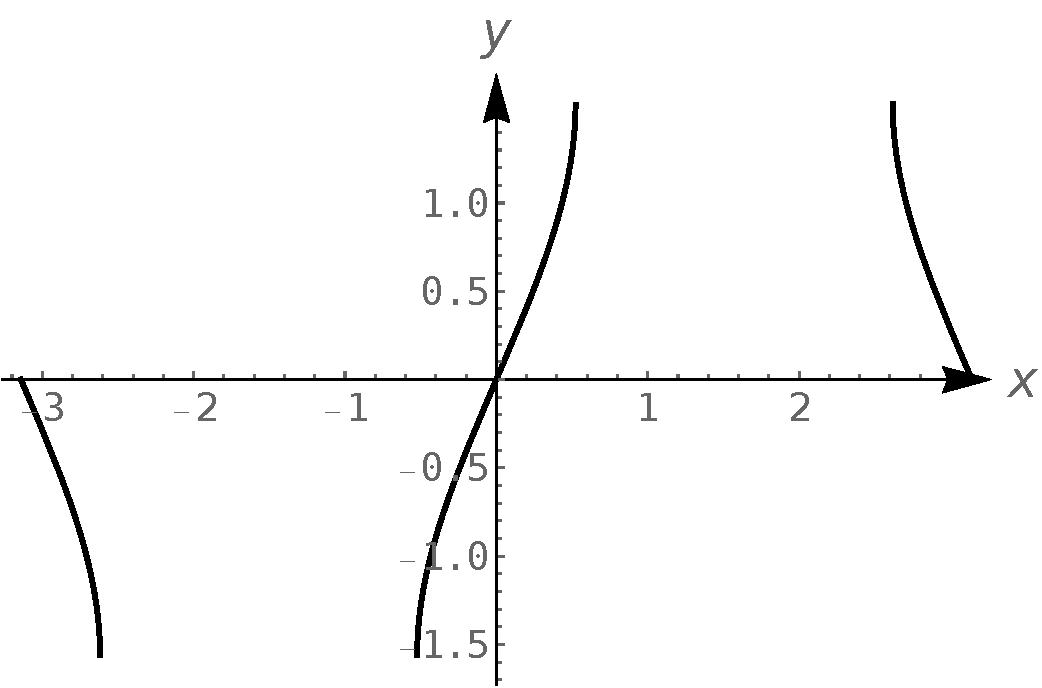
\includegraphics[width=0.32\textwidth]{grafs_3}}
%(-x,-y)
%\hspace*{0.5cm}
%\subfigure[]{\includegraphics[width=0.33\textwidth]{grafs_6}}
\hspace*{0.5cm}
\subfigure[]{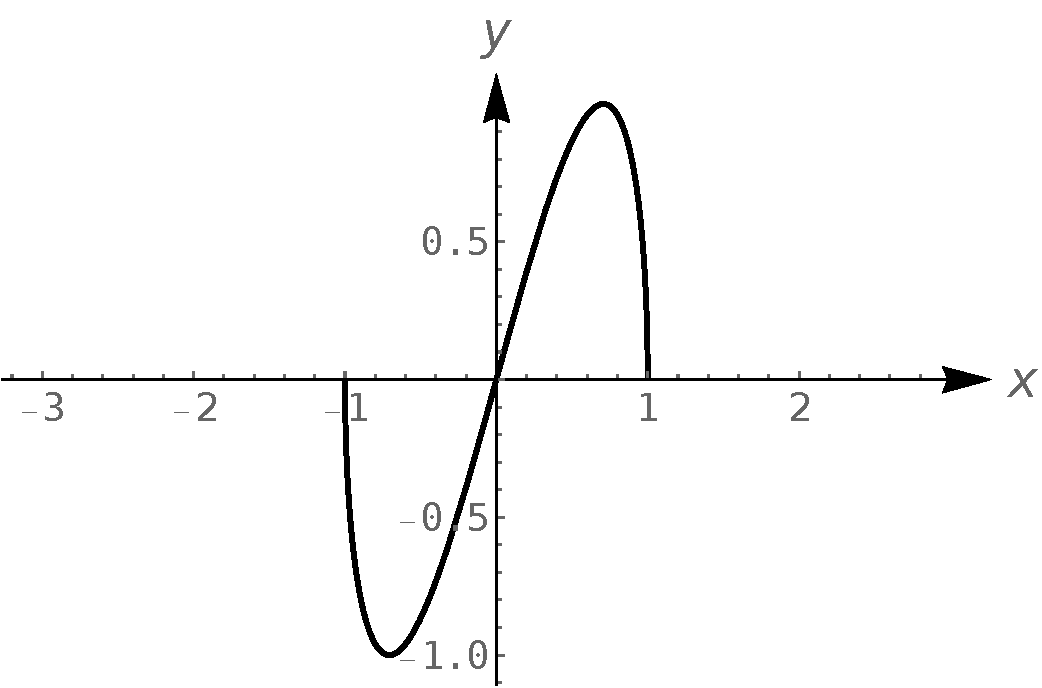
\includegraphics[width=0.32\textwidth]{grafs_1}}
%(0,x)
}
\centerline{
%\subfigure[]{\includegraphics[width=0.33\textwidth]{grafs_5}}
%\hspace*{0.5cm}
\subfigure[]{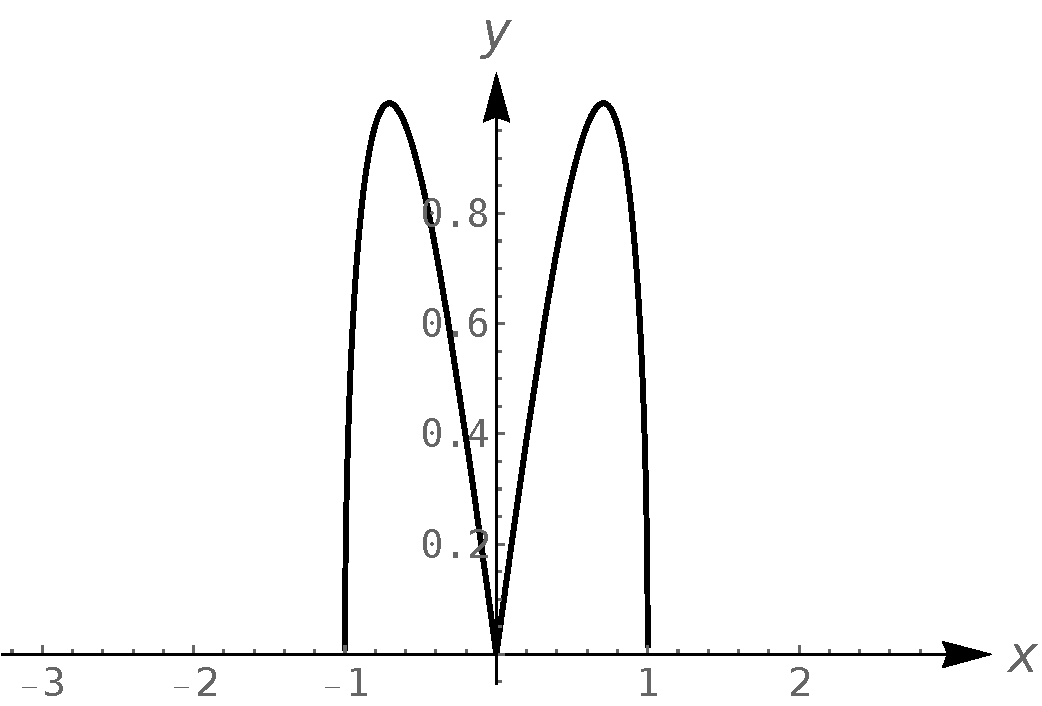
\includegraphics[width=0.32\textwidth]{grafs_2}}
%(-x,-y)
\hspace*{0.5cm}
\subfigure[]{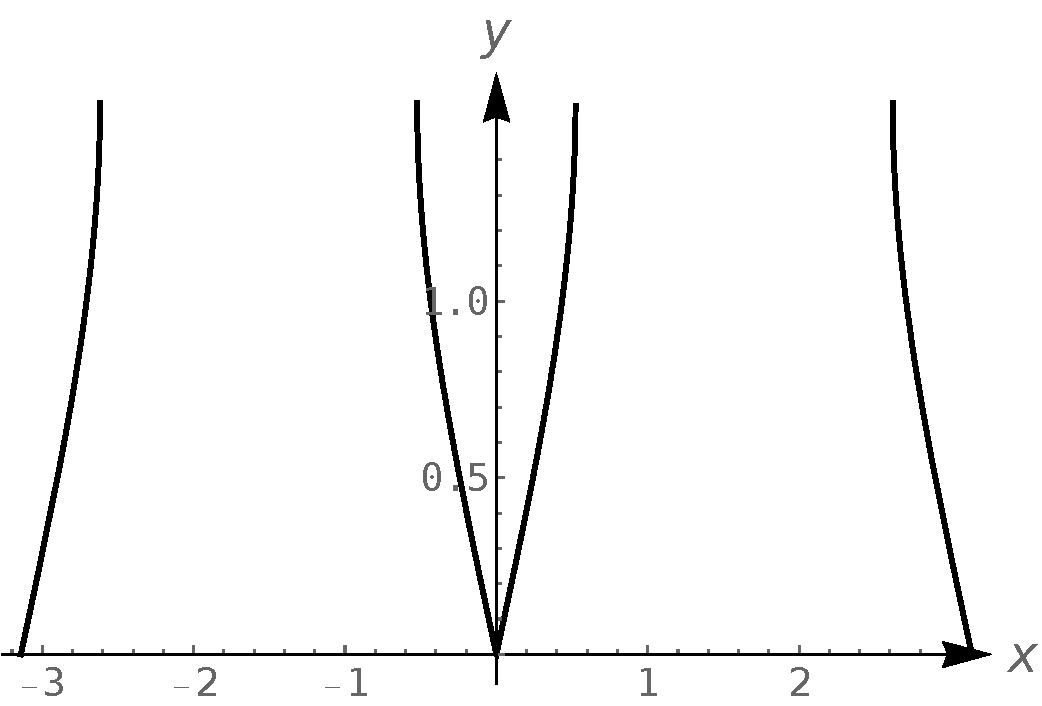
\includegraphics[width=0.32\textwidth]{grafs_4}}
%(0,x)
}
\caption{\label{grafs}}
\end{figure}
\end{Exercise}

\begin{Answer}
\begin{multicols}{2}

\Question $y=\sin(2\arcsin(x))$ - graph b
\Question  $y=\sin(2\arcsin(|x|))$ - graph c
\Question  $y=\sin(2|\arcsin(x)|)$ - graph c
\Question  $y=\arcsin(2\sin(x))$ - graph a
\Question  $y=\arcsin(2\sin(|x|))$ - graph d
\Question  $y=\arcsin(2|\sin(x)|)$ - graph d
 \EndCurrentQuestion
\end{multicols}
\end{Answer}

\begin{Exercise} %{\bf (0.5p, *)} 
Determine the value(s) of the parameter $p$ for which the following function is increasing on $]-\infty,+\infty[$
$$
f(x)=p\,x+\dfrac{1}{x^2+3}\,.
$$
\end{Exercise}

\begin{Answer}\phantom{}
$p \geq \dfrac{1}{8}$
\end{Answer}

\begin{Exercise} %{\bf (3p)} 
For each of the problems below, construct the integral that allows you to calculate what is asked:
\Question the area of the region bounded by $y=x^3$, $y=0$ and the tangent line in $(-1,-1)$ to the graph of $y=x^3$.
\Question the volume of the body created by rotating the region enclosed between $y=-x^2+1$ and $y=x^2-3$ about the line $y=-4$.
\Question the distance traveled by a particle moving between $t=0$ and $t=1$ along the curve $C$ parameterised by $\vec{r}(t)=\left(2t^{3/2},\cos(2t),\sin(2t)\right)$;
\Question the work done by a particle moving from $(1,1,1)$ to $(2,4,8)$ along the curve $C$ parametrised by $\vec{r}(t)=\left(t,t^2,t^3\right)$ and subject to the field $\vec{F}=\left(\sin(x),\sin(y),\sin(z)\right)$.
\EndCurrentQuestion
\end{Exercise}

\begin{Answer}\phantom{}

\Question There are two possible areas. Giving one of them is enough. \\

$A = \displaystyle \int \limits_{-1}^0 \int\limits_{\frac{y-2}{3}}^{\sqrt[3]{y}} \, dx dy $ \quad or \quad $A= \displaystyle  \int\limits_{-2/3}^0 \int\limits_{0}^{3x+2} \, dy dx + \int\limits_{0}^2 \int\limits_{x^3}^{3x+2} \, dy dx$ 
\Question $V = 2x \displaystyle \int\limits_{0}^{\sqrt{2}} \pi \left( - x^{*2}+5 \right)^2 dx^* - 2x \displaystyle \int\limits_{0}^{\sqrt{2}} \pi \left( x^{*2}+1 \right)^2 dx^*$ \quad where $y^* = y+4$ \; and \; $x^* = x$
\Question $L= \displaystyle \int\limits_{0}^{1} \sqrt{9t + 4 \sin^2(2t) + 4 \cos^2(2t)} \, dt= \displaystyle \int\limits_{0}^{1} \sqrt{9t + 4 } \, dt$
\Question $W = \displaystyle \int\limits_{1}^{2} \left(\sin(t), \sin\left(t^2 \right), \sin\left(t^3 \right) \right) \cdot \left( 1, 2t, 3t^2\right) \, dt $
\end{Answer}

\begin{Exercise} %{\bf (1p, **)} 
Calculate
$$
I = \int\limits_0^1\int\limits_{\arcsin(y)}^{\frac{\pi}{2}}\cos(x)\sqrt{1+\cos^2(x)}\,dx\,dy\,.
$$
\end{Exercise} 

\begin{Answer}\phantom{}
$I = -\dfrac{1}{3} + \dfrac{2^{3/2}}{3}$
\end{Answer}



\begin{Exercise} % {\bf (0.5p, *)} 
Change the order of integration in
$$
I = \int\limits_{-1}^1\int\limits_{x^2}^1\int\limits_0^{1-y}f(x,y,z)\, dz\,dy\,dx
$$
to $dx\,dy\,dz$.
\end{Exercise}

\begin{Answer}\phantom{}
$I = 2 \displaystyle\int\limits_{0}^1\int\limits_{0}^{1-z}\int\limits_0^{\sqrt{y}}f(x,y,z)\, dx\,dy\,dz$
\end{Answer}


\begin{Exercise} %  {\bf (1p, **)} 
Determine the value(s) of the parameter $p$ for which the following series converges
$$
\sum\limits_{n=3}^{+\infty}\dfrac{1}{n\ln(n)\Big[\ln\big(\ln(n)\big)\Big]^p}\,.
$$
\end{Exercise}

\begin{Answer}\phantom{}
The series converges for $p > 1$. 
\end{Answer}


\begin{Exercise} % {\bf (0.5p, *)} 
Show that for $n\in\mathbb{Z}$ it holds that
$$
\int\limits_{0}^{1}\dfrac{\cos(nx)}{x+1} \, dx\leq\ln(2)\,.
$$
\end{Exercise}

\begin{Answer}\phantom{}
$\displaystyle \int\limits_{0}^{1}\dfrac{\cos(nx)}{x+1} \, dx \leq \int\limits_{0}^{1}\dfrac{1}{x+1} \, dx   \leq\ln(2)$. We can make this estimate, independent of the argument of the cosine, because the image of the cosine is limited to $[-1,1]$.
\end{Answer}

\begin{Exercise} %  {\bf (1p, ***)} 
Determine the MacLaurin series expansion of the second order of
$$
f(x)=\int\limits_{-x}^{3\cos(x)}\cos\left(xt^2\right)dt\,.
$$
\end{Exercise}

\begin{Answer}\phantom{}
$f(x) = 3 + x - \dfrac{1}{2} \dfrac{258}{5}x^2 + \ldots $
\end{Answer}


\begin{Exercise} %  {\bf (1p, *)} 
Show that $f(x,y)= x^2+4y^2-4xy+2$ has an infinite number of critical points and that these are all minima.
\end{Exercise}

\begin{Answer}\phantom{}
The critical points are solutions of $\partial f/ \partial x = 0$ and $\partial f/ \partial y = 0$. We find infinitely many critical points along the line $y= x/2$. If we write $f(x,y)$ as $f(x,y) = (x-2y)^2 + 2$, then it immediately follows that the function values in points not located on the line are higher than those that are reached for points on the line. 
\end{Answer}


\begin{Exercise} %   {\bf (2p, ***)} 
The cat Kamu is sleeping peacefully after a strenuous day. However, a mouse has planned an attack on Kamu and is moving with a helicoidal trajectory
given by
$$
\vec{r}(t)=6\cos(\pi\,t)\hat{i}+6\sin(\pi\,t)\hat{j}+2t\hat{k}\,,
$$
where $t\geq0$, in the direction of Kamu, who can be represented as a sphere with cartesian equation
$$
x^2+y^2+z^2=100\,.
$$
\Question Determine when the mouse arrives at Kamu's skin surface.
\Question Determine where the mouse bites Kamu.
\Question Determine at which angle this happens, i.e.\ which angle does the skin surface make with the mouse when it inflicts the bite.
\EndCurrentQuestion
\end{Exercise}

\begin{Answer}\phantom{}
\begin{multicols}{2}
\Question $t=4$
\Question $\vec{r}(4) = (6,0,8)$
\Question $\dfrac{\pi}{2} - \arccos\left(\dfrac{-8}{5 \sqrt{36 \pi^2 + 4}} \right)$
 \EndCurrentQuestion
\end{multicols}

\end{Answer}


%%%%%%%%%%%%%%%%%%%%%%%%%%%
%Examen aug 2019 (Wiskunde 2)
%%%%%%%%%%%%%%%%%%%%%%%%%%%
\section{Exam August 2019}
%\begin{enumerate}

\begin{Exercise} %{\bf (1.5 p, *)} 
For each statement, indicate whether it is true or false. Also briefly motivate your answer.

\Question Let $A$ and $B$ be non-empty, bounded subsets of $\mathbb{R}$. If sup $A$ = inf $B$, then for every element $a$ of $A$ there exists an element $b$ of $B$ such that $a \leq b$.
	%JUIST
	
\Question The graph of $r\left(\theta\right)=4\cos(\theta-\pi/3)$, $0\leq\theta\leq\pi$, is not a circle.
	% Fout: varberg p552
	
\Question Each contour surface of a function of three variables can be seen as a surface in three-dimensional space. 
	% Uit:multivar_meerkeuze p19
	% Fout: punt bijv
	
\Question Figure \ref{fig_zadeloppervlak} shows the surface $z=f(x,y)$. We can conclude that $f_{xx}(P) >0$ and $f_{yy}(P) <0$. \label{vraag_zadeloppervlak}
	 \begin{figure}[H]
		\centering
		%\raisebox{0.5cm}{
		\centerline{
			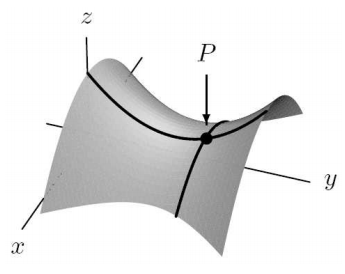
\includegraphics[width=0.3\textwidth]{zadelopp}
		}
		\caption{Surface $z=f(x,y)$ from Question~\ref{vraag_zadeloppervlak}.}
		\label{fig_zadeloppervlak}
	\end{figure}
	
\Question Consider a point $P$ on a curve $C$ for which there are two different parameterisations, \ $\vec{r}_1(t)$ and $\vec{r}_2(t)$. Then the tangent vector of $\vec{r}_1(t)$ in $P$ is the same as the one of $\vec{r}_2(t)$.
	% Uit:multivar_meerkeuze2 p6
	% Fout: zie voorbeeld 18.2 en aanvulling les
	
\Question Consider the vector field $\vec{F}(x,y,z) = (x+\sin(y), y - \sin(z), z)$. The divergence of this vector field is $(1,1,1)$.
	%FOUT: div F = 3
\EndCurrentQuestion
\end{Exercise}

\begin{Answer}

\Question True. Let $a$ be any element of $A$. Since sup $A$ is an upper bound for $A$, $a \leq$ sup $A = $ inf $B$. Since inf $B$ is a lower bound for $B$, $a$ will be smaller than or equal to any element of $B$. So there exists a $b \in B$ such that $a \leq b$.
\Question False. The graph is in fact a circle with center along $\theta = \pi/3$ and radius 2.
\Question False. A contour surface can be a surface, but also, for example, a point. 
\Question False. $f_{xx}(P) <0$ and $f_{yy}(P) > 0$.
\Question False. As an example, take the circle $x^2 + y^2 = 4$ and parameterise it in two different ways. Also calculate the tangent vector.
\Question False. The divergence is a number and not a vector. Verify that it is equal to 3.
\end{Answer}



\begin{Exercise} %{\bf (0.75p, **)} 
Determine the corresponding function rule for each graph in Figure~\ref{grafs_par_eq}.
\Question $x(t)=t^4-t+1, \quad y(t)=t^2$
\Question $x(t)=t^2-2t,  \quad y(t)=\sqrt{t}$
\Question $x(t)=\sin(2t),  \quad y(t)=\sin(t+\sin(2t))$
\Question $x(t)=\cos(5t),  \quad y(t)=\sin(2t)$
\EndCurrentQuestion
\begin{figure}[H]
\centering
\centerline{
\subfigure[]{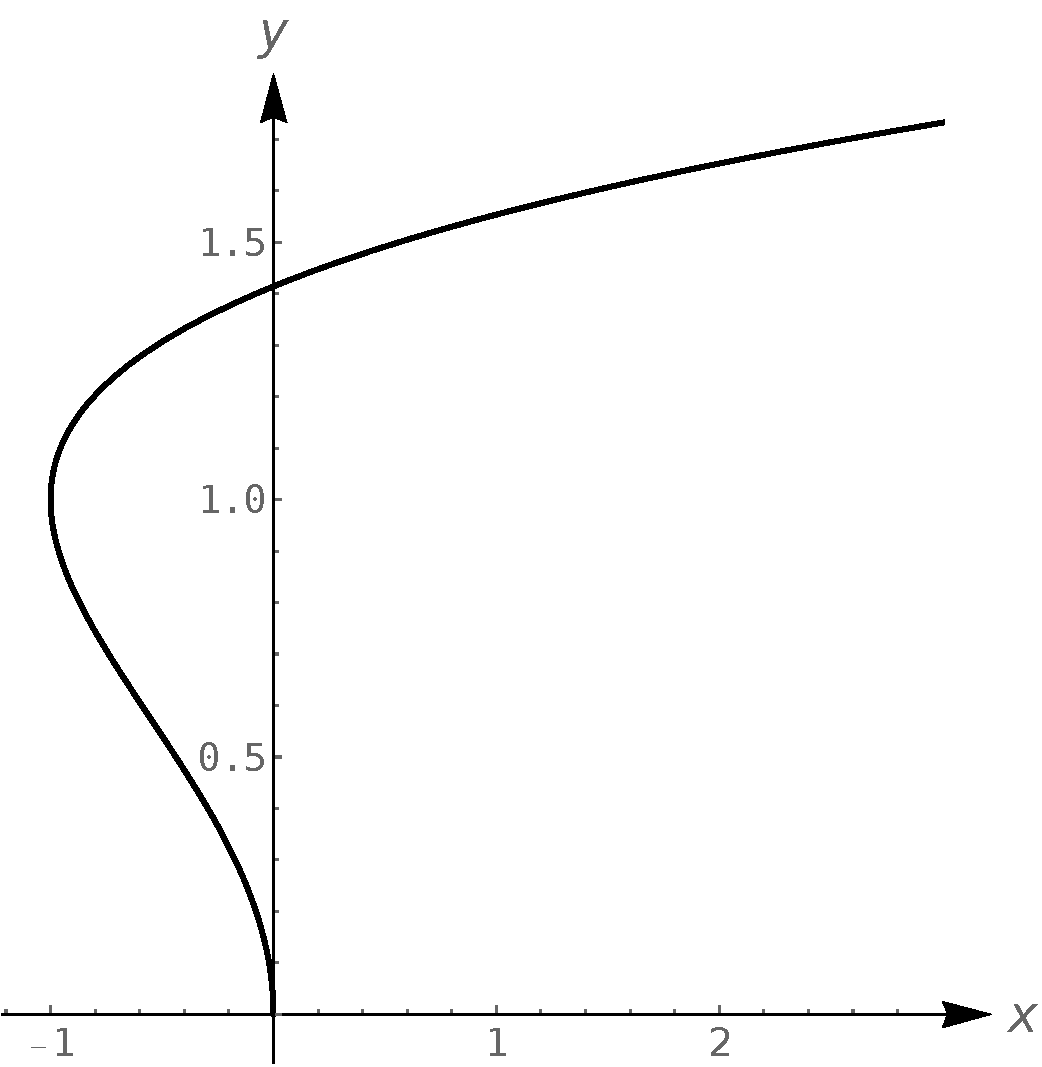
\includegraphics[width=0.32\textwidth]{parametric_eq_2-a}}
\hspace*{0.5cm}
\subfigure[]{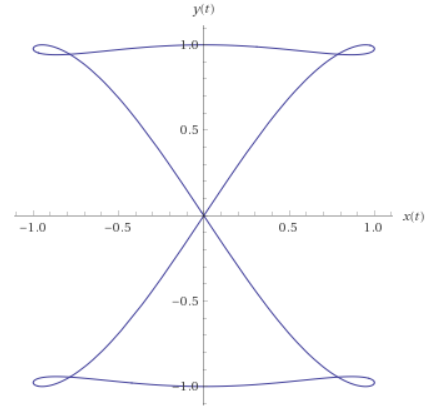
\includegraphics[width=0.32\textwidth]{parametric_eq_3-b}}
}
\centerline{
\subfigure[]{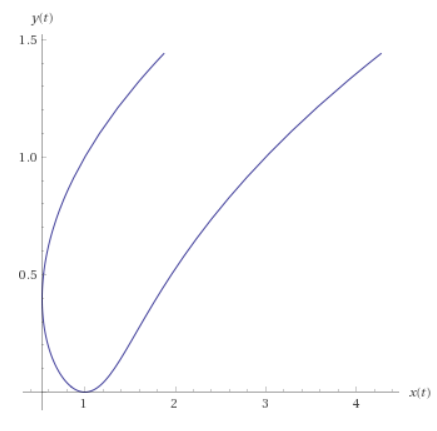
\includegraphics[width=0.32\textwidth]{parametric_eq_1-e}}
\hspace*{0.5cm}
\subfigure[]{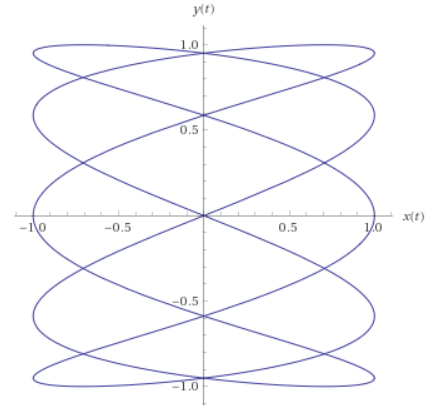
\includegraphics[width=0.32\textwidth]{parametric_eq_4-f}}
}
\caption{\label{grafs_par_eq}}
\end{figure}
\end{Exercise}

\begin{Answer}

\Question  $x(t)=t^4-t+1, \quad y(t)=t^2$ \; - graph c 
\Question  $x(t)=t^2-2t,\quad y(t)=\sqrt{t}$ \; - graph a
\Question $x(t)=\sin(2t), \quad y(t)=\sin(t+\sin(2t))$ \; - graph b
\Question  $x(t)=\cos(5t),  \quad y(t)=\sin(2t)$ \; - graph d

\end{Answer}



\begin{Exercise} %{\bf (1p, *)} 
Find out where the $f$ function below is continuous and differentiable. %Bio-irs

\[ f(x)= \left\{\begin{array}{rcl} 
\tan(x), & \text{ if} & x<0, \\
x, & \text{ if} & 0 \leq x <1, \\
1 + \ln(x), & \text{ if} & 1 \leq x. 
\end{array}  \right.   \]
\end{Exercise} 

\begin{Answer}

\Question $x<0$: the function is continuous and differentiable on the domain of the tangent.
\Question $0 \leq x < 1$: the function is continuous and differentiable.
\Question $x \geq 1$: the function is continuous and differentiable.

\end{Answer}

\begin{Exercise} %{\bf (1.5p, **)} 
Discuss 
$$
\lim\limits_{x\to0}x^p\left(1-\sqrt{1+x}\right)
$$
as a function of the parameter $p\in\mathbb{Z}$. %Bio-irs
\end{Exercise}

\begin{Answer}

\Question $p \geq 0: \lim\limits_{x\to0}x^p\left(1-\sqrt{1+x}\right) = 0$
\Question $p < 0:$
\begin{itemize}
    \item $p <-1: \lim\limits_{x \to 0}x^p\left(1-\sqrt{1+x}\right) = \pm \infty$
    \item $p =-1: \lim\limits_{x \to 0}x^p\left(1-\sqrt{1+x}\right) = -\dfrac{1}{2}$
    \item $p >-1: \lim\limits_{x \to 0}x^p\left(1-\sqrt{1+x}\right) = 0$
\end{itemize}

\end{Answer}


\begin{Exercise} %{\bf (1p, *)} 
A water reservoir has a parabolic shape and is formed by the rotation of the parabola $y=ax^2$ about the $y$-axis. The maximum water depth in this reservoir is 8 m and when the reservoir is filled to a height of 5 m, the water surface has a diameter of 20 m. What is the maximum volume of water that this reservoir can hold?
\end{Exercise}

\begin{Answer}\phantom{}
$V = 8 \pi \left(\sqrt{160} \right)^2 - 2 \pi \displaystyle \int\limits_0^{\sqrt{160}} \dfrac{x^3}{20} \, dx$
\end{Answer}

\begin{Exercise} %{\bf (1,5p, **)}
Consider the following theorem.
\begin{theorem}[Generalised mean value theorem]
	Let $f$ and $g$ be two continuous functions on $[a,b]$ and differentiable on $]a,b[$. If $g'(x) \neq 0$ for every $x \in\, ]a,b[$, then there exists a $c \in \, ]a,b[$ such that 
	\[ \dfrac{f(b)-f(a)}{g(b)-g(a)} = \dfrac{f'(c)}{g'(c)}. \]
\end{theorem} 

Below is an attempt to prove this theorem, but it contains a couple of logical errors. Correct these errors. \npar

%%%%%%%%%%%%%%%
%Foute versie
%%%%%%%%%%%%%%%
From $g'(x) \neq 0$, for every $x \in\, ]a,b[$, it follows that $g(b) \neq g(a)$. Otherwise, $g'$ would equal 0 for every $c \in \, ]a,b[$. \\
We apply the mean value theorem to the function
\[h(x) = \left( f(b)-f(a) \right) \left(g(x)-g(a) \right) - \left( g(b)-g(a) \right) \left(f(x)-f(a) \right).  \]
Since $h(a)=h(b) \neq0$, for every $c\in\, ]a,b[$, it will hold that $h'(c)=0$. We obtain
\[ f'(c)\left( g(x)-g(a) \right)  - g'(c) \left( f(x)-f(a) \right) =0,\]
From which it follows that
\[ \dfrac{f(b)-f(a)}{g(b)-g(a)} = \dfrac{f'(c)}{g'(c)}. \]

\end{Exercise}

\begin{Answer}\phantom{}
Correct proof of the theorem below.
\begin{theorem}[Generalised mean value theorem]
    Let $f$ and $g$ be two continuous functions on $[a,b]$ and differentiable on $]a,b[$. If $g'(x) \neq 0$ for every $x \in\, ]a,b[$, then there exists a $c \in \, ]a,b[$ such that 
	\[ \dfrac{f(b)-f(a)}{g(b)-g(a)} = \dfrac{f'(c)}{g'(c)}. \]
\end{theorem} 
    
From $g'(x) \neq 0$, for every $x \in\, ]a,b[$, it follows that $g(b) \neq g(a)$. Otherwise, there would exist a number in $]a,b[$ for which $g'$ equals 0. \\
We apply Rolle's theorem to the function
\[h(x) = \left( f(b)-f(a) \right) \left(g(x)-g(a) \right) - \left( g(b)-g(a) \right) \left(f(x)-f(a) \right).  \]
Since $h(a)=h(b)=0$, there exists a $c\in\, ]a,b[$ such that $h'(c)=0$. We obtain 
\[ \left( f(b)-f(a) \right) g'(c) - \left( g(b)-g(a) \right) f'(c)=0,\]
from which it follows that
\[ \dfrac{f(b)-f(a)}{g(b)-g(a)} = \dfrac{f'(c)}{g'(c)}. \]
\end{Answer}


\begin{Exercise} %{\bf (3.5p)} 
For each of the problems below, construct the integral that allows you to calculate what is asked. Write the integrandum as simply as possible.
\Question %[(a, **)] 
the area of the region outside $r=a$ and bounded by $r=2a\cos(3\theta)$. %Bio-irs
\Question %[(b, *)] 
the surface area of $2z=x^2+y^2$, cut off by $x^2+y^2=1$. %Bio-irs
%\item [(d, ?)] de manteloppervlakte van $x^2+y^2+z^2=4$, afgesneden door $x^2+y^2=2y$. %Bio-irs
\Question %[(c, **)] 
the line integral of $\vec{V}=\left(x^2+y,xy+2y^2\right)$ along the closed curve $K$ where $K$ connects the points $A(0,0)$, $B(5.0)$ and $C(0 \sqrt{20})$. $AB$ and $CA$ are line segments and $BC$ is the part of the ellipse $4x^2+5y^2=100$ in the first quadrant. %Bio-irs
\EndCurrentQuestion
\end{Exercise}

\begin{Answer}

\Question $A = 6 . \dfrac{1}{2} \displaystyle \int \limits_0^{\pi/9} \left( \left( 2a \cos(3\theta) \right)^2 - a^2 \right) \, d \theta $ 

\Question $SA = \displaystyle \int \limits_0^{2\pi} \int \limits_0^{1} \sqrt{1+r^2} r\, dr d \theta $ 

\Question $\displaystyle \oint_K  \vec{V} \cdot d\vec{r} = \displaystyle \int \limits_0^{5} \int \limits_0^{\sqrt{\frac{100 - 4x^2}{5}}} (y-1)\, dy d x $ \quad (Green's theorem)
   

\end{Answer}



\begin{Exercise}  %{\bf (1p, *)} 
Determine the convergence of
$$
\sum\limits_{n=1}^{+\infty}\dfrac{(-1)^n}{\cosh(n)}\,.
$$
%Bio-irs
\end{Exercise}

\begin{Answer}\phantom{}
The alternating series is absolutely convergent.
\end{Answer}

\begin{Exercise} %{\bf (2.5p, ***)} 
We consider the function $f(x)$ which we can approximate with a Taylor series of the $n$-th order in the point $a$. We write $f$ as
\[f(x) = T_n(x) + R_n(x),  \]
where $T_n(x)$ is the Taylor polynomial of the $n$-th order of $f$ in $a$ and $R_n(x)$ is the remainder of this sequence which can be written as follows.\\
\begin{theorem}[Alternative formulation for the remainder]
Let $f^{(n+1)}$ be continuous on an open interval $I$ containing $a$ and $x$, then
\[R_n(x) = \dfrac{1}{n!} \int\limits_{a}^{x} (x-t)^n f^{(n+1)} (t) \, dt. \]
\end{theorem}

We prove this theorem below by means of mathematical induction. Complete in this bundle where you find a dotted line. \\

For $n=1$ it holds that
\\[0.5cm]
\[R_1(x) = f(x) - T_1(x) = \dotrule{0.70\textwidth}%f(x)-f(a)-f'(a)(x-a), 
\]
\\[0.5cm]
and the integral in the theorem becomes
\\[0.5cm]
\[\dotrule{0.95\textwidth}%\int\limits_{a}^{x} (x-t) f'' (t) \, dt
\]
\\[0.5cm]
We calculate this integral by using integration by parts with
\\[0.2cm]
\[ u(t) = \dotrule{0.30\textwidth} \quad \text{ and } \quad dv(t) = \dotrule{0.30\textwidth},\]
\\[0.2cm]
from which it follows that
\[ du(t) = -dt \quad \text{ and } \quad v(t) = \dotrule{0.30\textwidth}.\]
Thus, the integral becomes
\begin{align*}
&\int\limits_{a}^{x} \dotrule{0.50\textwidth} \, dt	\\[0.75cm]
&= \dotrule{0.80\textwidth} \\[0.75cm]
&= \dotrule{0.80\textwidth} \\[0.75cm]
&=\dotrule{0.80\textwidth} \\[0.75cm]
&= R_1(x).	
\end{align*}
This proves the theorem for $n=1$. \npar

We assume that the theorem holds for $n=k$, so
\\[0.5cm]
\[R_k(x) = \dotrule{0.80\textwidth} %\dfrac{1}{k!} \int\limits_{a}^{x} (x-t)^k f^{(k+1)} (t) \, dt. 
\]
\\[0.5cm]
We then prove the theorem for $n=k+1$, so
\\[0.5cm]
\[R_{k+1}(x) = \dotrule{0.80\textwidth} %\dfrac{1}{(k+1)!} \int\limits_{a}^{x} (x-t)^{k+1} f^{(k+2)} (t) \, dt. 
\]
\\[0.5cm]
We again use integration by parts to calculate this last integral. We set
\\[0.2cm]
\[ u(t) = \dotrule{0.30\textwidth} \quad \text{ and } \quad dv(t) = \dotrule{0.30\textwidth},\]
\\[0.2cm]
from which it follows that
\[ du(t) = -(k+1)(x-t)^k \,dt \quad \text{ and } \quad v(t) = \dotrule{0.30\textwidth}.\]
The integral is thus
\begin{align*}
	& \dfrac{1}{(k+1)!} \int\limits_{a}^{x} \dotrule{0.50\textwidth} \, dt \\[0.75cm]	
	&= \dotrule{0.80\textwidth} \\[0.75cm]
	&= \dotrule{0.80\textwidth} \\[0.75cm]
	&= - \dfrac{f^{(k+1)}(a)}{(k+1)!}(x-a)^{k+1} + R_k(x) \\[0.75cm]
	&= f(x) - \dotrule{0.72\textwidth} \\[0.75cm]
	&= f(x) - \dotrule{0.72\textwidth} \\[0.75cm]
	&= R_{k+1}(x). \\	
\end{align*}

The theorem is valid for $n=k+1$ if it is valid for $n=k$, therefore it is valid for all $n \in \mathbb{N}$.
\end{Exercise}

\begin{Answer}
    We consider the function $f(x)$ which we can approximate with a Taylor series of the $n$-th order in the point $a$. We write $f$ as
    \[f(x) = T_n(x) + R_n(x),  \]
    where $T_n(x)$ is the Taylor polynomial of the $n$-th order of $f$ in $a$ and $R_n(x)$ is the remainder term of this sequence which can be written as follows.\\
    \begin{theorem}[The remainder term of a Taylor series]
    Let $f^{(n+1)}$ be continuous on an open interval $I$ containing $a$ and $x$, then
    \[R_n(x) = \dfrac{1}{n!} \int\limits_{a}^{x} (x-t)^n f^{(n+1)} (t) \, dt. \]
    \end{theorem}
    
    We prove this theorem below by means of mathematical induction. 
    
    
    For $n=1$ it holds that
    \[R_1(x) = f(x) - T_1(x) = f(x)-f(a)-f'(a)(x-a),\]
    and the integral in the theorem becomes
    \[\int\limits_{a}^{x} (x-t)\  f'' (t) \, dt.
    \]
    We calculate this integral by using integration by parts with
    \[ u(t) = x-t \quad \text{ en } \quad dv(t) = f''(t)\, dt,\]
    from which it follows that
    \[ du(t) = -dt \quad \text{ en } \quad v(t) = f'(t).\]
    Thus, the integral becomes
    \begin{eqnarray*}
    \int\limits_{a}^{x} (x-t) \ f''(t) \, dt
    &=& \left[ (x-t) \ f'(t) \right]_a^x + \ds \int \limits_a^x f'(t) \ dt \\
    &=& 0-(x-a)\ f'(a) + f(x) - f(a) \\
    &=&f(x)-f(a)-f'(a)(x-a) = R_1(x).	
    \end{eqnarray*}
    This proves the theorem for $n=1$. \npar
    
    We assume that the theorem holds for $n=k$, so
    \[R_k(x) = \dfrac{1}{k!} \int\limits_{a}^{x} (x-t)^k f^{(k+1)} (t) \, dt. 
    \]
    We then prove the theorem for $n=k+1$, so
    \[R_{k+1}(x) = \dfrac{1}{(k+1)!} \int\limits_{a}^{x} (x-t)^{k+1} f^{(k+2)} (t) \, dt. 
    \]
    We again use integration by parts to calculate this last integral. We set
    \[ u(t) = (x-t)^{k+1} \quad \text{ and } \quad dv(t) = f^{(k+2)}(t) \, dt,\]
    from which it follows that
    \[ du(t) = -(k+1)(x-t)^k \,dt \quad \text{ and } \quad v(t) = f^{(k+1)}(t).\]
    The integral is thus
    \begin{eqnarray*}
    \dfrac{1}{(k+1)!} \int\limits_{a}^{x} (x-t)^{k+1}\ f^{(k+2)}(t) \, dt 
        &=& \dfrac{1}{(k+1)!} \left[(x-t)^{k+1}\ f^{(k+1)}(t)\right]_a^x + \dfrac{k+1}{(k+1)!}\int\limits_{a}^{x} (x-t)^{k}\ f^{(k+1)}(t) \, dt \\
    	&=& 0 - \dfrac{1}{(k+1)!} (x-a)^{k+1}\ f^{(k+1)}(a)  + \dfrac{1}{k!}\int\limits_{a}^{x} (x-t)^{k}\ f^{(k+1)}(t) \, dt \\
    	&=& - \dfrac{f^{(k+1)}(a)}{(k+1)!}(x-a)^{k+1} + R_k(x) \\ 
    	&=& f(x) - T_k(x) - \dfrac{f^{(k+1)}(a)}{(k+1)!}(x-a)^{k+1} \\ 
    	&=& f(x) - T_{k+1}(x) = R_{k+1}(x). 	
    \end{eqnarray*}
    
    The theorem is valid for $n=k+1$ if it is valid for $n=k$, therefore it is valid for all $n \in \mathbb{N}$.
\end{Answer}



\begin{Exercise} %{\bf (2p, **)} 
Consider the surface
\[z + \ln(z)-xy=0 \,.
\]
\Question Show that the above relation determines $z$ as an implicit function of $x$ and $y$ in an environment of $(1/2,2,1)$.
\Question Determine the equation of the tangent plane to the surface at the point \\ $(1/2,2,1)$.
\Question Determine 
\[\dfrac{\partial^2 z}{\partial x \partial y}. \]
%Bio-irs
\EndCurrentQuestion
\end{Exercise}

\begin{Answer}

\Question Verify that the point is on the surface. Then verify the condition $\partial F / \partial z \neq 0$ in the given point. 
\Question $ \left(x - \dfrac{1}{2} \right) + \dfrac{1}{4}\left(y-2 \right) - \left(z-1 \right) =0  $
\Question $\dfrac{\partial^2 z}{\partial x \partial y} = \dfrac{z(z+1)^2 + xyz }{(z+1)^3}$

\end{Answer}


\begin{Exercise} %{\bf (1.5p, *)} 
Consider the double integral
\[
I = \int\limits_0^2\int\limits_{0}^{\sqrt{4-y^2}}(x^2+y^2)\,dx\,dy\,.
\]
\Question Rewrite $I$ in polar coordinates. 
\Question Rewrite $I$ as a triple integral in cylinder coordinates.
%Bio-irs
\EndCurrentQuestion
\end{Exercise}

\begin{Answer}

\Question $I = \displaystyle \int \limits_0^{\pi/2} \int \limits_0^{2} r^2 \ r\, dr d \theta $ 
\Question $I = \displaystyle \int \limits_0^{\pi/2} \int \limits_0^{2} \int \limits_0^{r^2} r\,dz dr d \theta $ 

\end{Answer}



\begin{Exercise} %{\bf (1.25p, **)} 
Consider the double integral
\[I=\iint\limits_{D}f(x,y)\,dy\,dx \]
with $D$ the area within $(x-1)^2 + (y-1)^2 = 2$ \'and on the convex side of \\ $(y-1)^2=1-2x$. Give $x$ and $y$ concrete boundaries.
%Bio-irs
\end{Exercise}

\begin{Answer}

\Question[]You can consider three regions.
\Question Region 1: $x: 0 \rightarrow \dfrac{1}{2}, \quad y: 1 - \sqrt{2-(x-1)^2} \rightarrow 1 - \sqrt{1-2x}$
\Question Region 2: $x: 0 \rightarrow \dfrac{1}{2}, \quad y: 1 + \sqrt{1-2x} \rightarrow 1 + \sqrt{2-(x-1)^2}$
\Question Region 3: $x: \dfrac{1}{2} \rightarrow 1+\sqrt{2}, \quad y: 1 - \sqrt{2-(x-1)^2} \rightarrow 1 + \sqrt{2-(x-1)^2}$

\end{Answer}



\begin{Exercise} %{\bf (1p, **)} 
Calculate
$$
I = \int\limits_{-\infty}^{+\infty}\int\limits_{-\infty}^{+\infty}\int\limits_{-\infty}^{+\infty}\sqrt{x^2+y^2+z^2}e^{-\left(x^2+y^2+z^2\right)} dx\,dy\,dz.
$$
%Antw: 2\pi
\end{Exercise}
%\end{enumerate}
\begin{Answer}
$I = 2 \pi$

\end{Answer}



%%%%%%%%%%%%%%%%%%%%%%%%%%%
%Examen januari 2020
%%%%%%%%%%%%%%%%%%%%%%%%%%%
\section{Exam January 2020}

\begin{Exercise} %{\bf (1p)} 
For each statement, indicate whether it is true or false. Also briefly motivate your answer.

\Question If
    $$
    f(x)=\dfrac{x^2-1}{x+1}\qquad\text{and}\qquad g(x)=x-1\,,
    $$
    then it holds that $f(x)=g(x)$.
	% FALSE
	
\Question If $x=1$ is a vertical asymptote of the graph of $y=f(x)$, then the function $f(x)$ is not defined at $x=1$.

\Question The curves $4=r\cos(\theta-2\pi/5)$ and $\theta = 2 \pi/5 $ determine (half-)lines that are perpendicular to each other.
	%True

\Question If $f(x)$ has a Taylor series expansion around $x_0=0$ with radius of convergence $R$, than
    $$
    g(x) = f\left(\frac{x-1}{2}\right)
    $$
    has a Taylor series expansion around $x_0=1$ with radius of convergence $2R$.
    % Juist
\EndCurrentQuestion
\end{Exercise}

\begin{Answer}

\Question False. The functions are equal for $x \neq -1$. At $x=-1$ a perforation occurs.
\Question True. $f(x)$ is not defined at $x=1$, because $\displaystyle \lim_{x \to 1} f(x) = \pm \infty$. \\
OR: False. There may be a removable discontinuity. Find a counterexample yourself.
\Question True. Determine the Cartesian equation and/or direction and conclude that the product of the slopes equals $-1$. This means that the (half-)lines are perpendicular to each other. 
\Question True. Convert the convergence interval for $x$ to one for $(x-1)/2$.

\end{Answer}



\begin{Exercise} %{\bf (2p)} 
Use the $(\epsilon,\delta)$ definition to show that
$$
\lim_{x\underset{>}{\rightarrow}4}\sqrt{x-4}=0\,.
$$
\end{Exercise}

\begin{Answer}\phantom{}
Do this yourself. In the proof, choose $\delta = \epsilon^2$.
\end{Answer}


\begin{Exercise} % {\bf (3p)} 
Consider the real-valued function $f$:
$$
f(x)=\dfrac{\ln\left(\ln\left(x^2\right)\right)}{2x^3-4x}\,.
$$
\Question Determine the domain of $f$.
\Question Determine whether $f$ is an even or odd function.
\Question Determine all roots of $f$.
\Question Determine the asymptotes of $f$.
\Question Discuss the behaviour, extrema and concavity of $f$ on the interval $[0.3]$, given the graphs of $f'(x)$ and $f''(x)$ in Figure~\ref{functieonderzoek1L} and~\ref{functieonderzoek1S} and Figure~\ref{functieonderzoek2L} and~\ref{functieonderzoek2S}, respectively.


\begin{figure}[H]
\centering

\centerline{
\subfigure[\label{functieonderzoek1L}]{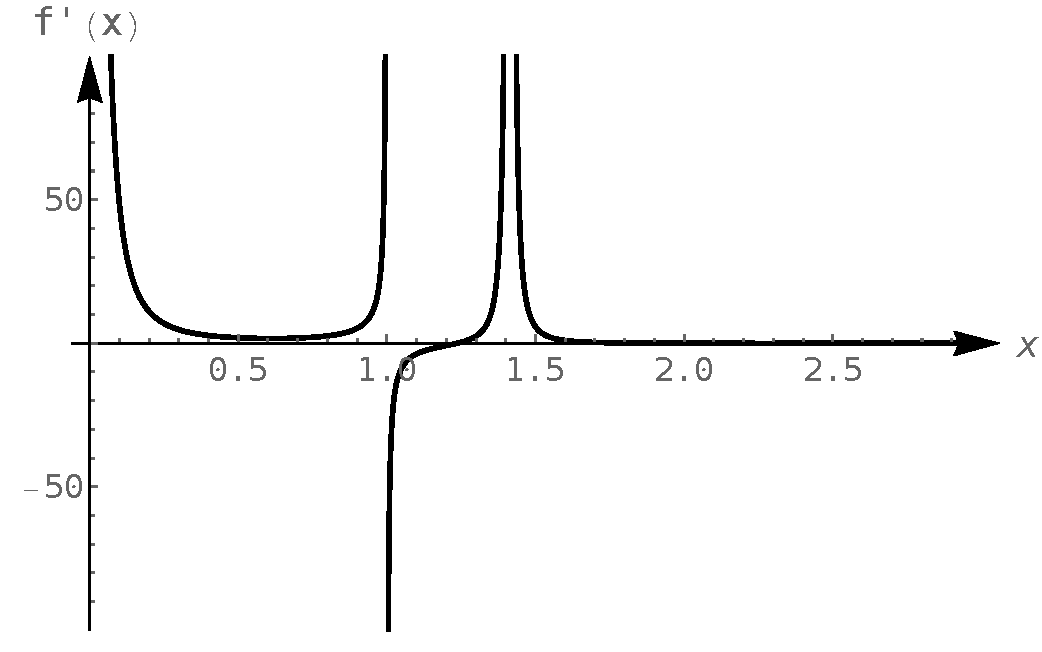
\includegraphics[width=0.40\textwidth]{functieonderzoek1L}}
\hspace*{0.5cm}
\subfigure[\label{functieonderzoek1S}]{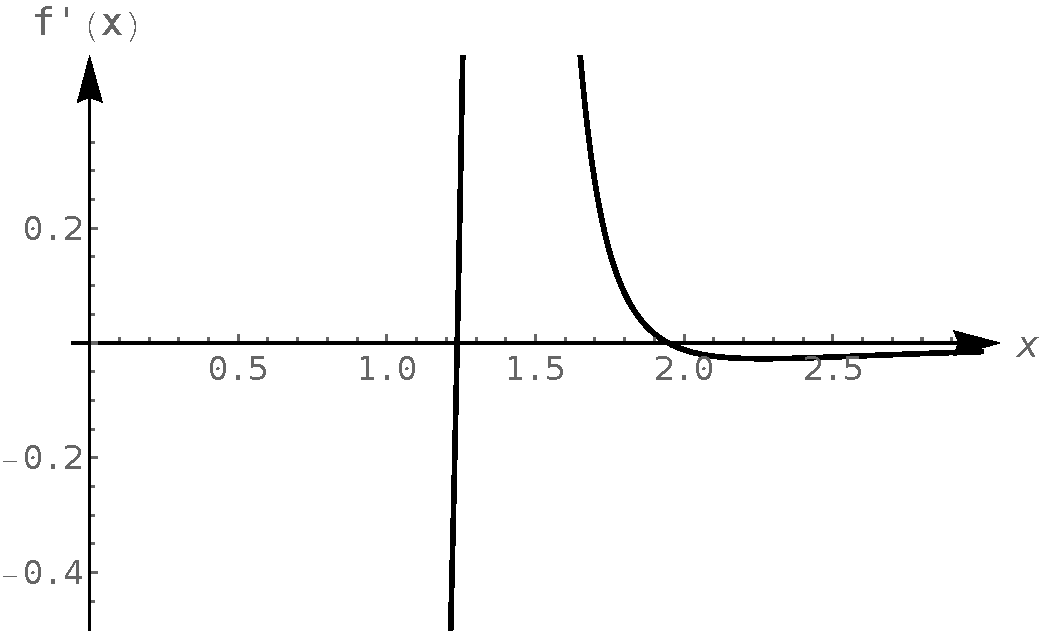
\includegraphics[width=0.40\textwidth]{functieonderzoek1S}}
}
\centerline{
\subfigure[\label{functieonderzoek2L}]{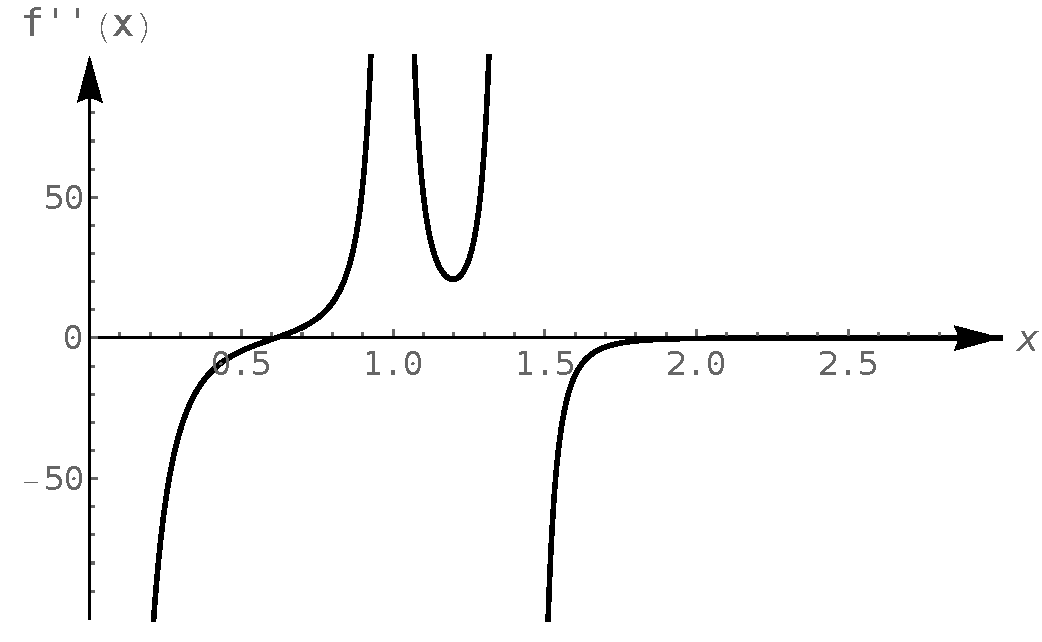
\includegraphics[width=0.40\textwidth]{functieonderzoek2L}}
\hspace*{0.5cm}
\subfigure[\label{functieonderzoek2S}]{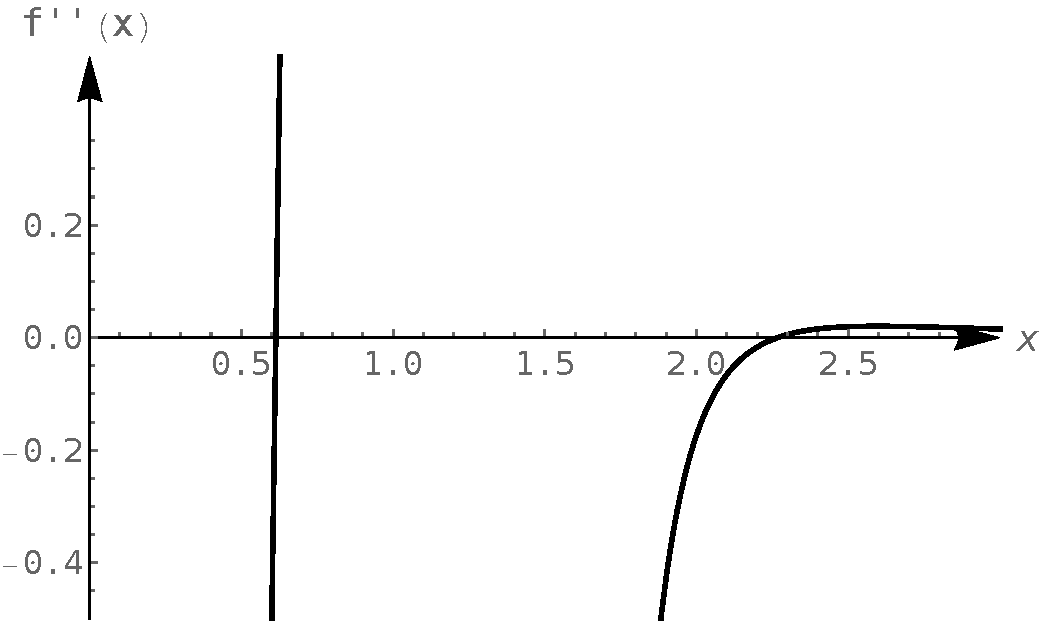
\includegraphics[width=0.40\textwidth]{functieonderzoek2S}}
}
\caption{\label{functieonderzoek}}
\end{figure}
\EndCurrentQuestion
\end{Exercise}

\begin{Answer}

\Question $\dom{\;f} = ]- \infty, - \sqrt{2}[ \, \cup \, ]- \sqrt{2}, -1[\,   \cup \,  ]1, \sqrt{2}[ \,  \cup \,  ]\sqrt{2}, + \infty[$
\Question $f$ is odd.
\Question $x = \pm \sqrt{e}$
\Question There are four vertical asymptotes: $x=\pm 1$ and $x= \pm \sqrt{2}$ (boundary points of the domain). There are two horizontal asymptotes $y=0$ for $x$ going to positive and negative infinity.
\Question $f$ descreases on $]1, 1.2[$ en $]1.9, 3]$ and increases on $]1.2, 1.9[$. At $x=1.2$ a minimum is reached and at $x=1.9$ a maximum is reached. On $]1, 1.5[$, $f$ is convex and on $]1.5, 3[$ it is concave.

\end{Answer}


\begin{Exercise} %{\bf (2p)} 
Construct up the integral to calculate the volume of solid of revolution obtained by rotating the region within $x^2+y^2=2$ AND within $(x-1)^2+y^2=1$ about the line with equation $x=2$.
\end{Exercise} 

\begin{Answer}


\Question With slices\\
$V = \pi \displaystyle \int\limits_{-1}^{1} \left(1+\sqrt{1-y^2} \right)^2 dy - \pi \displaystyle \int\limits_{-1}^{1} \left(2-\sqrt{2-y^2} \right)^2 dy = \pi \displaystyle \int\limits_{-1}^{1} \left(-4 + 2\sqrt{1-y^2} +4\sqrt{2-y^2} \right) dy$ 

\Question With cylindrical shells \\
$V = 4 \pi \displaystyle \int\limits_{0}^{1}  \sqrt{2x-x^2} (2-x) \, dx - 4 \pi \displaystyle \int\limits_{1}^{\sqrt{2}}  \sqrt{2-x^2} (2-x) \, dx $


\end{Answer}


\begin{Exercise} %{\bf (2p)} 
Consider the curve in $\mathbb{R}^3$ parameterised as
$$\vec{r}(t)=\left( 2t,3\sin \left( {2t} \right),3\cos \left( {2t} \right) \right)\,.$$
At what point in $\mathbb{R}^3$ do we arrive after traveling a distance of $\sqrt{10}\pi/3$ along this curve?
%  \url{http://tutorial.math.lamar.edu/Classes/CalcIII/VectorArcLength.aspx} 
\end{Exercise}

\begin{Answer}\phantom{}
We are in the point $\vec{r} \left(\dfrac{\pi \sqrt{10}}{3} \right) = \left(\dfrac{\pi}{3}, \dfrac{3 \sqrt{3}}{2}, \dfrac{3}{2}\right)$.
\end{Answer}


\begin{Exercise} %{\bf (2p)} 
Determine the parameter $p$ so that
$$
f(\mathbf{x})=\left(\sum\limits_{i=1}^{n}x_i^2\right)^p
$$
is a solution of 
$$
\sum\limits_{i=1}^{n}f_{x_ix_i}=0\,.
$$
\end{Exercise}

\begin{Answer}\phantom{}
$p=0 \quad \vee \quad p = \dfrac{-2n+4}{4} \; (n>0)$
\end{Answer}

\begin{Exercise} %{\bf (2p)} 
Consider a slab of negligible thickness with mass density $\delta(x,y,z)$ whose shape is described by $z=f(x,y)=\sqrt{x^2+y^2}$.
\Question Given the area of an infinitesimal particle of this plate in cartesian coordinates, i.e.
    $$
    dA=\sqrt{1+f_x^2+f_y^2}\,dx\ dy\,,
    $$
Determine a formula for the mass of this plate above a region $R$ in the $xy$ plane.
\Question Determine the mass of the plate for which $z=f(x,y)=\sqrt{x^2+y^2}$, $1\leq z\leq4$ en $\delta(x,y,z)=x^2z$.
\EndCurrentQuestion
\end{Exercise}

\begin{Answer}

\Question $M = \displaystyle \int\int \limits_{R} \delta \left(x,y,f(x,y)\right) \sqrt{1+f_x^2+f_y^2}\,dx\ dy$
\Question $M = \dfrac{1023 \pi \sqrt{2}}{5}$

\end{Answer}

\begin{Exercise} %{\bf (2.5p)} 
Cats have a very sensitive sense of smell that allows them to detect prey. During the hunt they typically follow the path along which the concentration of odour molecules increases the most. The cats Kamu and Kamiel are in their garden where the concentration of odour molecules is given by
$$
z=f(x,y)=e^{\cos(x)-y^2}\,.
$$
\Question Is the function $f$ bounded or unbounded?
\Question Suppose that Kamu and Kamiel are at the point $(x,y)=(3\pi/2,1)$ at the start of the hunt. In which direction will they then move?
\Question What is the rate at which the concentration of odour molecules increases in the direction determined under (b)?
\Question Determine the rule of the implicit function $F(x,y)=0$ that describes the traveled hunting trajectory.
\Question Does $F(x,y)=0$ define an explicit function $y=g(x)$ in the neighbourhood of $(x,y)=(3\pi/2,1)$?
\Question If possible, determine $y=g(x)$.
\EndCurrentQuestion
\end{Exercise}

\begin{Answer}

\Question $f(x,y) \in \, ]0,e]$, so $f$ is bounded.
\Question $\vec{\nabla} f \left(3\pi/2,1\right) = e^{-1} (1,-2)$
\Question $||\vec{\nabla} f \left(3\pi/2,1\right)|| = e^{-1} \sqrt{5}$
\Question $F(x,y) = \ln |y| - \ln \left| \dfrac{\cos(x) - 1}{\cos(x) + 1} \right|$
\Question Yes, because $\dfrac{\partial F}{\partial y} = \dfrac{1}{|y|} \stackrel{\left(3\pi/2,1\right)}{=} 1 \neq 0$
\Question $y = \dfrac{\cos(x) - 1}{\cos(x) + 1}$

\end{Answer}


\begin{Exercise} %{\bf (1p)} 
Consider the graph of the function $f(x,y)$ on the region \linebreak $[-2,2]\times[-2,2]$ in Figure~\ref{potentiaalfunctie}. \label{vraag_potentiaalfunctie}
	 \begin{figure}[H]
		\centering
		%\raisebox{0.5cm}{
		\centerline{
			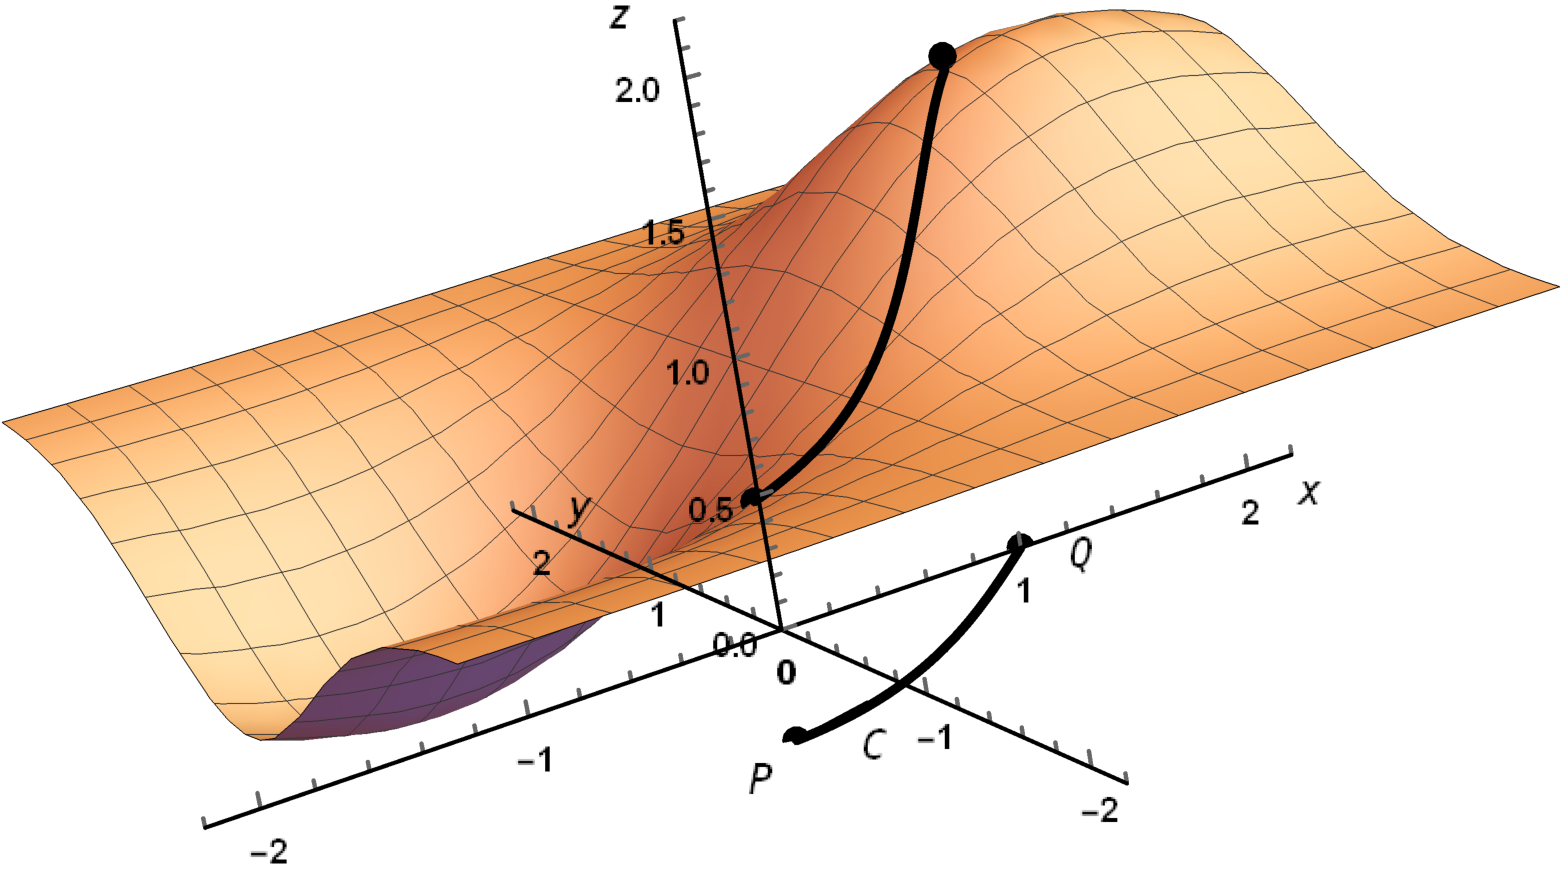
\includegraphics[width=0.50\textwidth]{potentiaalfunctie.pdf}
		}
		\caption{Graph of the function $f(x,y)$ from Question~\ref{vraag_potentiaalfunctie}.}
		\label{potentiaalfunctie}
	\end{figure}
Circle the correct statement.

\Question At the point $P(-0.5,-1)$ it holds that
    \begin{multicols}{3}
    \begin{enumerate}
    \item[(i)] $\dfrac{\partial f}{\partial y}>0$\,,
    \item[(ii)] $\dfrac{\partial f}{\partial y}=0$\,,
    \item[(iii)] $\dfrac{\partial f}{\partial y}<0$\,.
    \end{enumerate}
    \end{multicols}
\Question At the point $Q(1,0)$ it holds that
    \begin{multicols}{3}
    \begin{enumerate}
    \item[(i)] $\dfrac{\partial^2 f}{\partial x^2}>0$\,,
    \item[(ii)] $\dfrac{\partial^2 f}{\partial x^2}=0$\,,
    \item[(iii)] $\dfrac{\partial^2 f}{\partial x^2}<0$\,.
    \end{enumerate}
    \end{multicols}
\Question The line integral $\displaystyle\int_Cf(s)ds$ is
    \begin{multicols}{3}
    \begin{enumerate}
    \item[(i)] strictly positive,
    \item[(ii)] zero,
    \item[(iii)] strictly negative.
    \end{enumerate}
    \end{multicols}
\Question The vector field $\vec{\nabla}\,f$ is shown in
    \begin{multicols}{4}
    \begin{enumerate}
    \item[(i)] Figure~\ref{vectorveld1},
    \item[(ii)] Figure~\ref{vectorveld2},
    \item[(iii)] Figure~\ref{vectorveld3},
    \item[(iv)] Figure~\ref{vectorveld4}.
    \end{enumerate}
    \end{multicols}


\begin{figure}[H]
\centering

\centerline{
\subfigure[\label{vectorveld1}]{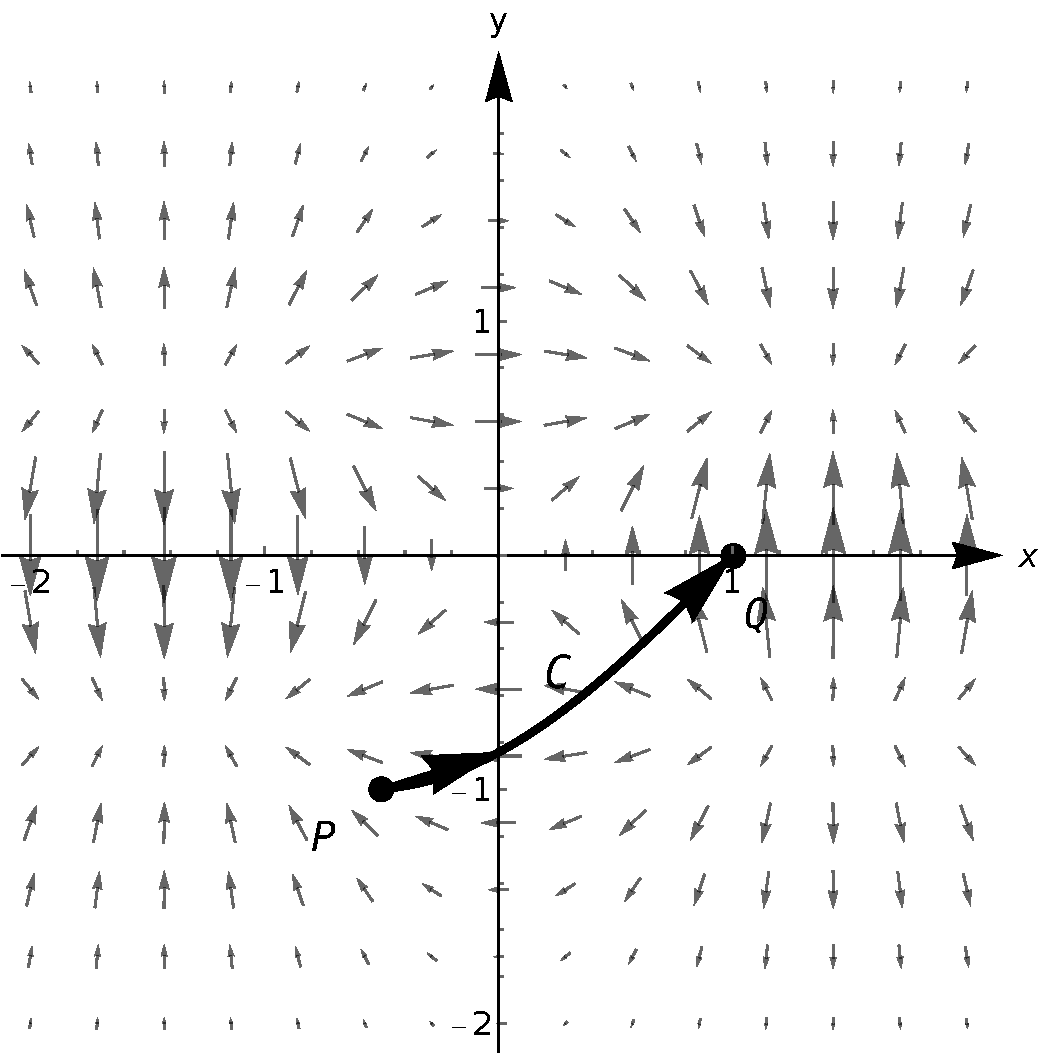
\includegraphics[width=0.45\textwidth]{Vectorveld3}}
\hspace*{0.5cm}
\subfigure[\label{vectorveld2}]{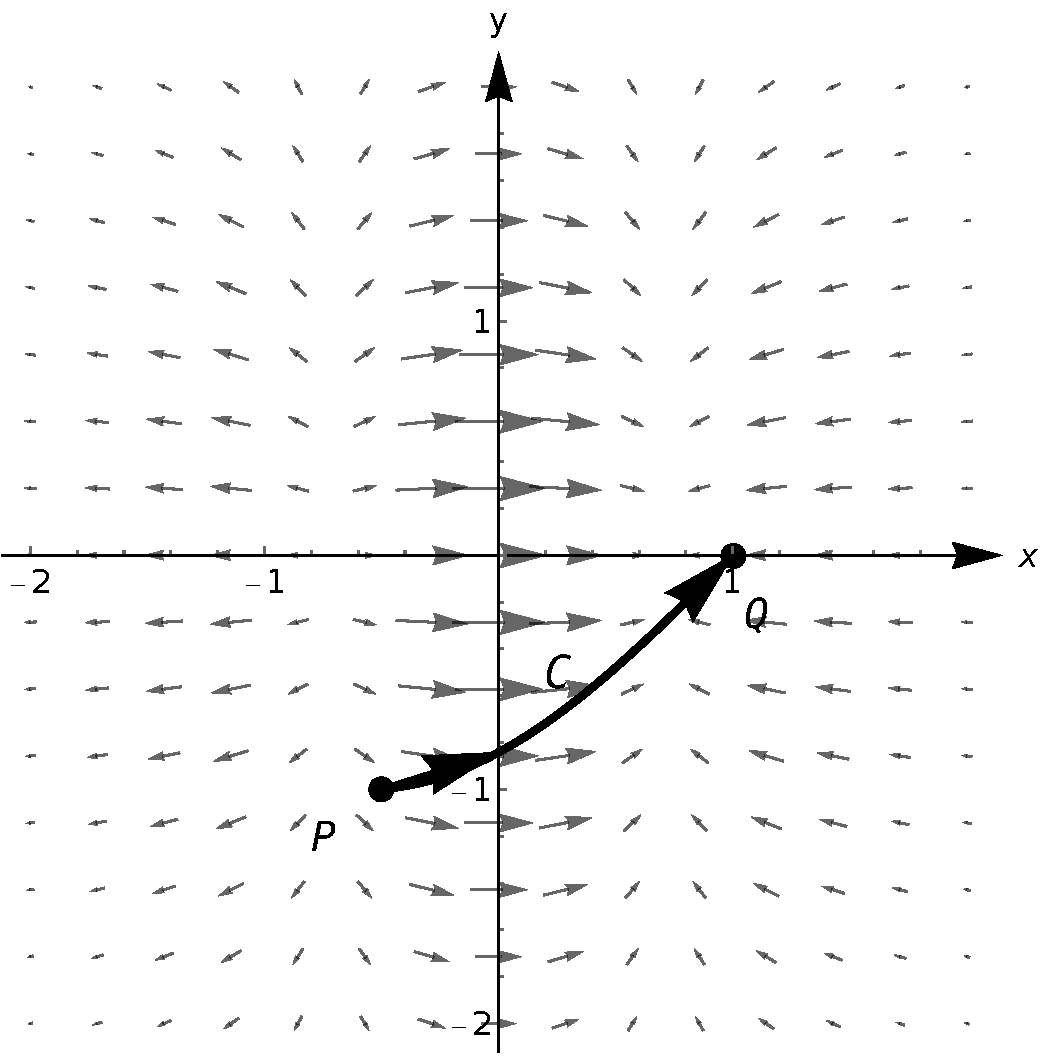
\includegraphics[width=0.45\textwidth]{Vectorveld4}}
%\hspace*{0.5cm}
%\subfigure[]{\includegraphics[width=0.33\textwidth]{parametric_eq_6-c}}
}
\centerline{
%\subfigure[]{\includegraphics[width=0.32\textwidth]{parametric_eq_5-d}}
%\hspace*{0.5cm}
\subfigure[\label{vectorveld3}]{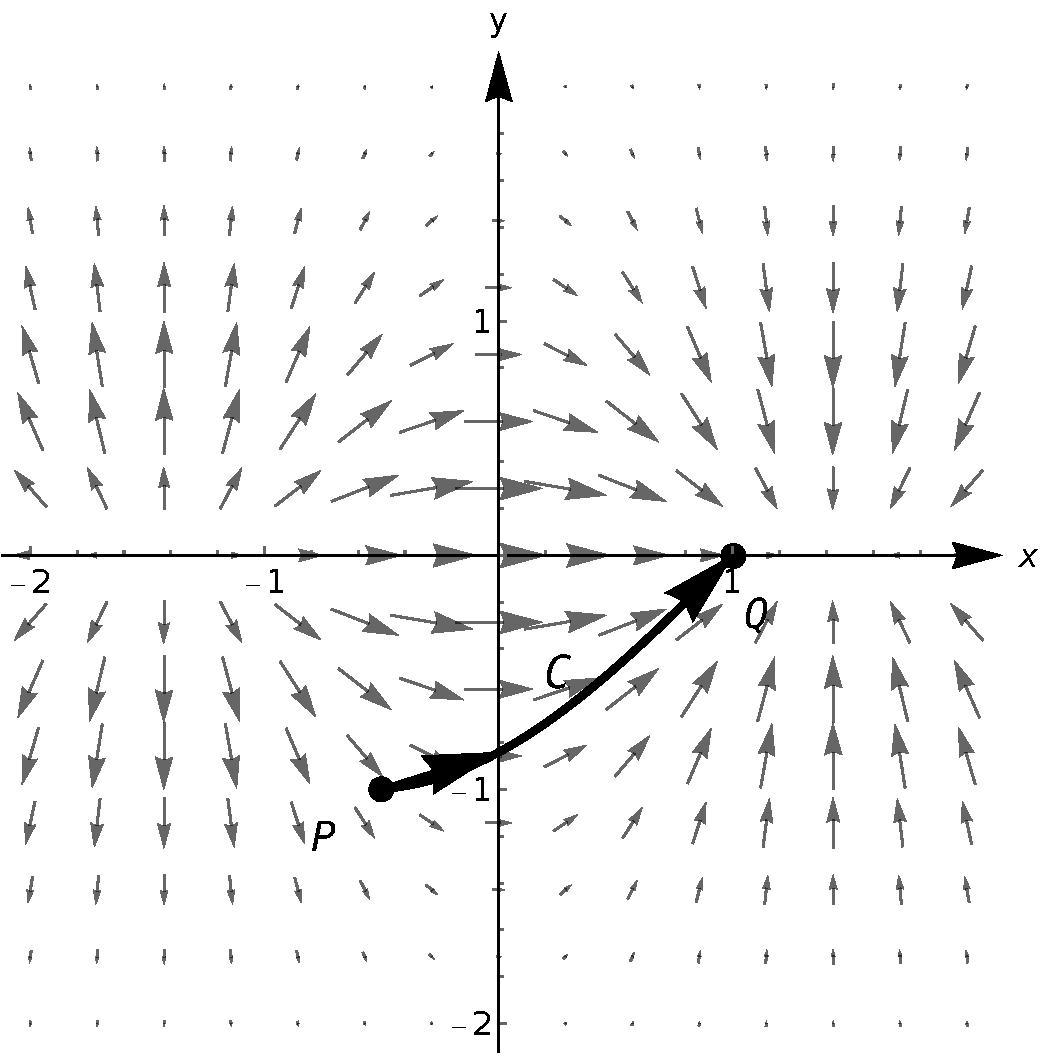
\includegraphics[width=0.45\textwidth]{Vectorveld1}}
\hspace*{0.5cm}
\subfigure[\label{vectorveld4}]{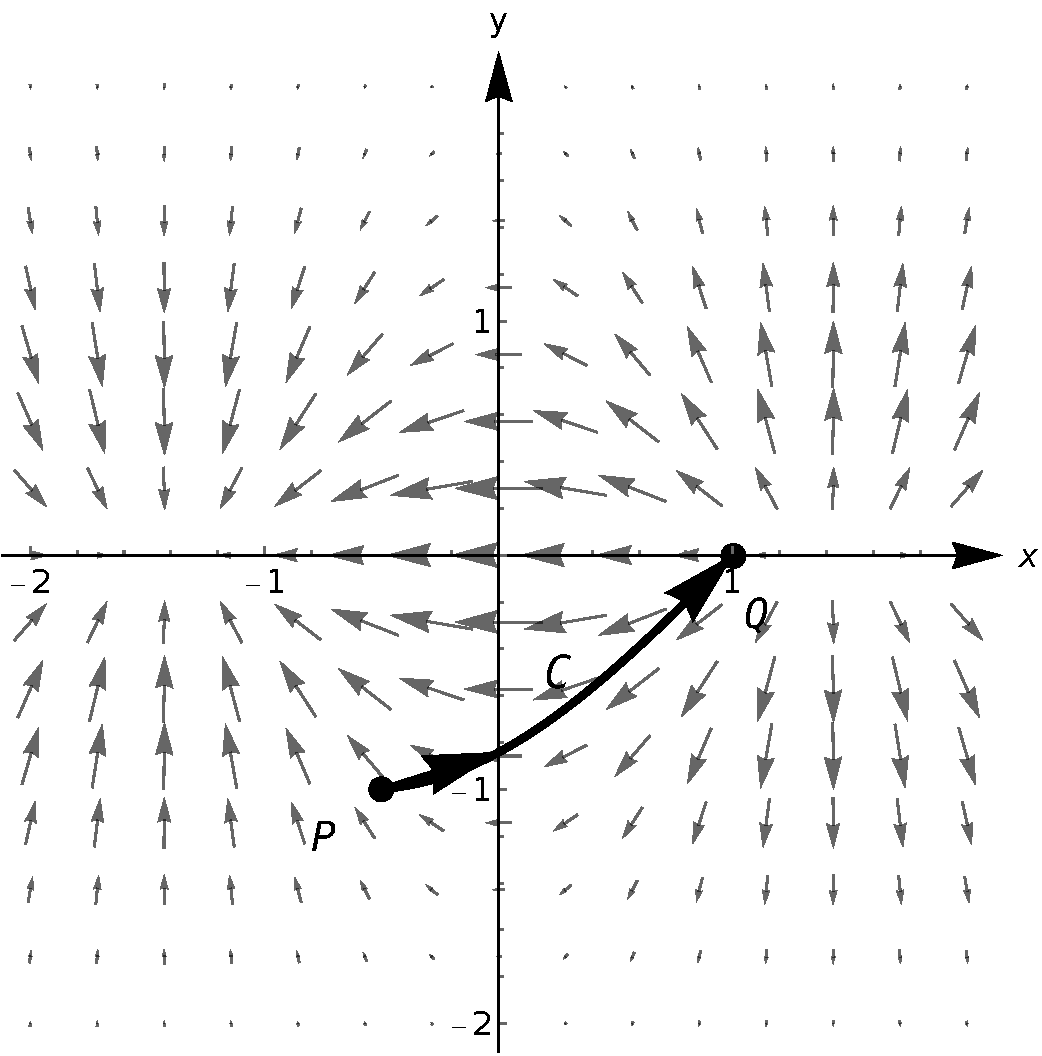
\includegraphics[width=0.45\textwidth]{Vectorveld2}}
}
\caption{\label{vectorvelden}}
\end{figure}
\EndCurrentQuestion
\end{Exercise} 

\begin{Answer}
\begin{multicols}{2}

\Question $\dfrac{\partial f}{\partial y}<0$
\Question $\dfrac{\partial^2 f}{\partial x^2}<0$
\Question strictly positive
\Question Figure~\ref{vectorveld3},
 \EndCurrentQuestion
\end{multicols}
\end{Answer}




%%%%%%%%%%%%%%%%%%%%%%%%%%%
%Examen augustus 2020
%%%%%%%%%%%%%%%%%%%%%%%%%%%
\section{Exam August 2020}

\begin{Exercise} %{\bf (1p)} 
Suppose
$$|f(x)-f(y)|\leq|x-y|^n$$ 
where $x,y\in\mathbb{R}$ and $n>1$. Prove that $f$ is a constant function.
\end{Exercise} 

\begin{Answer}\phantom{}
Prove this yourself.
\end{Answer}


\begin{Exercise} %{\bf (3.5p)} 
Consider the real-valued function $f$:
$$
f(x)=\csc(x)-2\sin(x).
$$
\Question Determine the domain and image of $f$.
\Question Determine the periodicity of $f$.
\Question Determine the symmetry of $f$.
\Question Determine all roots of $f$.
\Question Determine the asymptotes of $f$.
\Question Determine the extrema and inflection points of $f$.
\Question Examine the behavior of $f$ and sketch its graph.
\EndCurrentQuestion
\end{Exercise}

\begin{Answer}

\Question  $\dom{\;f} = ]0, \pi [ \,  + \,  k \pi, k \in \mathbb{Z}$
\Question The function is periodic with period $2 \pi$.
\Question The function is odd.
\Question $f(x) = 0 \quad \Leftrightarrow \quad x = \dfrac{\pi}{4} + k \pi, k \in \mathbb{Z} \quad \vee \quad x = \dfrac{3\pi}{4} + k \pi, k \in \mathbb{Z}$
\Question There are only vertical asymptotes at $x=k \pi, k \in \mathbb{Z}$.
\Question The extrema are found at $x = \dfrac{\pi}{2} + k \pi, k \in \mathbb{Z} $. There are no inflection points. 
\Question Onderzoek zelf het gedrag van $f$ en maak een schets. 

\end{Answer}


\begin{Exercise} % {\bf (2p)} 
Calculate the volume of the solid of revolution resulting from the rotation of the region enclosed by $y=0$, $y=x$, $xy=9$ and $x+y=10$ for $x\geq y$ about the $ y$ axis. 
\end{Exercise}

\begin{Answer}\phantom{}
With cylindrical shells: \\

$V = 2 \pi \displaystyle \int \limits_0^3 x^2 \, dx + 2 \pi \displaystyle \int \limits_3^9 9 \, dx + 2 \pi \displaystyle \int \limits_9^{10} x(10-x) \, dx = \dfrac{406 \pi}{3}$
\end{Answer}

\begin{Exercise} %{\bf (3p)} 
Determine the radius of convergence and the convergence interval of:
$$
\sum\limits_{n=1}^{+\infty}\dfrac{\ln(n+1)}{\sqrt{n}}\left(2x-3\right)^n\,.
$$
\end{Exercise}

\begin{Answer}\phantom{}
The convergence interval is $[1,2[$ and the radius of convergence is $1/2$.
\end{Answer}


\begin{Exercise} %{\bf (2.5p)} 
Consider the squeeze theorem for functions of $n$ variables.

\begin{theorem}[Generalised squeeze theorem]\label{thm:sqz2}
Let $f$, $g$ and $h$ be functions on an open ball $B$ in $\mathbb{R}^n$ containing the point $P=\mathbf{x}_0$ and for which it holds that
$$f(\mathbf{x})\leq g(\mathbf{x}) \leq h(\mathbf{x})$$ 
for all $\mathbf{x}$ in $B$. 

It then holds that
$$\lim_{\mathbf{x}\to \mathbf{x}_0} g(\mathbf{x}) = L$$ 
if
$$\lim_{\mathbf{x}\to \mathbf{x}_0} f(\mathbf{x}) = L = \lim_{\mathbf{x}\to \mathbf{x}_0} h(\mathbf{x})\,.$$
\end{theorem}

\Question Prove this theorem.
\Question Illustrate this statement and your proof with a sketch.
\Question Use this theorem to calculate the following limit:
    $$
    \lim_{(x,y)\to (0,0)} x^4\sin\left(\dfrac{1}{x^2+|y|}\right)\,.
    $$
\EndCurrentQuestion
\end{Exercise} 

\begin{Answer}\phantom{}
Prove this yourself.
\end{Answer}


\begin{Exercise} %{\bf (3p)} 
Consider the curve with polar equation $r(\theta)=\sin(\theta)\cos(\theta)$ whose graph is shown in Figure~\ref{Rose}.
\Question Construct the double integral to find the area $A_1$ of the region outside $r(\theta)=\sin(\theta)\cos(\theta)$ and inside $r=0.5$.
\Question Construct the double integral to determine the area $A_2$ of the region inside $r(\theta)=\sin(\theta)\cos(\theta)$ and outside $r=\sqrt{2}/4$. 
\Question Calculate $A_1$ \textit{or} $A_2$.
\EndCurrentQuestion
\begin{figure}[H]
\centering
%\raisebox{0.5cm}{
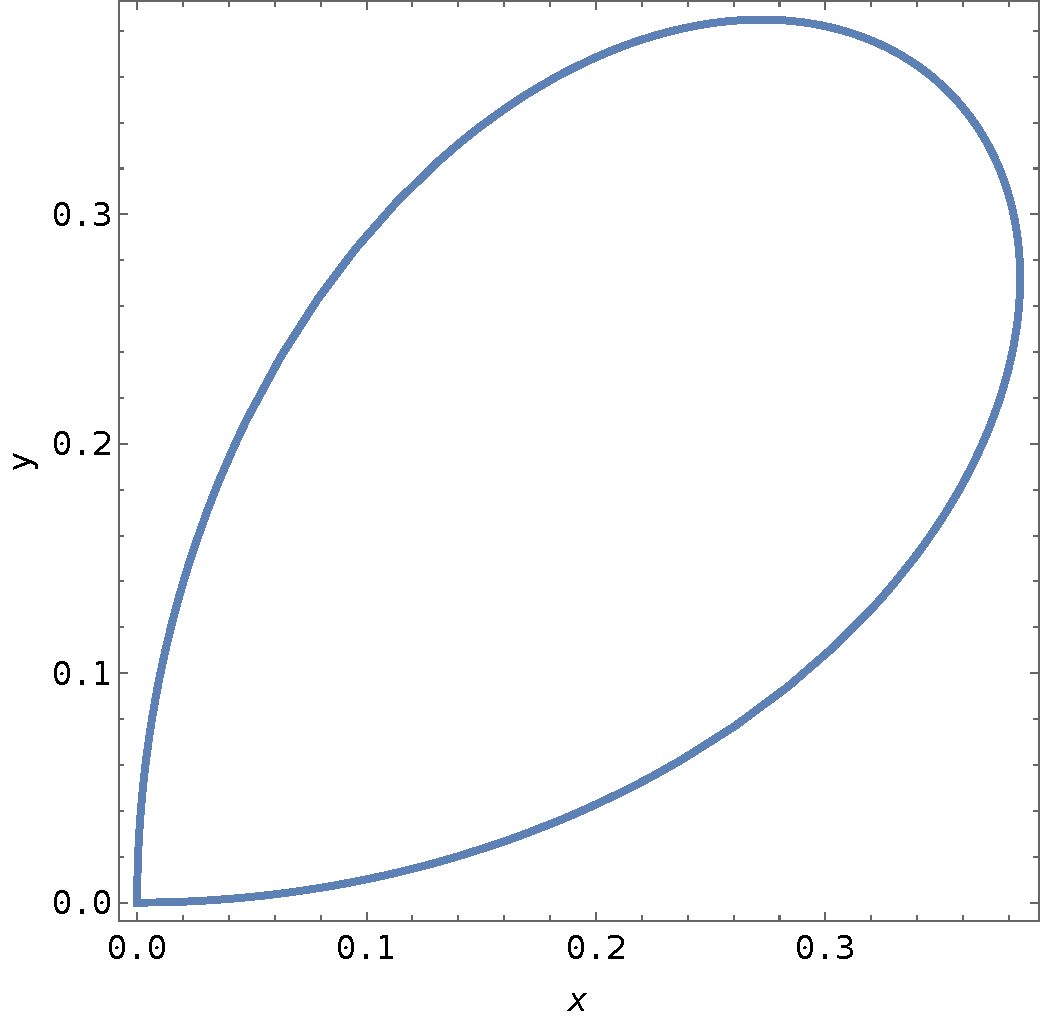
\includegraphics[width=0.5\textwidth]{Rose}
\caption{\label{Rose}}
\end{figure}
\end{Exercise} 

\begin{Answer}
\Question $A_1 = 2 \displaystyle \int \limits_0^{\pi/4} \int \limits_{1/2 \sin(2 \theta)}^{1/2} r \, dr d \theta$
\Question $A_2 = 2 \displaystyle \int \limits_{\pi/8}^{\pi/4} \int \limits_{\sqrt{2}/4}^{1/2 \sin(2 \theta)} r \, dr d \theta$
\Question $A_2 = \dfrac{1}{32}$

\end{Answer}

\begin{Exercise} %{\bf (2p)} 
Calculate the line integral on the \textit{conservative} vector field $\vec{F}\left(\frac{1}{x^2+1},2yz,y^2\right)$ along the curve $C$ with parameterisation $(t,2t,\arcsin(t))$ for $t\in[0,1]$ .
\end{Exercise} 

\begin{Answer}\phantom{}
$\displaystyle \oint_C \vec{F} \cdot d\vec{r} = f(B) - f(A) = \dfrac{9 \pi}{4}$
\end{Answer}


%%%%%%%%%%%%%%%%%%%%%%%%%%%
%Examen januari 2021
%%%%%%%%%%%%%%%%%%%%%%%%%%%
\section{Exam January 2021}

\begin{Exercise} %{\bf (2p)} 
The proportion of the population $p$ that adheres to the corona measures is described by:
$$
p(t)=\dfrac{e^{\beta_0+\beta_1(t-t^*)}}{1+e^{\beta_0+\beta_1(t-t^*)}}\,,
$$
where $t$ represents the time in days, $t^*>0$ the day on which measures take effect and $\beta_0>0$ and $\beta_1>0$ parameters. These parameters influence the time instant when we transition from an increase in the acceptance of the measures with increasing speed to an increase with decreasing speed, i.e. the inflection point of the graph of $p(t)$. The faster this time instant is reached, the more efficiently we can slow down the spread of the virus.  

Show that awareness campaigns to expedite this time instant should aim to increase $\beta_0$ or decrease $\beta_1$.
\end{Exercise} 

\begin{Answer}\phantom{}
You can check the impact of $\beta_i$ on the inflection point by using differentials. To do this, you must of course first find out the time instant at which the inflection point manifests itself. So you first calculate the second derivative. Then you determine for which $t_{BP}$ there is an inflection point. Finally, check the impact of $\beta_i$ on the inflection point by differentiating $t_{BP}$ with respect to $\beta_0$ and $\beta_1$.
\end{Answer}


\begin{Exercise} %{\bf (2p)}
If we use the $\epsilon$-$\delta$ definition of the limit in our definition for the continuity of a function of one variable $f$ in a point $c$, then we arrive at the following definition.

\begin{theorem}[Continuity in a point]\label{thm:con}
Let $I$ be an open interval and $c\in\,I$, then a function $f:I\to\mathbb{R}$ is continuous in the point $c$ if for all $\epsilon>0$ a $\delta>0$ exists such that $|f(x)-f(c)|<\epsilon$ if $|x-c|<\delta$ for all $x\in\,I$.
\end{theorem}

However, we can also define a stronger form of continuity.

\begin{theorem}[Uniform continuity]\label{thm:con2}
A function $f:I\to\mathbb{R}$ is uniformly continuous over $I$ if for all $\epsilon>0$ there exists a $\delta>0$ such that $|f(x)-f(y )|<\epsilon$ if $|x-y|<\delta$ for all $x,y\in\,I$.
\end{theorem}

\Question Explain what uniform continuity means.
\Question How does uniform continuity (Definition~\ref{thm:con2}) differ from continuity (Definition~\ref{thm:con})?
\Question Explain why uniform continuity implies continuity. 
\Question We know that $f(x)=x^2$ is continuous on its domain. Show that this function is not uniformly continuous on its domain.
\EndCurrentQuestion
% https://math.stackexchange.com/questions/653100/difference-between-continuity-and-uniform-continuity
% https://en.wikipedia.org/wiki/Uniform_continuity
\end{Exercise} 

\begin{Answer}\phantom{}
Show this yourself.
\end{Answer}

\begin{Exercise} %{\bf (2.5p)} 
Consider the real-valued function $f$:
$$
f(x)=\arccos{\left(\ln\left(x^2+1\right)\right)}.
$$
\Question Determine the domain and image of $f$.
\Question Examine the symmetry of $f$.
\Question Calculate the derivative $f'$. 
\Question How does $f'$ behave at the boundary points of the domain?
\Question Show that $f$ reaches a maximum on its domain.
\EndCurrentQuestion
\end{Exercise} 


\begin{Answer}

\Question $\dom{\;f} = \left[- \sqrt{e-1}, \sqrt{e-1}\right]$, \quad $\im{\;f} = \left[0, \dfrac{\pi}{2}\right]$
\Question The function is even.
\Question $f'(x) = \dfrac{-2x}{\left(x^2+1 \right) \sqrt{1 - \left(\ln(x^2+1)\right)^2}}$
\Question $f'\left( \pm \sqrt{e-1} \right) \rightarrow \mp \infty$. There is a vertical tangent to the graph of the function at the boundary points.
\Question The domain of the function is a closed interval. $f$ is also continuous on this interval. It follows from the extreme value theorem that $f$ reaches a maximum on its domain.

\end{Answer}


\begin{Exercise} % {\bf (1p)} 
Calculate the following integral:
$$
I = \int\limits\ln\left(x^2+2x+2\right)\,dx\,.
$$
\end{Exercise}

\begin{Answer}\phantom{}
$I = x \ln \left(x^2 + 2x + 2\right) - 2(x+1) + 2 \arctan (x+1) + \ln \left|(x+1)^2 + 1\right| + C$
\end{Answer}

\begin{Exercise} %{\bf (3p)} 
Consider the circle with equation $r=3\sin(\theta)$ and the cardioid with equation $r=1+\sin(\theta)$ shown in Figure~\ref{cirkelcardio}.

	 \begin{figure}[H]
		\centering
		%\raisebox{0.5cm}{
		\centerline{
			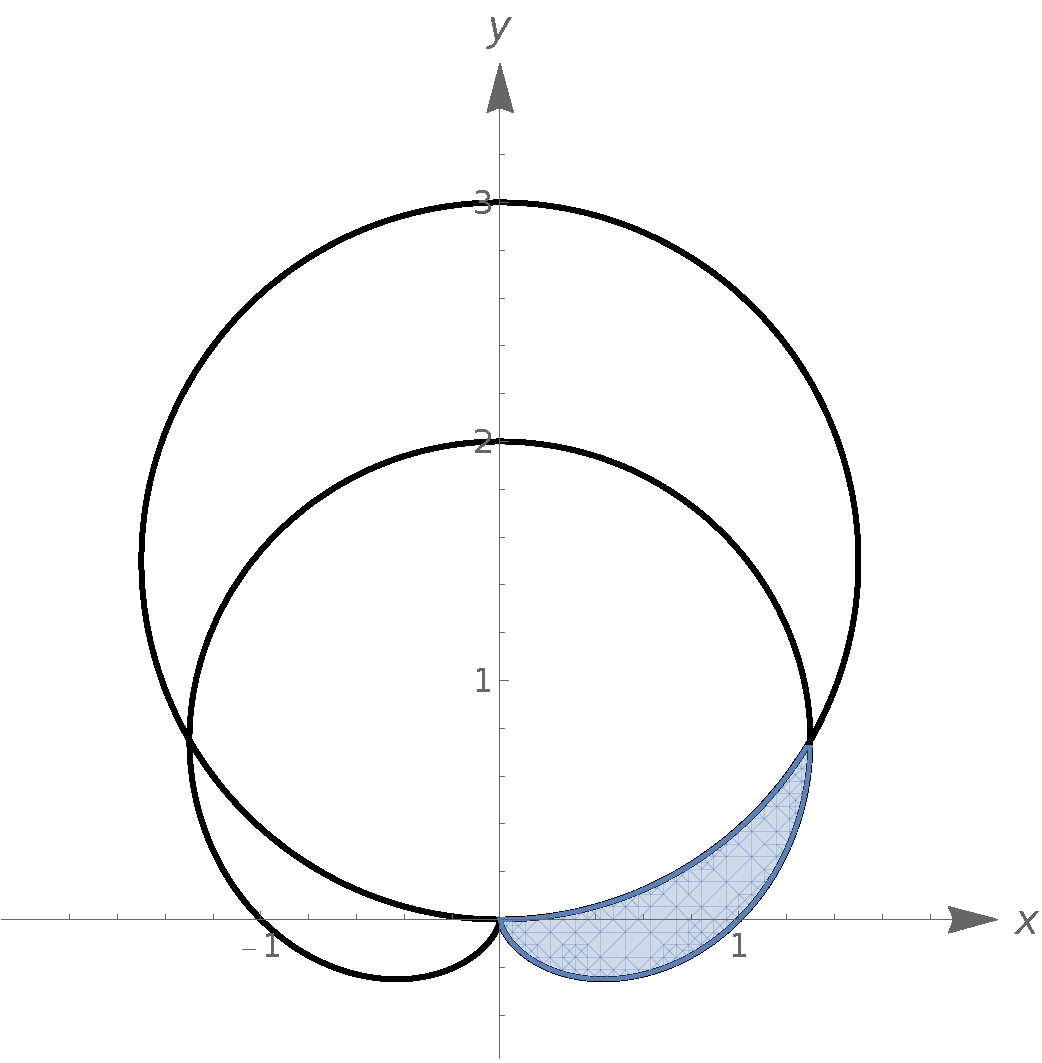
\includegraphics[width=0.4\textwidth]{cirkelcardio.pdf}
		}
		\caption{Graph of the circle $r=3\sin(\theta)$ and the cardioid $r=1+\sin(\theta)$.}
		\label{cirkelcardio}
	\end{figure}

\Question Construct the integral that allows you to calculate the area of the shaded region.
\Question Derive a formula for the volume of the solid of revolution obtained by rotating the area contained between the graphs of $r=f(\theta)$ and $\theta=0$ about the $x$ axis.
\Question Construct the integral that allows you to determine the volume of the solid of revolution resulting from rotation about the $x$-axis of the region enclosed by $r=3\sin(\theta)$, $y=0$ and $ x=3/2$.
\EndCurrentQuestion
\end{Exercise}

\begin{Answer}


\Question $A = \dfrac{1}{2} \displaystyle \int \limits_{-\pi/2}^{\pi/6}\left(1 + \sin (\theta) \right)^2 \, d \theta - \dfrac{1}{2} \displaystyle \int \limits_{0}^{\pi/6}\left(3\sin (\theta) \right)^2 \, d \theta$

\Question $V = \pi\displaystyle \int \limits_{\theta_1}^{\theta_2} r^2(\theta) \sin^2 (\theta) \left(r'(\theta) \cos(\theta) - r(\theta) \sin (\theta)  \right)  \, d \theta$

\Question $V = \pi\displaystyle \int \limits_{0}^{\pi/4} 9(\theta) \sin^4 (\theta) \left(3 \cos^2(\theta) - 3\sin^2 (\theta)  \right)  \, d \theta$
\end{Answer}


	
\begin{Exercise} %{\bf (1.5p)}  
The vector-valued functions below describe the paths of two flying insects.
\[ \vec{r}_1(t) = \left(t^2, 2t + 3, t^2 \right) \quad \text{ and } \quad  \vec{r}_2(t) = \left(5t-6, t^2,9 \right)  \]
\Question At what time instant will the insects collide?
\Question Where will the collision occur?
\Question Determine the angle between the paths at the point where the collision occurs.
\end{Exercise} 

\begin{Answer}
\Question The insects will collide at $t=3$.
\Question $\vec{r}_1(3) = \vec{r}_2(3) = (9,9,9)$
\Question The angle between the paths at the point where the collision occurs is $\arccos \left( \dfrac{21}{\sqrt{19} \sqrt{61}}\right) $.
\end{Answer}



\begin{Exercise} %{\bf (3p)} 
Given is the function of three variables:
$$
E(N,V,S)=\dfrac{3h^2N}{4\pi m}\left(\dfrac{N}{V}\right)^{2/3}e^{\left(\frac{2S}{3Nk}-\frac{5}{3}\right)}\,,
$$
where $h$, $m$ en $k$ are known constants. Now introduce the temperature via $T=\frac{\partial E}{\partial S}$ and the pressure via $p=-\frac{\partial E}{\partial V}$

\Question Show that 
    $$p(N,T,V)=\dfrac{kNT}{V}\,.$$
\Question Calculate $\vec{\nabla} p$.
\Question Calculate the directional derivative of $p$ in the direction determined by a directional vector of the line that is the intersection of $V=0$ and $N=T$.
\Question Consider the level surface $p=k$. Calculate the tangent plane to this level surface at the point $(1,1,1)$.
\EndCurrentQuestion
\end{Exercise} 


\begin{Answer}
\Question Show this yourself.
\Question $\vec{\nabla} p = \left(\dfrac{kT}{V}, \dfrac{kN}{V}, -\dfrac{kNT}{V^2}\right)$
\Question $D_{\vec{u}} p = \pm \dfrac{k(T+N)}{\sqrt{2} V}$
\Question $N+T-V = 1$
\end{Answer}


%%%%%%%%%%%%%%%%%%%%%%%%%%%
%Examen augustus 2021
%%%%%%%%%%%%%%%%%%%%%%%%%%%
\section{Exam Augustus 2021}

\begin{Exercise} %{\bf (2.5p)} 
Consider the real-valued function
$$
f(x)=\left\{
\begin{array}{rcl}
\dfrac{e^x-1}{|x|}\,,&&x\neq0\,,\\
1\,,&&x=0\,.
\end{array}\right.
$$

\Question Examine the continuity of $f$. Also specify where $f$ is left or right continuous.
\Question Classify any discontinuities.
\Question Calculate $f'(x)$ for all $x\neq0$. Is $f'(x)$ (strictly) positive or negative for $x>0$?
\Question Now, let $\text{dom}\,f=\mathbb{R}^+_0$. 
    \begin{enumerate}
        \item[(i)]  Why does the inverse function $f^{-1}$ exist on $]0,+\infty[$?
        \item[(ii)]  Calculate $\left(f^{-1}\right)'(e-1)$.
    \end{enumerate}
\EndCurrentQuestion
\end{Exercise}

\begin{Answer} 
\Question The function $f$ is continuous for all $x \neq 0$. $f$ is right continuous in $x=0$.
\Question There is a jump discontinuity at $x=0$.
\Question $f'(x) = \dfrac{e^x |x| - (e^x - 1) (\pm 1)}{x^2} = \left\{
\begin{array}{rcl}
\dfrac{e^x}{x} - \dfrac{e^x}{x^2} + \dfrac{1}{x^2} \,,& & x>0\,,\\[0.4cm]
-\dfrac{e^x}{x} + \dfrac{e^x}{x^2} - \dfrac{1}{x^2} \,,& & x<0\,.
\end{array}\right.$ \\

$f'$ is strictly positive for $x>0$.

\Question  
    \begin{enumerate}
        \item[(i)] Since $f'>0$ if $x>0$, $f$ is strictly increasing if $x>0$ and thus is injective for these $x$ values. Therefore the inverse function $f^{-1}$ exists on $]0,+\infty[$.
        \item[(ii)]  $\left(f^{-1}\right)'(e-1) = 1$.
    \end{enumerate}
\end{Answer}


\begin{Exercise} %{\bf (2.5p)}
If we use the  ($\epsilon$,$\delta$) definition of the limit in our definition for the continuity of a function of one variable $f$ at a point $c$, we arrive at the following definition. 

\begin{theorem}[Continuity in a point]\label{thm:con3}
Let $I$ be an open interval and $c\in\,I$, then the function $f:I\to\mathbb{R}$ is continuous in the point $c$ if for every $\epsilon>0$ there exist a $\delta>0$ such that $|f(x)-f(c)|<\epsilon$ if $|x-c|<\delta$ for every $x\in\,I$.
\end{theorem}

However, we can also define an alternative form of continuity. 

\begin{theorem}[Lipschitz continuity]\label{thm:con4}
A function $f:I\to\mathbb{R}$ is Lipschitz continuous on $I$ if there exists a number $L$ such that for all $x,\,y\in\mathbb{R}$ it holds true that 
$$
|f(x)-f(y)|\leq L|x-y|\,. 
$$
The smallest number $\displaystyle L$ for which this inequality holds true, is called the Lipschitz constant of $f$. 
\end{theorem}

\Question Explain what Lipschitz continuity means. 
\Question Wherein does Lipschitz continuity differ (Definition~\ref{thm:con4}) from continuity (Definition~\ref{thm:con3})?
\Question Show that the sine and consine functions are Lipschitz continuous and determine their Lipschitz constants.
\Question Give an example of a function that is over its domain
    \begin{enumerate}
        \item differentiable, but not Lipschitz continuous.
        \item not differentiable, but Lipschitz continuous.
    \end{enumerate}
\EndCurrentQuestion
\end{Exercise}

\begin{Answer}\phantom{}
Prove for yourself.

\end{Answer}

\begin{Exercise} %{\bf (3p)} 
Determine the volume of the body of revolution created by rotating the area within $x^2+y^2=2$ and within $(x-1)^2+y^2=1$ around the line $x=2$.
\end{Exercise} 

\begin{Answer}\phantom{}
Via shells: $V = 2 \displaystyle \int \limits_0^1 2 \pi (2-x) \sqrt{1 - (x-1)^2} \, dx + 2 \displaystyle \int \limits_1^{\sqrt{2}} 2 \pi (2-x) \sqrt{2-x^2} \, dx  =3 \pi^2 - 4 \pi$

\end{Answer}

\begin{Exercise} % {\bf (3p)} 
Determine the convergence radius and convergence interval of the power series below:
$$
\sum\limits_{n=1}^{+\infty}\dfrac{\ln(n+1)}{\sqrt{n}}(2x-3)^n
$$
Thoroughly motivate your decisions. 
\end{Exercise} 
The convergence interval is $[1,2[$. The convergence radius is $1/2$. 

\begin{Exercise} % {\bf (2.5p)}
A function $f:\mathbb{R}^n \rightarrow \mathbb{R}$  is called $f$ homogeneous of degree $p \in \mathbb{R}$ if 
\begin{equation}
\forall \vec{x} \in \mathbb{R}^n, \; \forall t>0: \quad f(t\vec{x}) = t^p f(\vec{x}).
\label{homogeen}
\end{equation}
Euler's homogeneous function theorem applies to such functions.

\begin{theorem}[Euler's homogeneous function theorem]\label{thm:euler}
If $f:\mathbb{R}^n \rightarrow \mathbb{R}$ is differentiable over $\mathbb{R}^n$, then it holds true that
$f$ is homogeneous of degree $p$ if and only if
\begin{equation}
\vec{x} \cdot \nabla f(\vec{x}) = p f(\vec{x}), \quad \forall \vec{x} \in \mathbb{R}^n.
\label{euler}
\end{equation}
\end{theorem}
\Question Prove the sufficient condition ($\Longrightarrow$).
\Question Complete the proof below for the necessary condition ($\Longleftarrow$). 
    
\vspace*{1cm} 
\textbf{Prove} Assume that eq.~\eqref{euler} holds true and choose $\vec{x}\in\mathbb{R}^n$ at random, but fixed. We define the following function:
$$
g(t) = f(t\vec{x}) - t^p f(\vec{x}),
$$
for all $t>0$. The theorem is proven if we can show that $g(t)~=~0$ for all $t>0$. 

Apparently $g(1) = 0$. Derivation to $t$ gives us:\\[0.25cm]
$$
g'(t) = \dotrule{0.80\textwidth}
$$
\\[0.2cm]
As $t \vec{x} \in\mathbb{R}^n$, for all $t>0$, applies to the understated
$$
(t\vec{x}) \cdot \nabla f(t\vec{x}) = pf(t\vec{x}),
$$
such that we can rewrite $g'(t)$ as a function of $g(t)$ if\\[0.25cm]
\begin{equation}
g'(t) =  \dotrule{0.70\textwidth}
\label{euler1}
\end{equation}
Next, we define the function $h$ as follows.:\\[0.25cm]
$$
g(t) = t^p h(t),
$$
for all $t>0$. Deriving the above relationship gives\\[0.25cm]
\begin{equation}
g'(t) =  \dotrule{0.70\textwidth}
\label{euler2}
\end{equation}

from which by equating Equations~\eqref{euler1} and \eqref{euler2} follows \\[0.25cm]
$$
 \dotrule{0.80\textwidth}
$$
\\[0.2cm]such that  \dotrule{0.82\textwidth}\vspace*{0.5cm}

\dotrule{0.90\textwidth}\vspace*{0.5cm}

\dotrule{0.90\textwidth}\vspace*{0.5cm}

\dotrule{0.90\textwidth}\vspace*{0.5cm}

\dotrule{0.90\textwidth}
\end{Exercise} 

\begin{Answer}\phantom{}
%%% BEWIJS INGEVULD
Assume that eq.~\eqref{euler} holds true and choose $\vec{x}\in\mathbb{R}^n$ at random, but fixed. We define the following function:
$$
g(t) = f(t\vec{x}) - t^p f(\vec{x}),
$$
for all $t>0$. The theorem is proven if we can show that $g(t) = 0$ for all $t>0$. 

Apparently $g(1) = 0$. Derivation to $t$ yields, again using the chain rule:
$$
g'(t) = \nabla f(t\vec{x}) \cdot \vec{x} - p t^{p-1} f(\vec{x}), \quad \forall t>0.
$$
As $t \vec{x} \in  \mathbb{R}^n$, $\forall t>0$, applies to understated
$$
(t\vec{x}) \cdot \nabla f(t\vec{x}) = pf(t\vec{x}),
$$
such that $g'(t)$ can be rewritten as
$$
g'(t) = \frac{1}{t} \left[ \nabla f(t\vec{x}) \cdot (t\vec{x}) - p t^p f(\vec{x}) \right] = 
\frac{p}{t} \left[ f(t \vec{x}) - t^p f(\vec{x}) \right] = \frac{p}{t} g(t), \quad \forall  t>0.
$$
Next, we define the function $h$ as follows:
$$
g(t) = t^p h(t), \quad \forall t>0.
$$
Deriving the above relationship gives
$$
g'(t) = t^p h'(t) + p t^{p-1} h(t),
$$
from which follows by equation 
$$
\frac{p}{t} g(t) = t^p h'(t) + \frac{p}{t} g(t), \quad \forall t>0,
$$
Such that we can conclude that $h'(t) = 0$, $\forall t>0$. Consequently, the function $h$ is constant and therefor there exists a number $c \in\mathbb{R}$ such that $g(t) = ct^p$, for all positive $t$.
However, since we already established that $g(1) = 0$, it must be that $c=0$, so that $g(t) = 0$, $\forall t>0$.
\end{Answer}



\begin{Exercise} %{\bf (1.5p)} 
Calculate the volume of the body located outside $x^2 + y^2 = 1$, inside $x^2 + y^2 =4$, under $z=\sqrt{x^2+y^2}$ and above $z=-\sqrt{x^2+y^2}$. %Heel kort met cilindercoördinaten! %Bio-irs
\end{Exercise} 
\begin{Answer}\phantom{}
$V = 2 \displaystyle \int \limits_1^2 \int \limits_0^{2 \pi} r^2 \, d \theta dr = \dfrac{28 \pi}{3} $

\end{Answer}


\begin{Exercise} %{\bf (1p)} 
In each case, perform the requested transformation without calculating the integral. 
\Question Rewrite the triple integral below using spherical coordinates.
$$
I_1=\displaystyle\int\limits_0^3\int\limits_0^{\sqrt{9-y^2}}\int\limits_{\sqrt{x^2+y^2}}^{\sqrt{18-x^2-y^2}}\left(x^2+y^2+z^2\right)\,dz\,dx\,dy
$$
\Question Rewrite
$$
I_2=\int_C xy dx+x^2y^3 dy
$$
as a double integral if $C$ is given by the triangle with vertices in $(0,0)$, $(1,0)$ and $(1,2)$ and $C$ is run through in a clockwise direction.
\EndCurrentQuestion
\end{Exercise} 
\begin{Answer}\phantom{}
\Question $I_1 = \displaystyle \int \limits_0^{\pi/2}  \int \limits_0^{\pi/4} \int \limits_0^{\sqrt{18}} \rho^4 \sin(\phi) \, d \rho d \phi d \theta $

\Question $I_2 = -\displaystyle \int \limits_0^{1}  \int \limits_0^{2x} \left( 2xy^3 - x \right) \, dy dx  = -\displaystyle \int \limits_0^{2}  \int \limits_{y/2}^{1} \left( 2xy^3 - x \right) \, dx dy$

\end{Answer}


\fi



%Einde Bio-irs
%%%%%%%%%%%%%%%%%%%%%%%%%%%%%%%%%%%




%%%%%%%%%%%%%%%%%%%%%%%%%%%%%%
%Industrieel ingenieurs
%%%%%%%%%%%%%%%%%%%%%%%%%%%%%%
\ifcalculus
%%%%%%%%%%%%%%%%%%%%%%%%%%%
%Examen Wiskunde I/A jan 2019
%%%%%%%%%%%%%%%%%%%%%%%%%%%
\section{Exam January 2019}
\begin{Exercise} For each statement, indicate whether it is True, False, or not verifiable based on the data provided. Also provide a brief rationale for your answer. 

\Question The function 
$$
f(x)=\dfrac{\sin^2(x)+\cos(x)}{\tan(x)\,\csc(x)}
$$
is not even.
% Fout
\Question It holds true that
$$
\cos\left(2\arcsin(x)\right)=1-2x^2\,.
$$
% juist
%Varberg 372
\Question If $x=f(t)$ and $y=g(t)$, then we can find a function $h$ for which it holds that $y=h(x)$.
% Varberg 552
% Fout
\Question For the circumference $O$ of the ellipse 
$$
\dfrac{x^2}{a^2}+\dfrac{y^2}{b^2}=1\,,
$$
where $b<a$, it holds that $2\pi\,b<O<2\pi\,a$.
% Juist
% Varberg
\Question For any two random vectors $\vec{u}$ and $\vec{v}$ it holds that
$$
|\vec{u}\cdot\vec{v}|\leq\|\vec{u}\|\|\vec{v}\|\,.
$$
% Juist
% Varberg 613
\Question All intersections of the graphs of $r=f(\theta)$ and $r=g(\theta)$ can be found by solving $f(\theta)=g(\theta)$.
% Fout
% Varberg 552

\Question If the radius of a spherical balloon being inflated increases at a rate of 3 mm per second, then the volume of the balloon increases at a rate of 27 mm$^3$ per second.
% Fout
% Varberg 148
\Question For an increasing function, the left Riemann sum is always smaller than the right Riemann sum.
% Juist
% Varberg 271


\Question If $f(x,y)=4x+4y$, then it holds true that
$$
\left|D_{\vec{u}}f(x,y)\right|\leq4\,.
$$
% Fout
% Varberg 673.
\end{Exercise}


\begin{Answer}\phantom{}

\Question False. The function is even, because $f(-x)=f(x)$
\Question True. This can be verified with the formula $\cos(2\alpha)=\cos^2(\alpha)-\sin^2(\alpha)$.
\Question False. For polar curves, this is not possible.
\Question True. It can be reasoned that a circle with radius $a$ has a larger circumference, because it is completely around the ellipse, and a circle with radius $b$ has a smaller circumference, because it is completely inside the ellipse.
\Question True. Can be shown via definition of scalar product.
\Question False. Sometimes the origin is not found, e.g. when $r_1=\sqrt{3}\cos(\theta)$ and $r_2=\sin(\theta)$.
\Question False. $V_t=12\pi r^2$.
\Question True. To be seen on figures with rectangles.
\Question False. It is true that $\left|D_{\vec{u}}f(x,y)\right|\leq 4\sqrt{3}$
  
\end{Answer}




\begin{Exercise} Determine which equation belongs to which graph in Figure~\ref{fig_test1_1}. 
\begin{multicols}{3}
\begin{enumerate}
\item[] 
\item[] 
\item[] 
\item[]
\item[(1)] $r(\theta)=1+\dfrac{\sin(\theta)}{2}$
\item[(2)] $\vec{r}(t)=\left(3 \sin(2 t), t, t\right)$
\item[(3)] $x(t)=\sin\left(t+\cos(t)\right)$ en\\ 
$y(t)=\cos\left(t+\sin(t)\right)$
\item[(4)] $r(\theta)=1+\dfrac{\cos(\theta)}{2}$
\item[(5)] $\vec{r}(t)=\left(t\cos( t), t\sin(t),t\right)$
\item[(6)] $\vec{r}(t)=\left(\cos( t), \ln(t), \sin(t)\right)$
\end{enumerate}
\EndCurrentQuestion
\end{multicols}
\begin{figure}[H]
\centering
%\raisebox{0.5cm}{
\centerline{
\subfigure[]{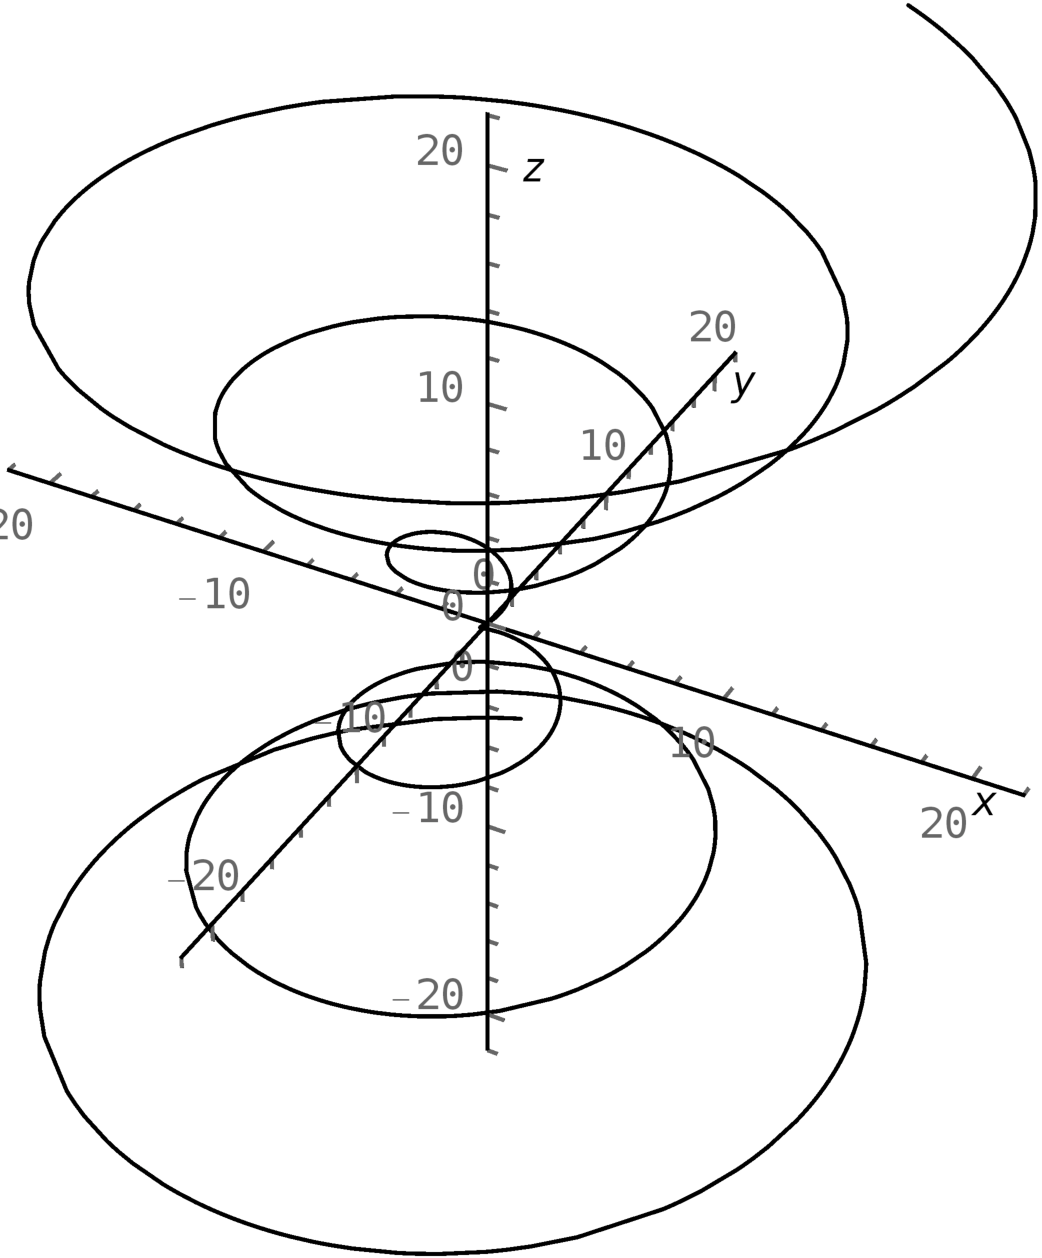
\includegraphics[width=0.3\textwidth]{fig_PGE_1a}}
%(-x,-y)
\hspace*{0.5cm}
\subfigure[]{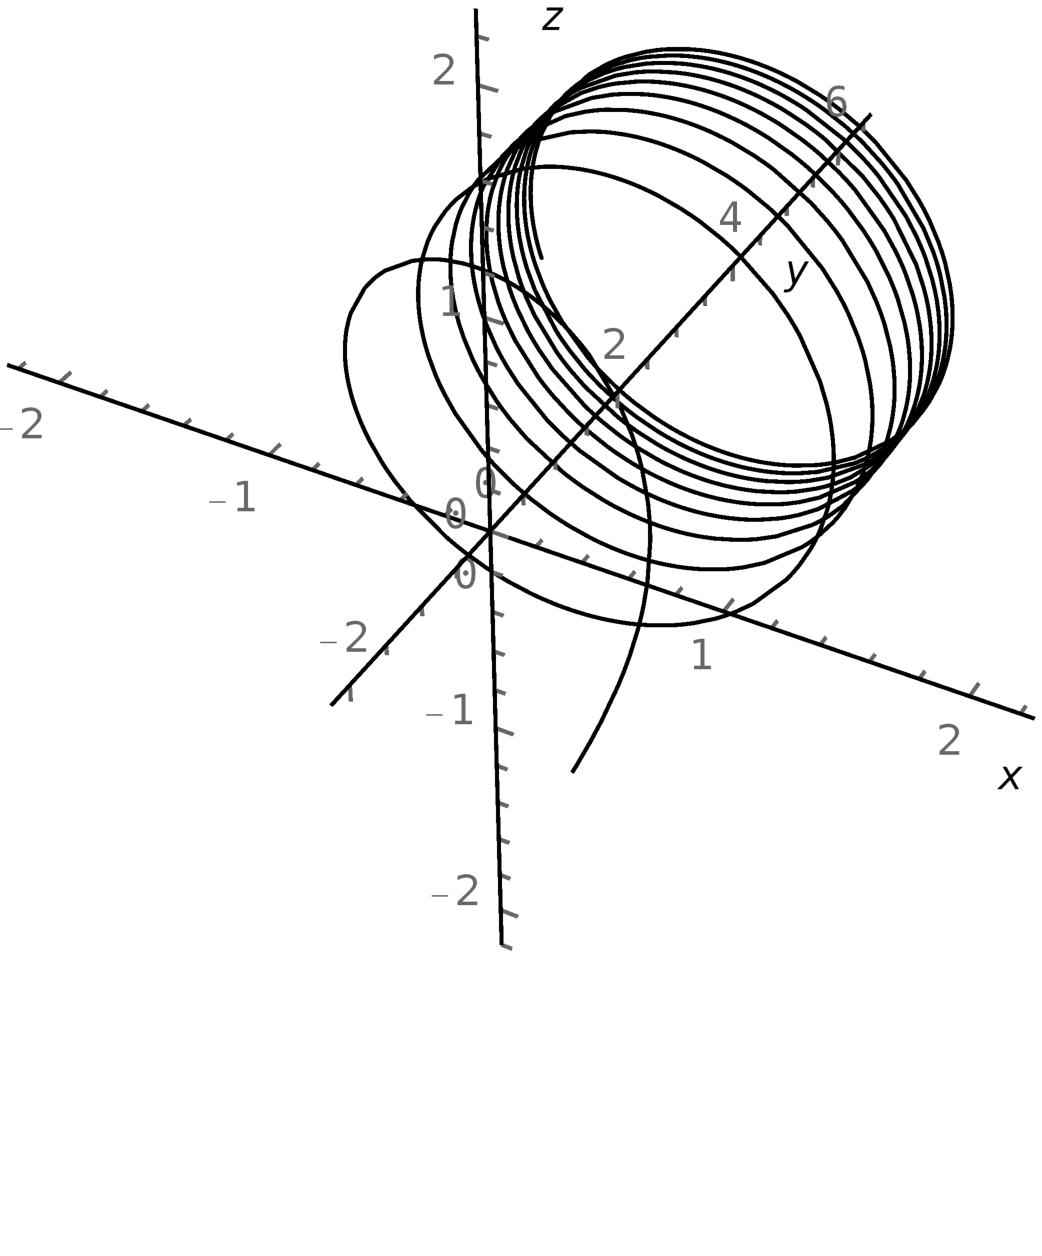
\includegraphics[width=0.33\textwidth]{fig_PGE_1b}}
\hspace*{0.5cm}
\subfigure[]{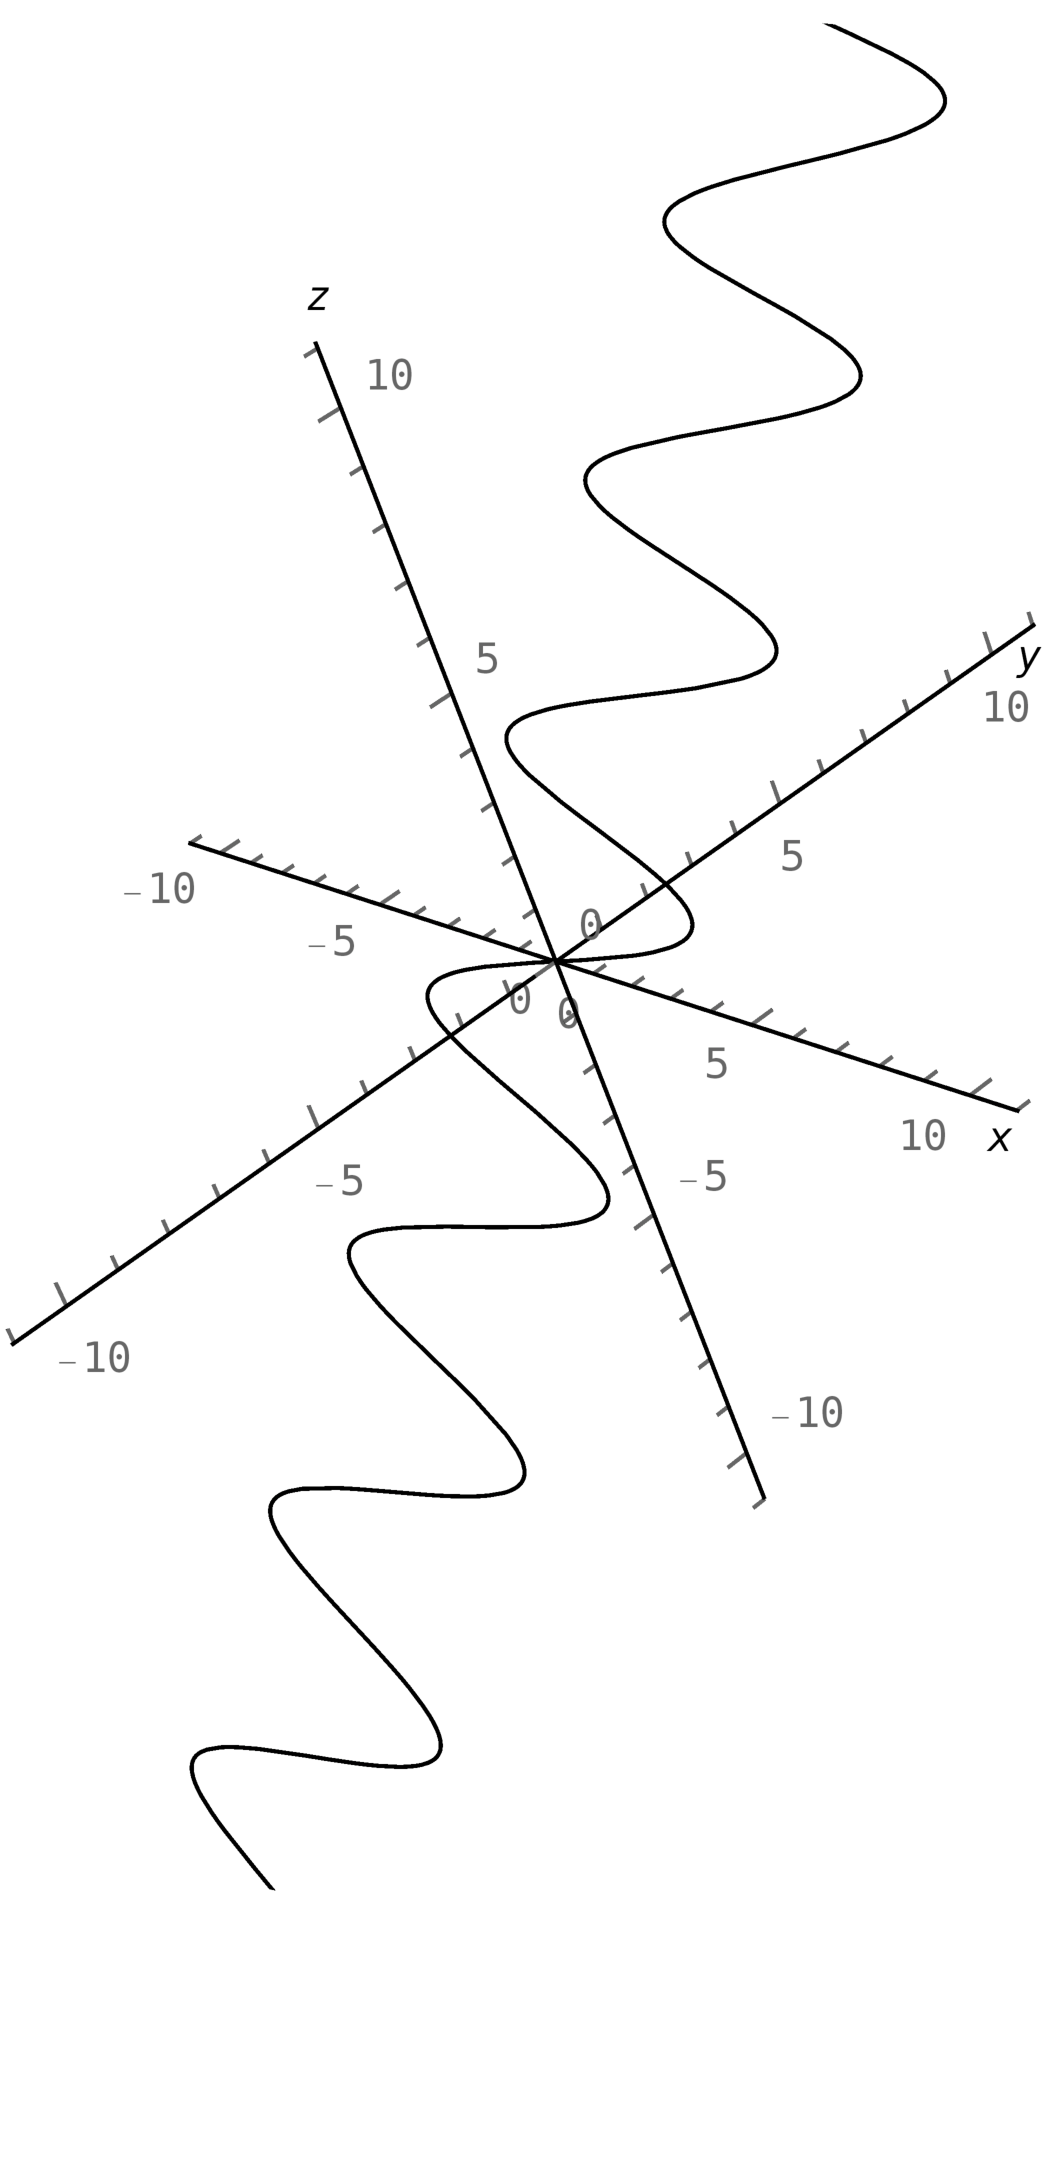
\includegraphics[width=0.18\textwidth]{fig_PGE_1c}}
%(0,x)
}
\centerline{
\subfigure[]{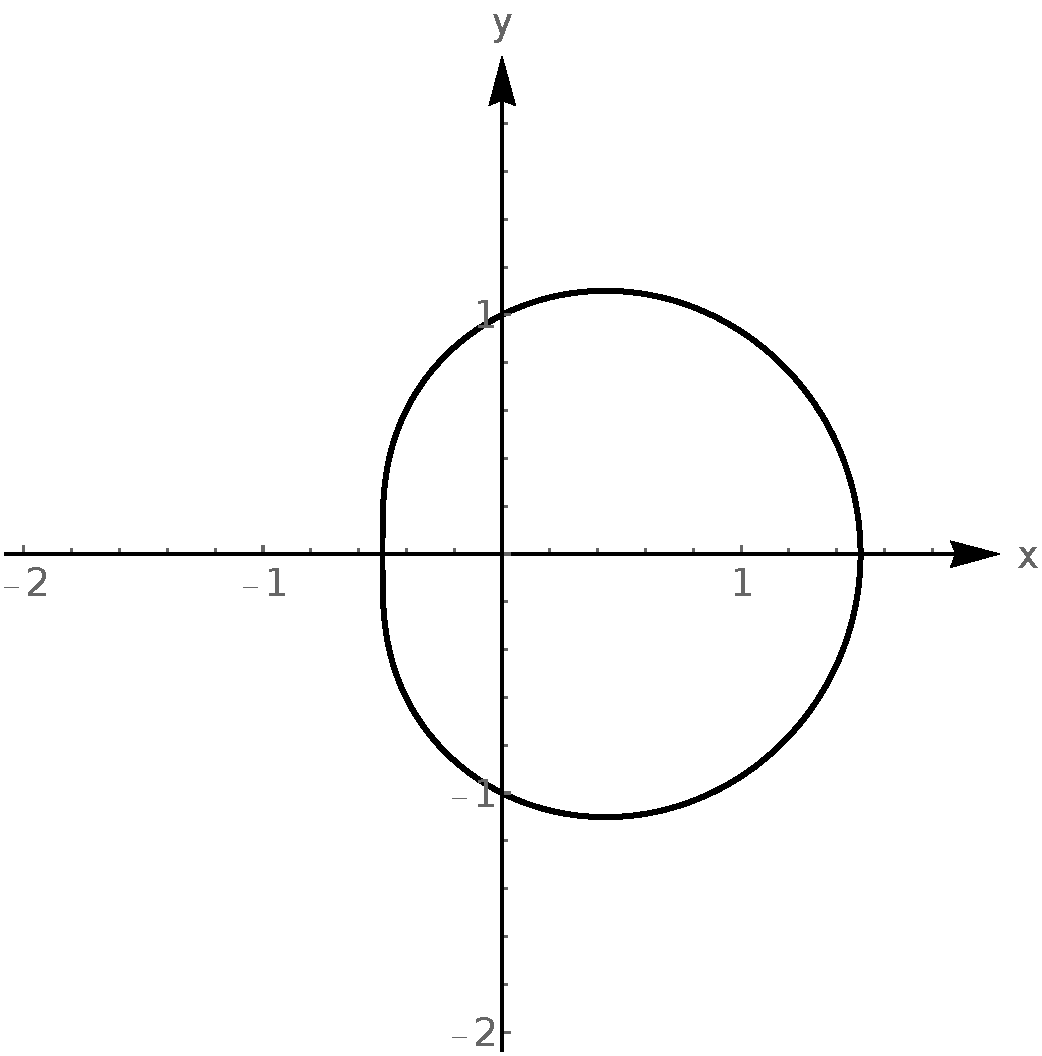
\includegraphics[width=0.33\textwidth]{fig_PGE_1d}}
\hspace*{0.5cm}
\subfigure[]{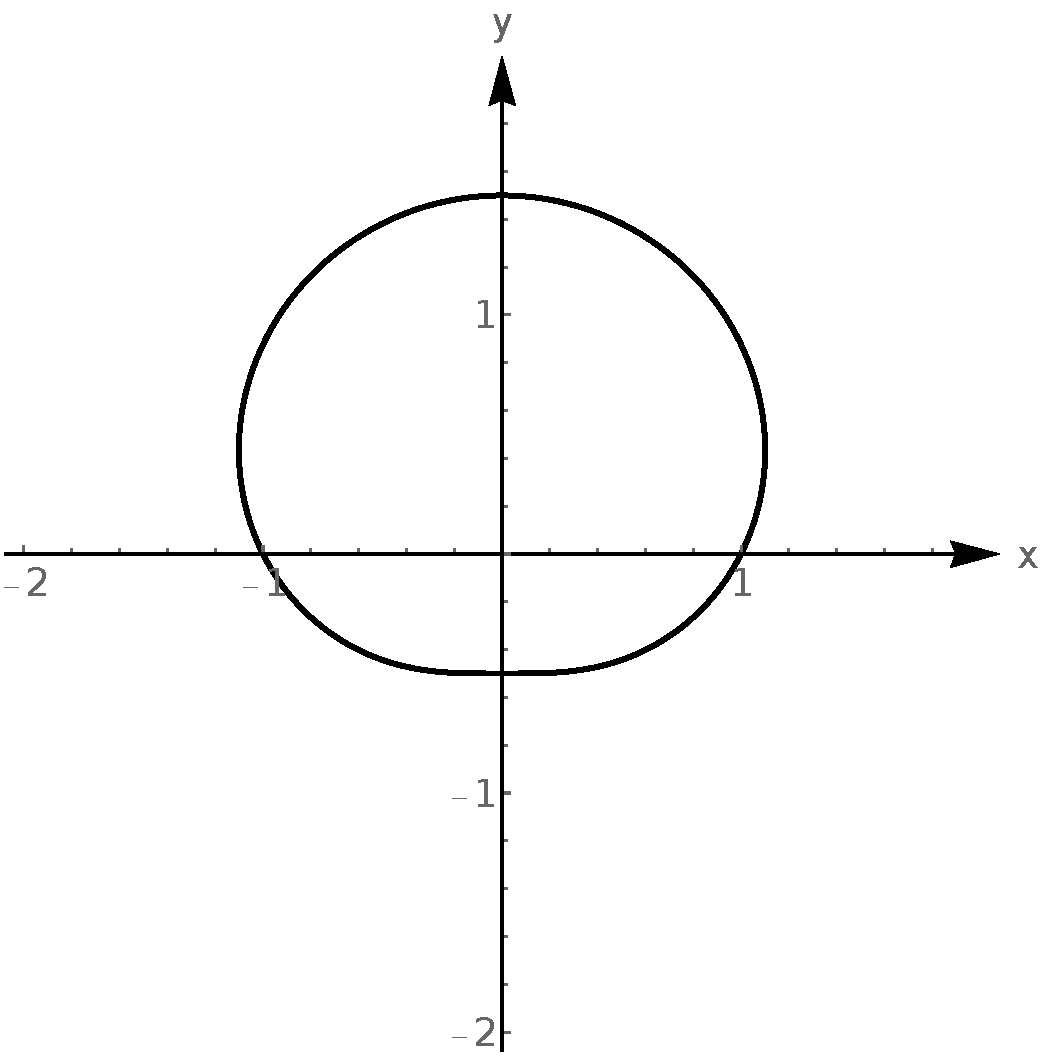
\includegraphics[width=0.33\textwidth]{fig_PGE_1e}}
%(-x,-y)
\hspace*{0.5cm}
\subfigure[]{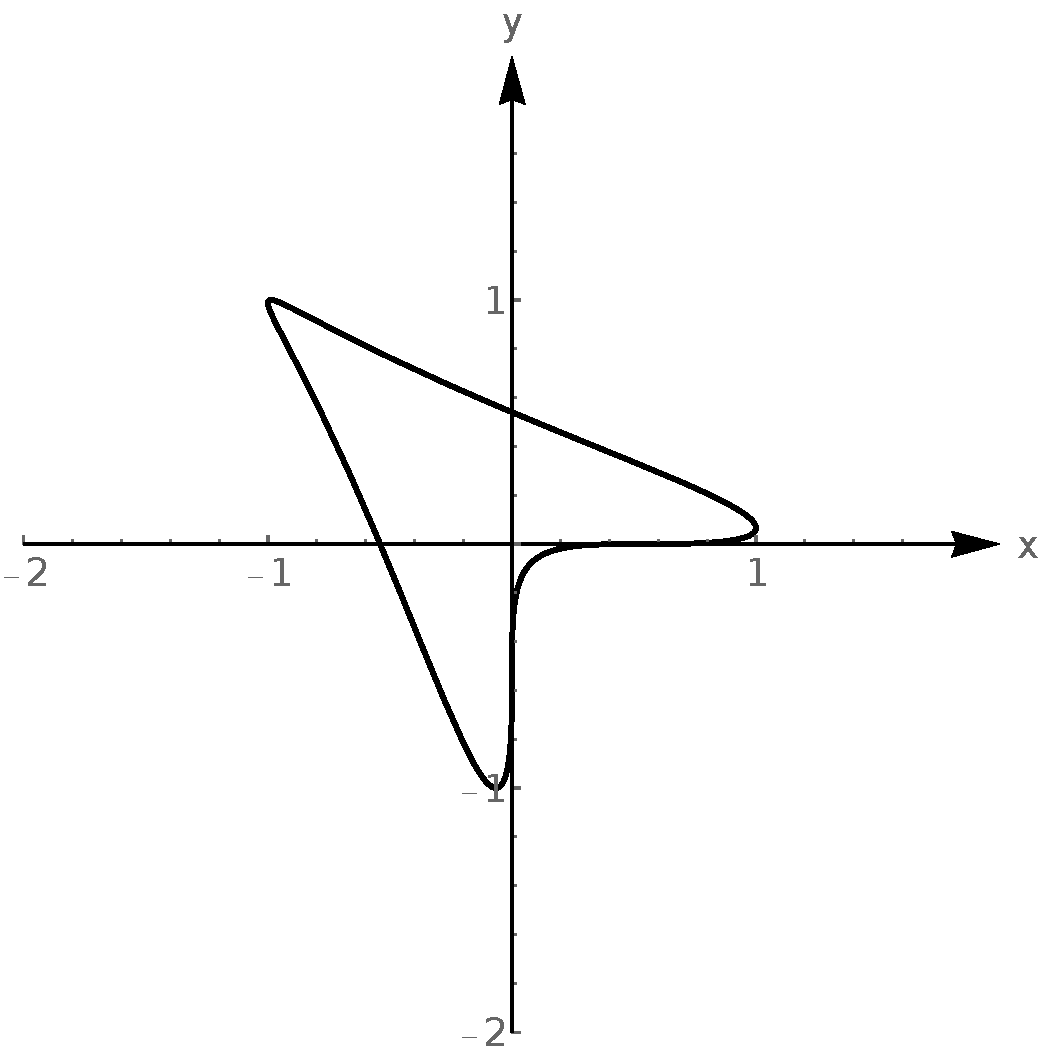
\includegraphics[width=0.33\textwidth]{fig_PGE_1f}}
%(0,x)
}
\caption{\label{fig_test1_1}}

\end{figure}
\end{Exercise}

\begin{Answer}
(1) e;\quad (2) c;\quad (3) f;\quad (4) d;\quad (5) a;\quad (6) b     
\end{Answer}



\begin{Exercise} Determine whether the divergence and rotation of the vector fields in Figure~\ref{fig_test1_2} is positive, negative or zero.
\begin{figure}[H]
\centering
%\raisebox{0.5cm}{
\centerline{
\subfigure[]{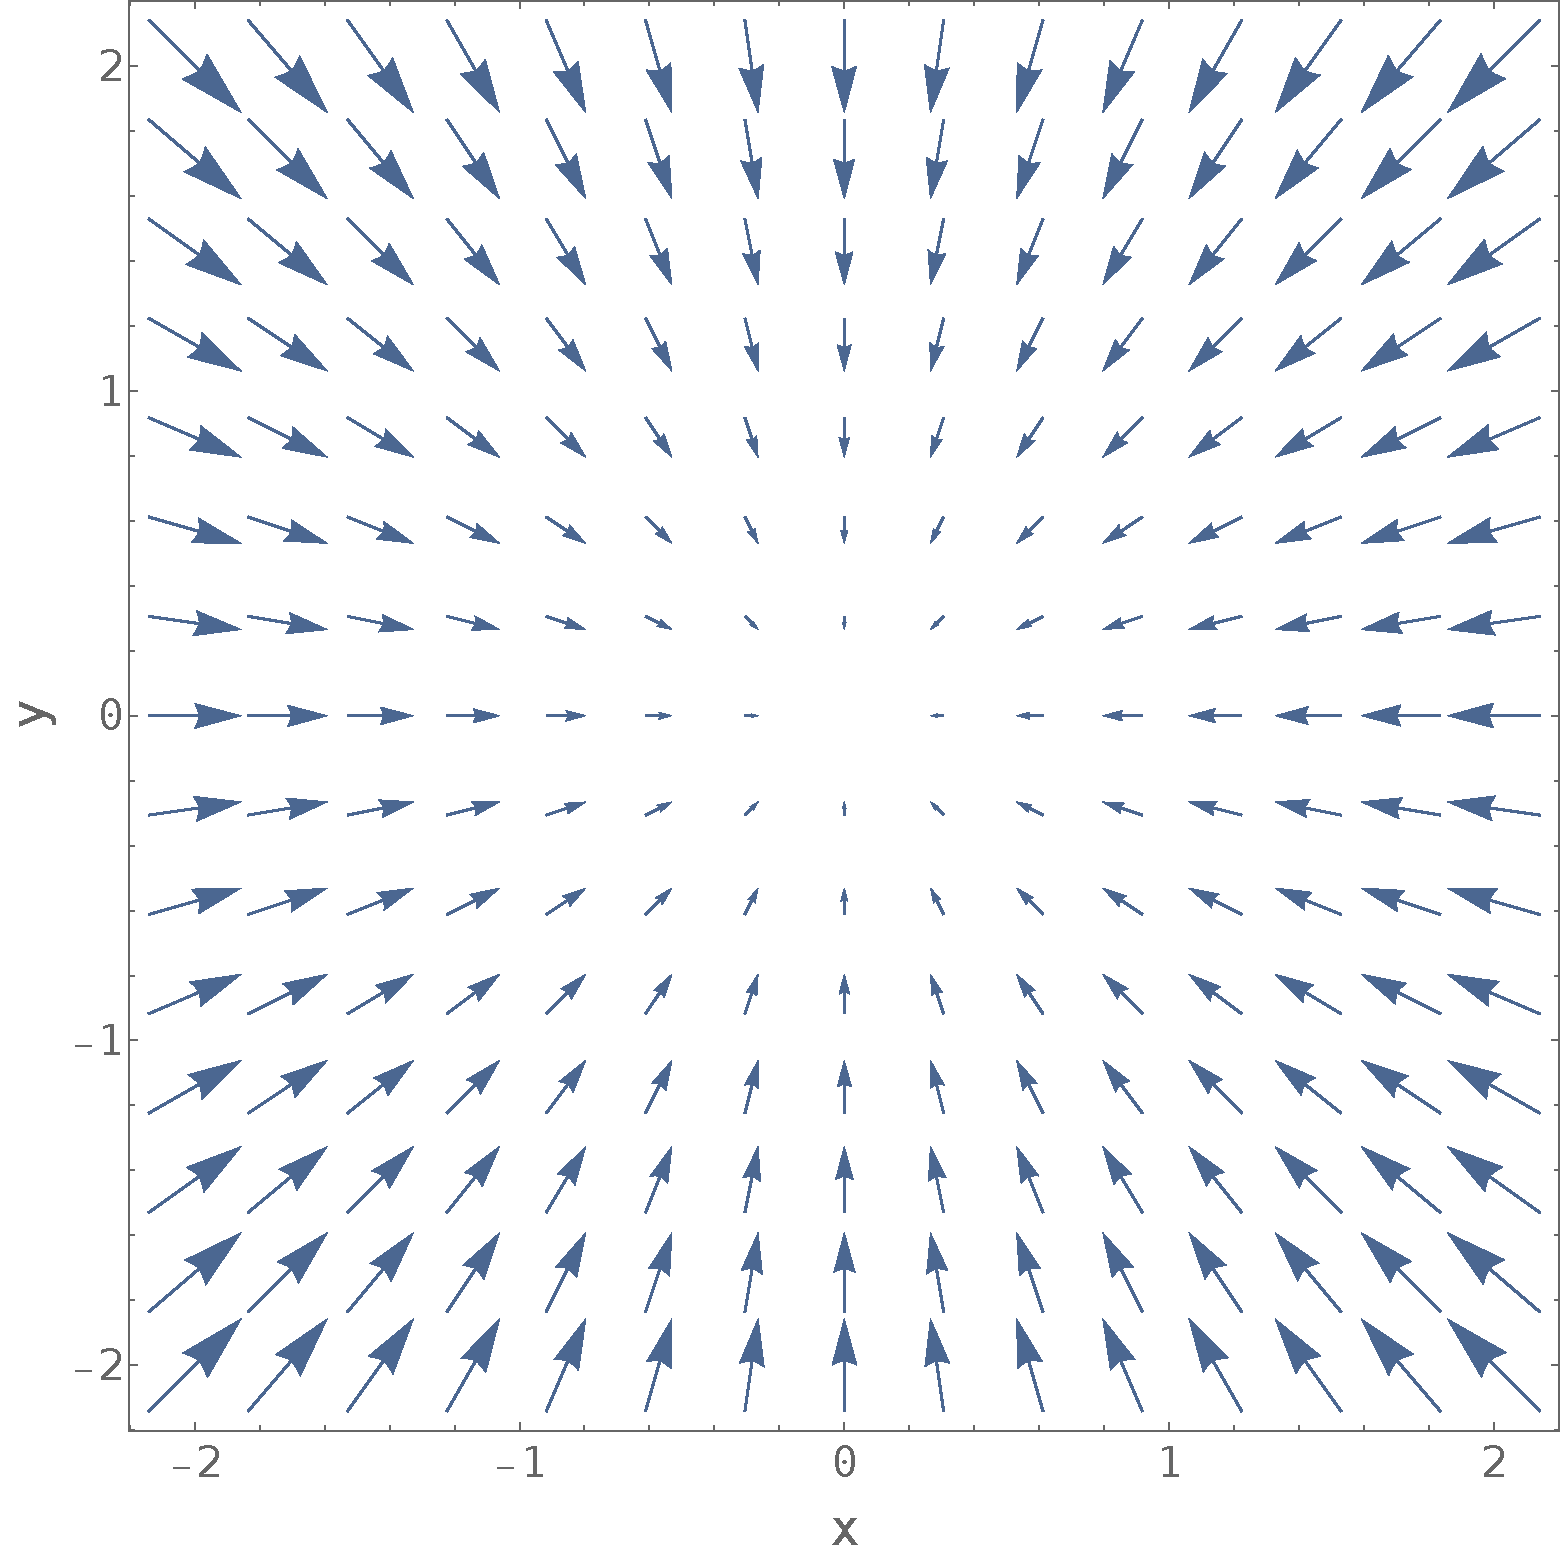
\includegraphics[width=0.48\textwidth]{fig_PGE_2a}}
\subfigure[]{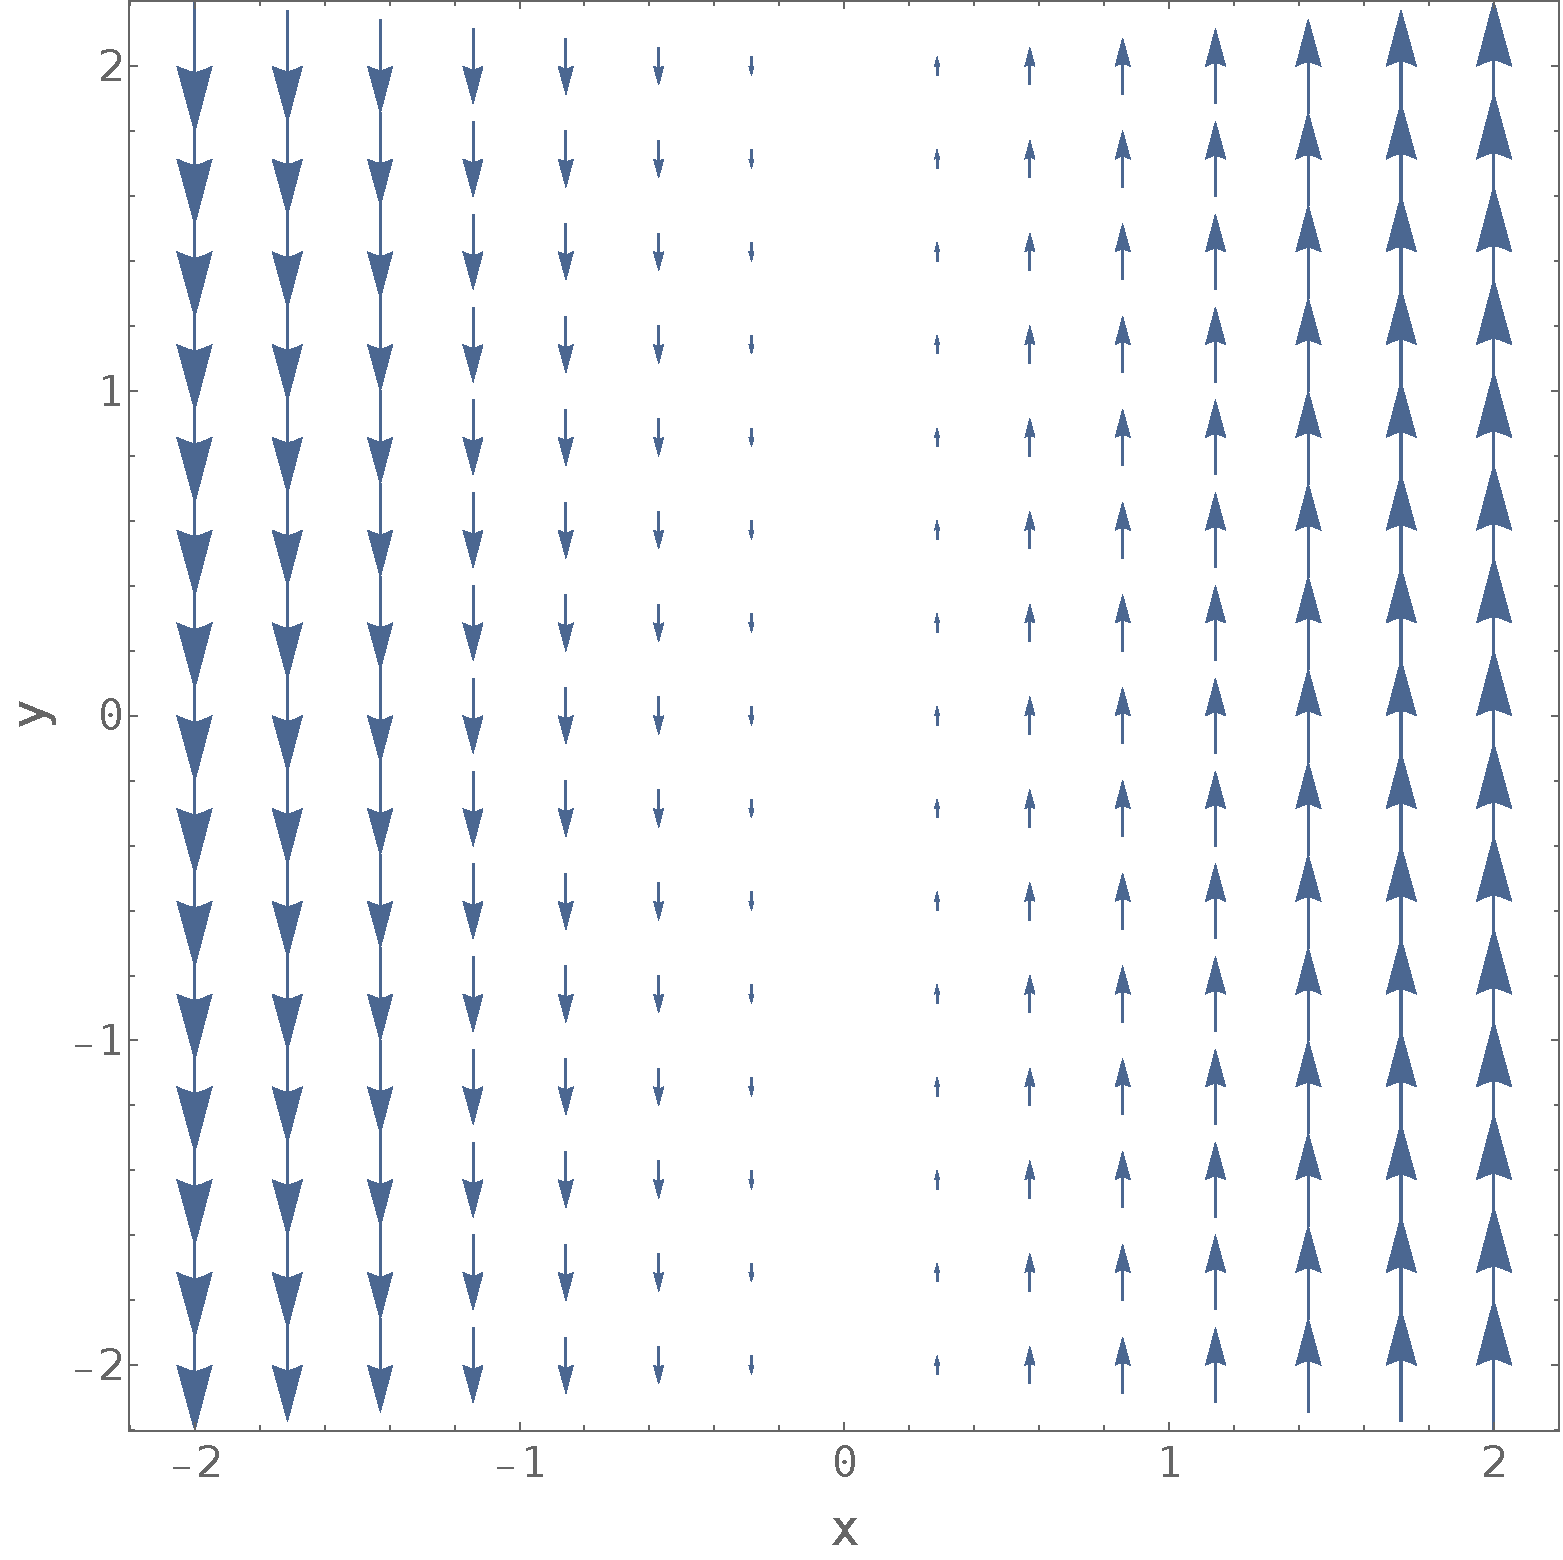
\includegraphics[width=0.48\textwidth]{fig_PGE_2b}}
}
\caption{\label{fig_test1_2}}

\end{figure}
\end{Exercise}

\begin{Answer}
(a) Negative divergence and rotation 0;\quad (b) Divergence 0 and positive rotation.    
\end{Answer}


\begin{Exercise} Consider the curve defined by $y=x^2-1$ and suppose that we want to find the zero points of $x^2-1=0$ using Newtons method.
\Question What will happen if we start this method from the point $x_0=0$? 
\Question Argue whether we best start this method from the point $x_0=0.2$ or $x_0=10$. 
% SMITH 311
\end{Exercise}

\begin{Answer}

\Question The method cannot be performed because there are no intersections with the $x$-axis.
\Question Best to start from $x_0=10$, because the tangent will have a steeper slope. In the case $x_0=0.2$ you will end up far from zero.
    
\end{Answer}



\begin{Exercise} Write down the integral that allows you to calculate the volume of the body of revolution created by rotating the area bounded by the $x$-axis, the $y$-axis and the graph of the function $f(x)=-x^2+2x+3$ around the
\Question $y$-axis  % 0.25
\Question the line $y=-1$. %0.5
\end{Exercise}

\begin{Answer}

\Question $\displaystyle V = 2\pi\int_0^3 x(-x^2+2x+3)\, dx $
\Question $\displaystyle V = \pi\int_0^3 \left[(-x^2+2x+4)^2-1\right] dx $
    
\end{Answer}



\begin{Exercise} Determine the surface area of rotation of the body created by rotating the curve described by $x=t$ and $y=t^3$ around the $x$-axis for $0\leq x\leq1$.
\end{Exercise}

\begin{Answer}
$\displaystyle SA = 2\pi\int_0^1 x^3\sqrt{1+9x^4}\, dx = \dfrac{\pi}{9} \left(\dfrac{10\sqrt{10}}{3}-\dfrac{1}{3}\right)$    
\end{Answer}





\begin{Exercise}If $w=x^2y+z^2$ with $x=\rho\cos(\theta)\sin(\phi)$, $y=\rho\sin(\theta)\sin(\phi)$ and \linebreak $z=\rho\cos(\phi)$, determine then $\frac{\partial w}{\partial \theta}$ and $\frac{\partial w}{\partial \phi}$. 
\end{Exercise}

\begin{Answer}

\Question[] $\displaystyle\frac{\partial w}{\partial \theta} = \frac{\partial w}{\partial x}\frac{\partial x}{\partial \theta} + \frac{\partial w}{\partial y}\frac{\partial y}{\partial \theta} = -2xy\rho\cos(\theta)\sin(\phi) +x^2\rho\cos(\theta)\sin(\phi)$

\Question[] $\displaystyle\frac{\partial w}{\partial \phi} = \frac{\partial w}{\partial x}\frac{\partial x}{\partial \phi} + \frac{\partial w}{\partial y}\frac{\partial y}{\partial \phi} + \frac{\partial w}{\partial z}\frac{\partial z}{\partial \phi}  = 2xy\rho\cos(\theta)\cos(\phi) +x^2\rho\sin(\theta)\sin(\phi) -2z\rho\sin(\phi)$

    
\end{Answer}



\begin{Exercise} Determine the volume located under $2x^2+2y^2+z^2=18$, above $z=0$ and within $x^2+y^2=4$.
\end{Exercise}

\begin{Answer}
$\displaystyle V = \int_0^{2\pi} \int_0^2 \sqrt{18-2r^2}\, r\, dr d\theta = \pi\left(18\sqrt{2} - \dfrac{10\sqrt{10}}{3} \right)$    
\end{Answer}




\begin{Exercise} Swap the integration order of
$$
\int\limits_0^1\int\limits_{0}^{\arccos(y)}f(x,y)\,dx\,dy\,.
$$
\end{Exercise}

\begin{Answer}
$\displaystyle I = \int_0^{\pi/2} \int_0^{\cos(x)} f(x,y)\, dy dx$    
\end{Answer}



\begin{Exercise} A particle moves through a helicoidal orbit given by
$$
\vec{r}(t)=6\cos(\pi\,t)\hat{i}+6\sin(\pi\,t)\hat{j}+2t\hat{k}\,,
$$
with $t\geq0$, towards a spherical tumor cell with cartesian equation given by
$$
x^2+y^2+z^2=100\,.
$$
\Question Determine when the particle arrives at the wall of the tumor cell.
\Question Determine where the particle enters the tumor cell.
\Question Determine the angle at which the particle enters the tumor cell. 
\end{Exercise}

\begin{Answer}

\Question $t=4$
\Question $\vec{r}(4) = (6,0,8)$
\Question $\alpha = \dfrac{\pi}{2} - \arccos\left(\dfrac{-4}{5\sqrt{9\pi^2+1}}\right)$
    
\end{Answer}




\begin{Exercise} The so-called error function is used, among other things, to describe groundwater flow and is given by
\[f(x)=\ds \int\limits_0^x e^{-u^2}\ du\,. \]
However, the integral cannot be calculated analytically and numerical integration is not evident here either. However, the function can be approximated using a Taylor series development. Determine the MacLaurin series development of this function up to fourth order terms. 
\end{Exercise}

\begin{Answer}
    $f(x)=\ds \int\limits_0^x e^{-u^2}\ du = \ds \int\limits_0^{x} \left(1 - u^2 + \dfrac{u^4}{2!} - \dfrac{u^6}{3!} + \ldots \right)\ du = x- \dfrac{x^3}{3.1!} + \dfrac{x^5}{5.2!} -\dfrac{x^7}{7.3!}  + \ldots $
\end{Answer}








%%%%%%%%%%%%%%%%%%%%%%%%%%%
%Examen Wiskunde I/A aug 2019
%%%%%%%%%%%%%%%%%%%%%%%%%%%
\section{Exam August 2019}
\begin{Exercise} For each statement, indicate whether it is True or False. Also, give a brief motivation for your answer. 

\Question Given the function $f:\mathbb{R} \to \mathbb{R}$ with the graph below being the figure.
\begin{center}
\begin{tikzpicture}[scale=1]

        \def\xmin{-1}
        \def\xmax{5}
        \def\ymin{-1}
        \def\ymax{3}
%        \draw[style=help lines, ystep=1, xstep=1] (\xmin,\ymin) grid (\xmax,\ymax);

        \draw (0,0) node[below] {$0$};
				\draw (2,0) node[below] {$2$};
				\draw (4,0) node[below] {$4$};
				\draw (0,2) node[left] {$1$};
				\draw (5,0) node[below] {$x$};
				\draw (0,2.5) node[left] {$y$};
				\draw (2.8,1.5) node[right] {$y=f(x)$};

	
				\draw[->]  (0,0) -- (5,0);
				\draw[->]  (0,0) -- (0,2.5);
				\draw[-]  (2,0) -- (2,0.1);
				\draw[-]  (4,0) -- (4,0.1);
				\draw[-, style=dotted]  (0,2) -- (2,2);

%        \draw plot [domain=0:8,samples=300] (\x,{3-6*cos(\x/2 r)});
			\draw plot [domain=0:2,samples=300] (\x,\x);
			\draw plot [domain=2:4,samples=300] (\x,{4-\x});

    \end{tikzpicture}
\end{center}
Furthermore, the function $g$ is given by $g:\mathbb{R}\to \mathbb{R}: x\mapsto g(x)=x/2$. Then the figure below shows the graph of the product $p$ of these functions \\ $p:\mathbb{R} \to\mathbb{R}: x\mapsto p(x)=f(x) \cdot g(x)$.

\begin{center}
\begin{tikzpicture}[scale=1]

\def\xmin{-1}
\def\xmax{5}
\def\ymin{-1}
\def\ymax{3}
%        \draw[style=help lines, ystep=1, xstep=1] (\xmin,\ymin) grid (\xmax,\ymax);

\draw (0,0) node[below] {$0$};
\draw (2,0) node[below] {$2$};
\draw (4,0) node[below] {$4$};
\draw (0,2) node[left] {$1$};
\draw (5,0) node[below] {$x$};
\draw (0,2.5) node[left] {$y$};


\draw[->]  (0,0) -- (5,0);
\draw[->]  (0,0) -- (0,2.5);
				\draw[-]  (2,0) -- (2,0.1);
\draw[-]  (4,0) -- (4,0.1);
\draw[-, style=dotted]  (0,2) -- (2,2);

%        \draw plot [domain=0:8,samples=300] (\x,{3-6*cos(\x/2 r)});
\draw plot [domain=0:2,samples=300] (\x,{\x^2/2});
\draw plot [domain=2:4,samples=300] (\x,{(4-\x)^2/2});

\end{tikzpicture}
\end{center}
% Fout: neergaande stuk moet gaan volgens een bergparabool

\Question The equation of the function whose graph is a parabola with top in $(3,2)$ and second derivative $-4$ is given by  $f(x)=-2x^2+12x-16$.
%Correct

	
\Question $\arcsin \left(\sin \left(\dfrac{3\pi}{4} \right) \right) = \dfrac{3\pi}{4}$
	%Fout
	
\Question If $f(x)$ and $g(x)$ are polynomial functions, then the rational function has $h(x)=\frac{f(x)}{g(x)}$ a vertical asymptote at the height of all $x$ for which it holds that $g(x)=0$. 
	% Fout: kan een gat zijn
	
\Question The curvature of the intersection of $x^2+y^2+z^2=1$ and $ax+by+cz=0$ is constant and equal to 1.
	% True: Varberg 614
	
		
\Question The tangent to the curve $\vec{r}(t)= (t,2t,3t^2)$ at the origin is perpendicular to the vector $\vec{u}=(2,-1,3)$.

\Question The contour lines of the graph of $f(x,y)=y^2 + (x-2)^2$ are all circles.
	%Fout, bij negatieve C punten.
	
\Question The function $f(x,y,z) = x + y^2 + z^3$ descends the quickest in the point $(0,1,1)$ in the direction of $\hat{\imath} + 2 \hat{\jmath} + 3 \hat{k}$. 
	%FOUT: snelste toename in deze richting.
	
	
\Question Consider a point $P$ on a curve $C$ for which there are two different parametrisations available, being\ $\vec{r}_1(t)$ and $\vec{r}_2(t)$. Then the tangent vector according to $\vec{r}_1(t)$ in $P$ the same as these according to $\vec{r}_2(t)$.
	% Uit:multivar_meerkeuze2 p6
	% Fout: zie voorbeeld 18.2 en aanvulling les
	
	
\Question Consider the vector field $\vec{F}(x,y,z) = (x+\sin(y), y - \sin(z), z)$. The divergence of this vector field is equal to $(1,1,1)$.
	%FOUT: div F = 3
\end{Exercise}


\begin{Answer}
\Question False. The part between $x=2$ and $x=4$ describes part of a parabola that opens downwards and therefore not a parabola that opens upwards.
\Question True. From the first derivative, the top of the parabola easily follows and the second derivative confirms that this is the top of a parabola that opens downwards.

	
\Question False. $\dfrac{3\pi}{4}\notin \mbox{im } \arcsin = \left[-\dfrac{\pi}{2},\dfrac{\pi}{2}\right]$
	
\Question False. If $f(x)$ and $g(x)$ are simultaneously 0, then a perforation point and not a VA occurs.
	
\Question True. The cross section is a circle centered at the origin and radius 1.
		
\Question True. The scalar product of $\vec{r}'(0)$ and $\vec{u}$ equals 0.

\Question False. For negative values of $C$ we get nothing, because $y^2+(x-2)^2\geq 0$.
	
\Question False. It's the direction of the fastest increase.
	
\Question False. Consider e.g. the circle with equation $x^2+y^2=4$ and parametrisations $\vec{r}_1(t)=(2\cos(t),2\sin(t))$ and $\vec{r}_2(t)=\left(t,\pm\dfrac{t}{\sqrt{4-t^2}}\right)$. Then it is clear from the first derivations that the tangent vectors are different.

\Question False. The divergence is $1+1+1 = 3$.
\end{Answer}


\begin{Exercise} For each graph in Figure~\ref{grafs} determine the appropriate equation.
\begin{multicols}{3}
\begin{enumerate}
\item[]
\item[]
\item[]
\item[(1)] $y=\arccos(2\cos(x))$
\item[(2)] $y=\arccos(2\cos(|x|))$
\item[(3)] $y=\arccos(2|\cos(x)|)$
\item[(4)] $y=\cos(2\arccos(x))$
\item[(5)] $y=\cos(2\arccos(|x|))$
\item[(6)] $y=\cos(2|\arccos(x)|)$ 
\end{enumerate}
\EndCurrentQuestion
\end{multicols}


\begin{figure}[H]
%\centering
\centerline{
\subfigure[]{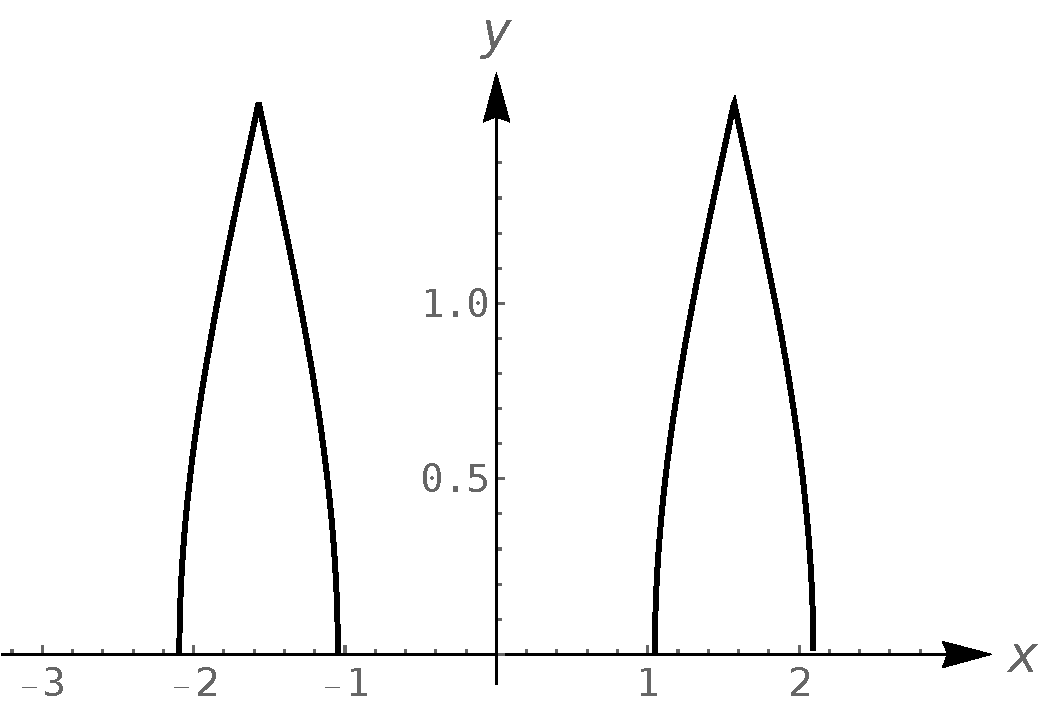
\includegraphics[width=0.45\textwidth]{grafs_ing_1}}
%%(-x,-y)
\hspace*{0.5cm}
\subfigure[]{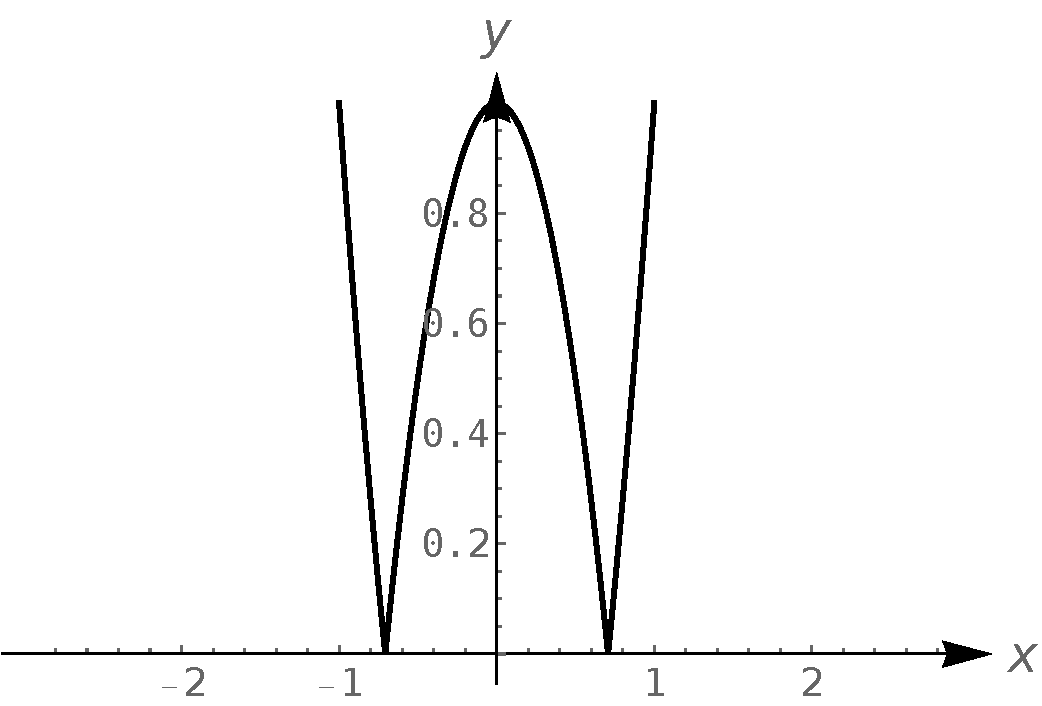
\includegraphics[width=0.45\textwidth]{grafs_ing_2}}
}
\centerline{
\subfigure[]{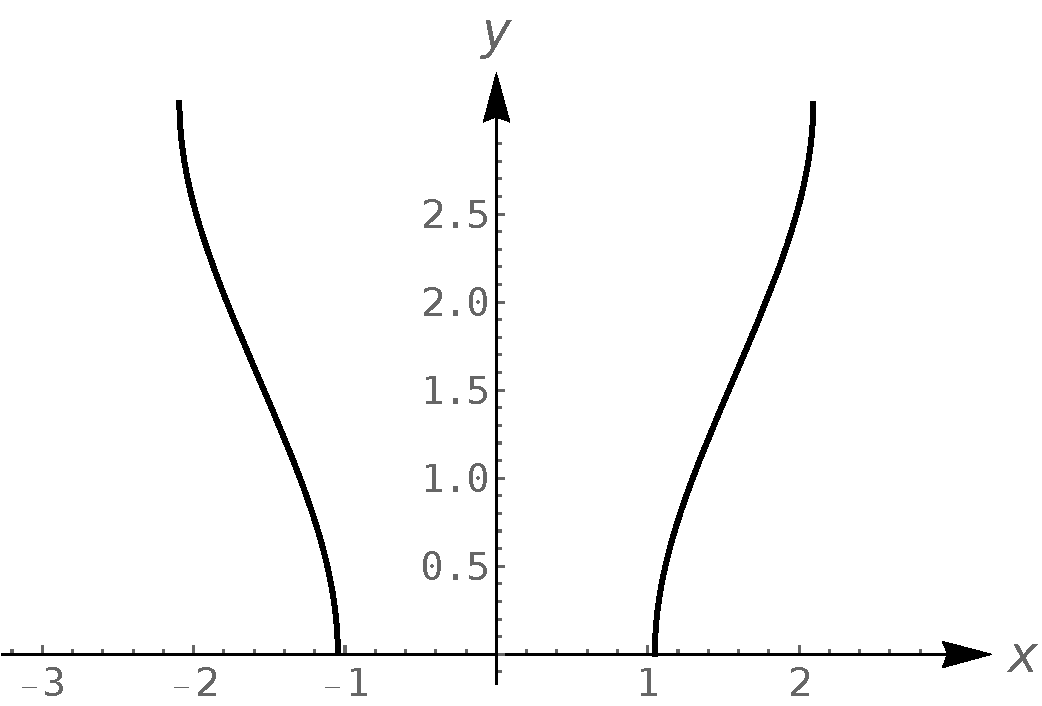
\includegraphics[width=0.45\textwidth]{grafs_ing_3}}
\hspace*{0.5cm}
\subfigure[]{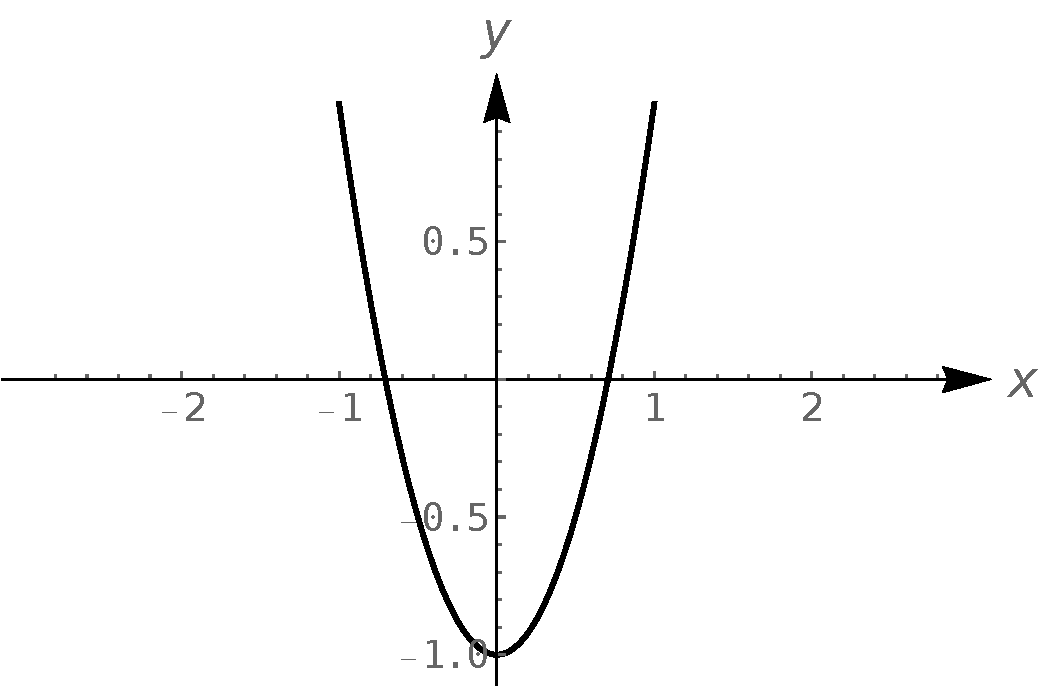
\includegraphics[width=0.45\textwidth]{grafs_ing_4}}
}
\caption{\label{grafs}}
\end{figure}
\end{Exercise}

\begin{Answer}
(1) c;\quad (2) c;\quad (3) a;\quad (4) d;\quad (5) d;\quad (6) b    
\end{Answer}


\begin{Exercise}  Consider the trapezoidal method over the interval $[a,b]$, which we divide into $n$ subintervals for calculating 
$$
\int\limits_a^bf(x)dx\,.
$$
For the absolute total error $E$ on this method, i.e., the total deviation between the determined integral and its numerical approximation, it is true that
$$
E\leq\dfrac{\max|f''(\xi)|(b-a)^3}{12n^2}\,,
$$
with $\xi\in[a,b]$.
\Question For which function family does this method work flawlessly?
\Question Give two examples of functions for which we are assured that $0<E\leq b^3/(12n^2)$ if we are working over $[0,b]$.
\end{Exercise}

\begin{Answer}
\Question Constant and linear functions.
\Question $f(x)=\sin(x)$ en $f(x)=\cos(x)$
\end{Answer}


\begin{Exercise}  Calculate the limit below.
\[ \lim\limits_{x \to 2} \left( \dfrac{1}{x-2} - \dfrac{1}{|x-2|} \right) \]
% x>2: 0; x<2: -\infty
\end{Exercise}

\begin{Answer}
 $\lim\limits_{x \to 2} \left( \dfrac{1}{x-2} - \dfrac{1}{|x-2|} \right)$ does not exist, but $\lim\limits_{x \stackrel{>}{\to} 2} \left( \dfrac{1}{x-2} - \dfrac{1}{|x-2|} \right)=0$ and  $\lim\limits_{x \stackrel{<} {\to}2} \left( \dfrac{1}{x-2} - \dfrac{1}{|x-2|} \right)=-\infty$
\end{Answer}

\begin{Exercise} For each of the statements below, compose the integral that allows you to compute the demand. Write the integrand as simply as possible.
\Question The surface of the area within $r=-4\cos(\theta)$ and $r=-4\sin(\theta)$; %Ings

\Question the distance travelled by a particle that moves between $t=0$ en $t=1$ along the curve $C$ parameterized by $\vec{r}(t)=\left(e^t\sin(t),e^t\cos(t)\right)$;
%Ings

\Question the work performed by a particle moving along the curve $C$ parameterized by $\vec{r}(t)=\left(1+t^2,1+\sin(\pi t)\right)$ going from $t =0$ to $t=1$ and thereby subject to the field $\vec{F}=\left(\dfrac{1}{y},1- \dfrac{x}{y^2}\right)$.
\end{Exercise}

\begin{Answer}
\Question $\displaystyle O = \dfrac{1}{2} \int_{\pi}^{5\pi/4} 16\sin^2(\theta)\, d\theta + \dfrac{1}{2} \int_{5\pi/4}^{3\pi/2} 16\cos^2(\theta)\, d\theta$    
\Question $\displaystyle s=\sqrt{2}\int_0^1 e^t\, dt$
\Question $A = \displaystyle \int_0^1 \left( \dfrac{2t}{1+\sin(t\pi)} , \pi\cos(t\pi) - \dfrac{\pi(1+t^2)\cos(t\pi)}{(1+\sin(t\pi))^2} \right) dt$
\end{Answer}


\begin{Exercise} A water reservoir has a parabolic shape with the equation of the underlying parabola being $y=ax^2$. The maximum depth of water in this reservoir is 8 m and when the reservoir is filled to a height of 5 m, the water surface has a diameter of 20 m. What is the maximum volume of water that this reservoir can hold?
\end{Exercise}

\begin{Answer}
The maximum water volume is $640\pi$ m$^3$.
\end{Answer}


\begin{Exercise} Consider the curve
$$
\arctan(x+y)=x^2+\dfrac{\pi}{4}\,,
$$
where we assume that $y=f(x)$. 
\Question Determine the equation of the tangent to the given curve at the point with $x=0$. 
\Question Determine the concavity of the curve at this point.
\end{Exercise}

\begin{Answer}
\Question $y=-x+1$
\Question $y''(0,1)=4$
\end{Answer}


\begin{Exercise}  Examine the convergence of
$$
\int\limits_{0}^{+\infty}e^{-x}\sin(x)\, dx.
$$
%Berekenen, oefening uit cursus: oef 8(b) Hoofdstuk 12
\end{Exercise}

\begin{Answer}
Convergent.    
\end{Answer}


\begin{Exercise} Determine the Maclaurin series expansion of the function 
$$
f(x)=2x^3\,\cos\left(4x^5\right)\,.
$$
\end{Exercise}

\begin{Answer}
$\displaystyle f(x)=2x^3\,\cos\left(4x^5\right)=2\sum_{n=0}^{+\infty} \dfrac{(-1)^n\, 4^{2n}\, x^{10n+3}}{(2n)!}$    
\end{Answer}


\begin{Exercise} If $W(s,t) = f(u(s), v(s,t))$. 
\Question  Determine $\frac{\partial W}{\partial s}$ and $\frac{\partial W}{\partial t}$.	
\Question Assume that $u'(1) = 1$, $\frac{\partial v}{\partial s}(1,3) = 1$, $\frac{\partial v}{\partial t}(1,3) = 4$, $u(1)=0$, $v(1,3)=4$, $f_u(0,4)=1$ and $f_v(0,4)=-2$. Determine than $\frac{\partial W}{\partial s}(1,3)$.
\end{Exercise}

\begin{Answer}
\Question $\dfrac{\partial W}{\partial s} = \dfrac{\partial f}{\partial u}\dfrac{du}{ds} + \dfrac{\partial f}{\partial v}\dfrac{\partial v}{\partial s}$ \qquad and\qquad $\dfrac{\partial W}{\partial t} = \dfrac{\partial f}{\partial v}\dfrac{\partial v}{\partial t}$
\Question $\dfrac{\partial W}{\partial s}(1,3)=-1$    
\end{Answer}


\begin{Exercise} Calculate
\[
\int\limits_0^{\sqrt{3}}\int\limits_{\frac{y}{\sqrt{3}}}^{\sqrt{4-y^2}}e^{-x^2-y^2}\,dx\,dy\,.
\]
\end{Exercise}

\begin{Answer}
 $\int\limits_0^{\sqrt{3}}\int\limits_{\frac{y}{\sqrt{3}}}^{\sqrt{4-y^2}}e^{-x^2-y^2}\,dx\,dy = \dfrac{\pi}{6}\left(1-e^{-4}\right)$   
\end{Answer}


\begin{Exercise} Calculate the volume of the body bounded by the cylinders \\ $x^2 + y^2 -y = 0$, $x^2 + y^2 -2y = 0$, $z=2+x$ and the $xy$-plane. 
\end{Exercise}

\begin{Answer}
$\displaystyle V=\int_0^{\pi}\int_{\sin(\theta)}^{2\sin(\theta)}\int_0^{2+r\cos(\theta)} r\, dz dr d\theta = \dfrac{3\pi}{2}$    
\end{Answer}


%%%%%%%%%%%%%%%%%%%%%%%%%%%
%Examen Calculus jan 2020
%%%%%%%%%%%%%%%%%%%%%%%%%%%
\section{Exam January 2020}
\begin{Exercise} For each statement, indicate whether it is True or False. Also, give a brief motivation for your answer. 

\Question The tangents to the graphs of the functions $f(x)=x^3$ and $g(x)=\frac{1}{3x}$ are in every point $x \neq 0$ perpendicular to each other.
	%Juist
	%%%%%%%%%%%%%%%
\Question  The function
	$$
	F(x)=\displaystyle\int\limits_a^xf(u)\ du
	$$
	is convex  where $f(x)$ inclines and concave where $f(x)$ declines. 
	% Juist
\Question  The MacLaurin series expansion of $f(x)=x^4e^{-3x^2}$ is given by
$$
\sum\limits_{n = 0}^{+\infty} {\frac{{{{\left( { - 3} \right)}^n}{x^{2n + 4}}}}{{n!}}}\,.$$
% Juist
    %%%%%%%%%%%%%%%
	
\Question The contour lines of the function $f(x,y)=\arcsin\left(\sqrt{x^2+y^2}\right)$ are not all circles. 
	% Juist, (0,0) geeft een punt

\Question  The calculation of $\lim\limits_{(x,y)\to(0,0)} f(x,y)$, where
	$$
	f(x,y)=\left\{\begin{array}{rcl}
	\dfrac{xy^2}{x^2+y^4},& \text{ als} &(x,y)\neq(0,0)\,,\\[0.2cm]
	0,& \text{ als}&(x,y)=(0,0)\,,
	\end{array}\right.
	$$
	along $y=x$ and $x=y^2$ allows us to conclude that $f$ is not continuous in $(0,0)$. 
	% Juist
	
\Question A cylindrical tank made of steel has a height of 10m and a diameter of 4m. The steel jacket of the tank expands and contracts under the influence of temperature changes. The tank volume is more sensitive to changes in height than to changes in diameter. 
	% Fout (via differentiaal)
\end{Exercise}


\begin{Answer}
\Question True. The product of the corresponding ricos (first derivatives) is always $-1$.
\Question True. Use that $F'(x)=f(x)$ and $F''(x)=f'(x)$.
\Question True. Transform the MacLaurin series developement of $e^x$.
\Question True. If $C=0$ we have a point.
\Question True. The limit along $y=x$ is 0 and the limit along $x=y^2$ is $1/2$.
\Question False. $dV = 4\pi\, dH + 20\pi\, dD$ and $20\pi>4\pi$.
 
\end{Answer}


\begin{Exercise}Consider the function 
\[ f(x)= \left\{\begin{array}{rcl} 
2x^2+x^2\sin \left( \dfrac{1}{x}\right), & \text{ als} & x \neq0, \\
0, & \text{ als} & x = 0. 
\end{array}  \right.   \]
Discuss the continuity and derivability of the function. $f$ in $[0, +\infty[$. 
\end{Exercise}

\begin{Answer}
The function $f$ is continuous everywhere in $[0, +\infty[$. The function $f$ is derivable if $x\neq 0$ and not derivable if $x=0$.    
\end{Answer}



\begin{Exercise} Figure~\ref{fig_test2_1} shows the graphs of four functions, while Figure~\ref{fig_test2_2} shows the graphs of some of the derived functions. For each of the functions in Figure, fill in the table below~\ref{fig_test2_1} with the letter(s) of the graph(s) of the corresponding derivative function(s).

\renewcommand{\arraystretch}{1.25}
\begin{tabular}{l|c|l|c}
Graph function&Graph derivative &Graph function&Graph derivative\\
&function&& function\\\hline
a&&c&\\[0.2cm]\hline
b&&d&\\
\end{tabular}
\renewcommand{\arraystretch}{1.25}

%
% 	\begin{enumerate}
% 		\begin{multicols}{2}
% 			\item $f(x)=\ln\left(\dfrac{1}{x}\right)$
% 			\item $f(x)=\ln\left(\dfrac{1}{|x|}\right)$
% 			\item $f(x)=\ln\left(\dfrac{-1}{x}\right)$
% 			\item $f(x)=\left|\ln\left(\dfrac{1}{x}\right)\right|$
% 			\item $f(x)=\left(\ln\left(\dfrac{1}{x}\right)\right)^{-1}$
% 		\end{multicols}
% 	\end{enumerate}
 	
\begin{figure}[H]
\centering
%\raisebox{0.5cm}{
\centerline{
\subfigure[]{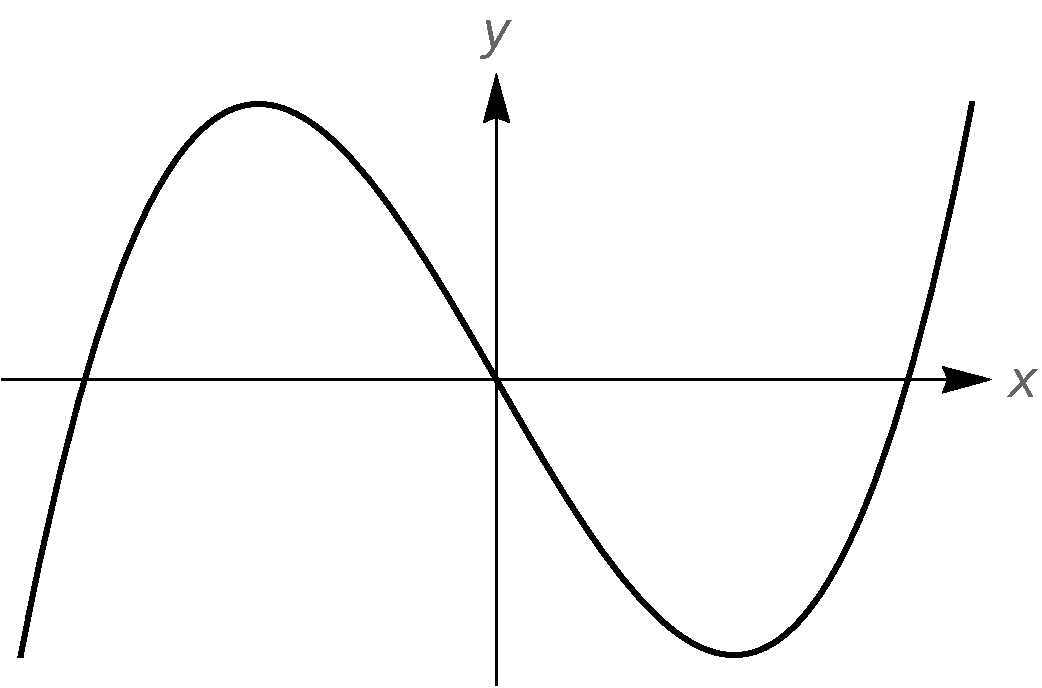
\includegraphics[width=0.33\textwidth]{fig_test2_1a}}
\hspace*{1cm}
\subfigure[]{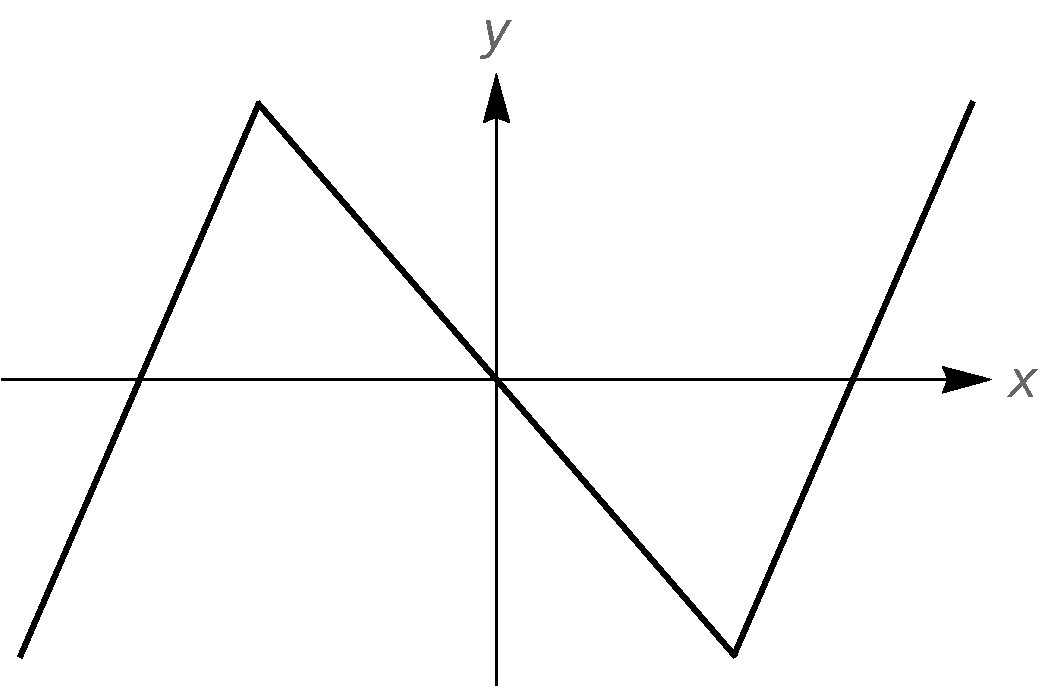
\includegraphics[width=0.33\textwidth]{fig_test2_1b}}
}
\centerline{
\subfigure[]{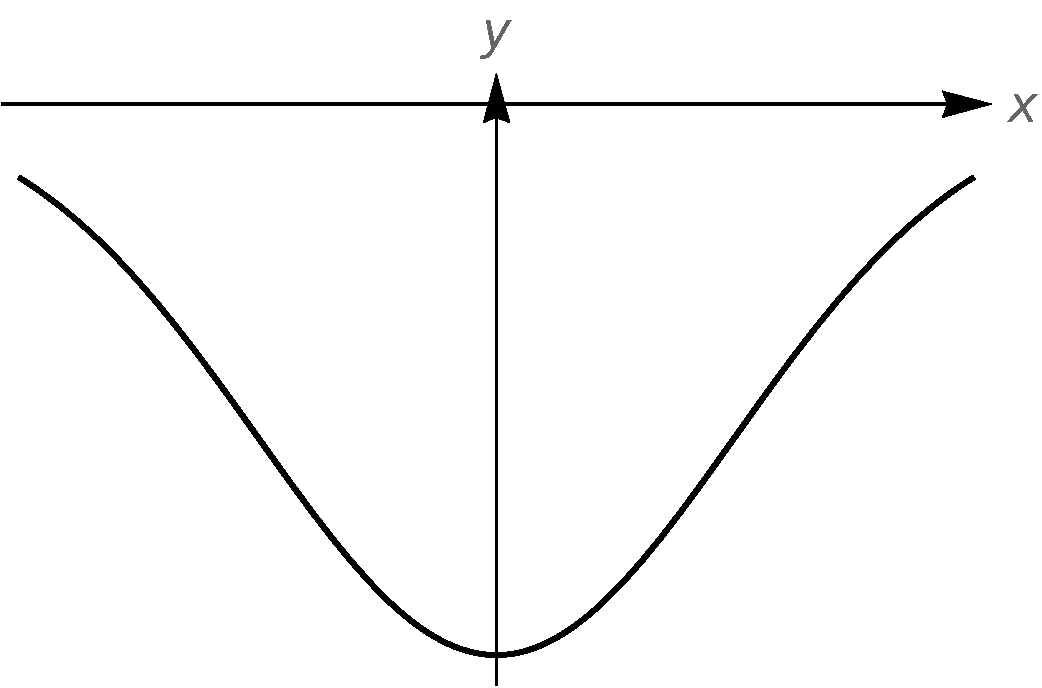
\includegraphics[width=0.33\textwidth]{fig_test2_1c}}
\hspace*{1cm}
\subfigure[]{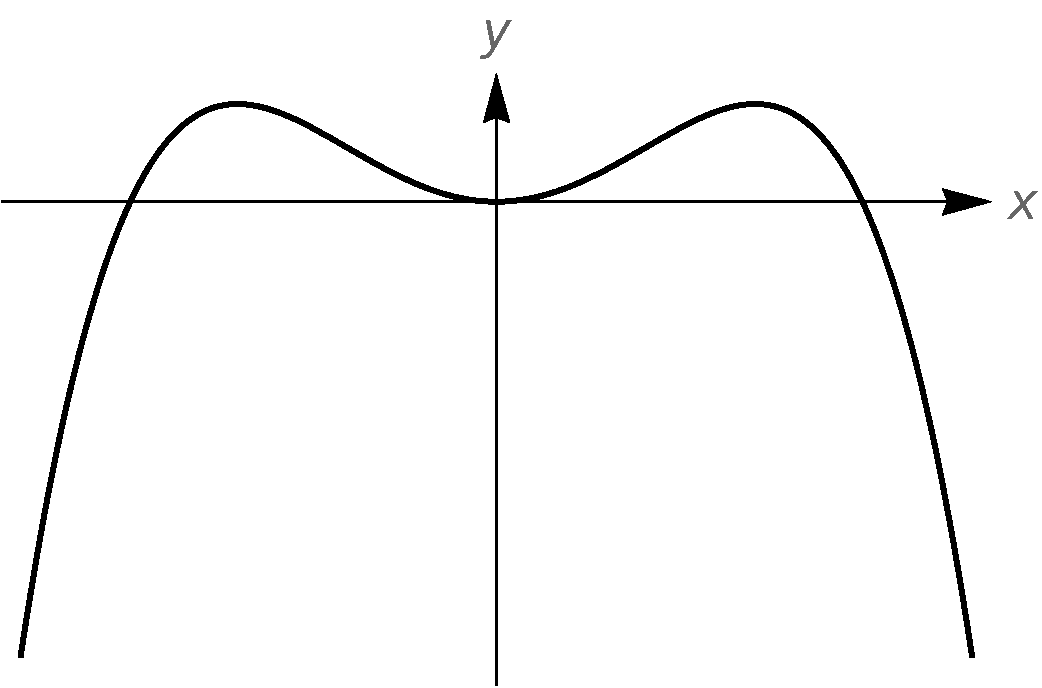
\includegraphics[width=0.33\textwidth]{fig_test2_1d}}
}
\caption{\label{fig_test2_1}}
\end{figure}


\begin{figure}[H]
\centering
%\raisebox{0.5cm}{
\centerline{
\subfigure[]{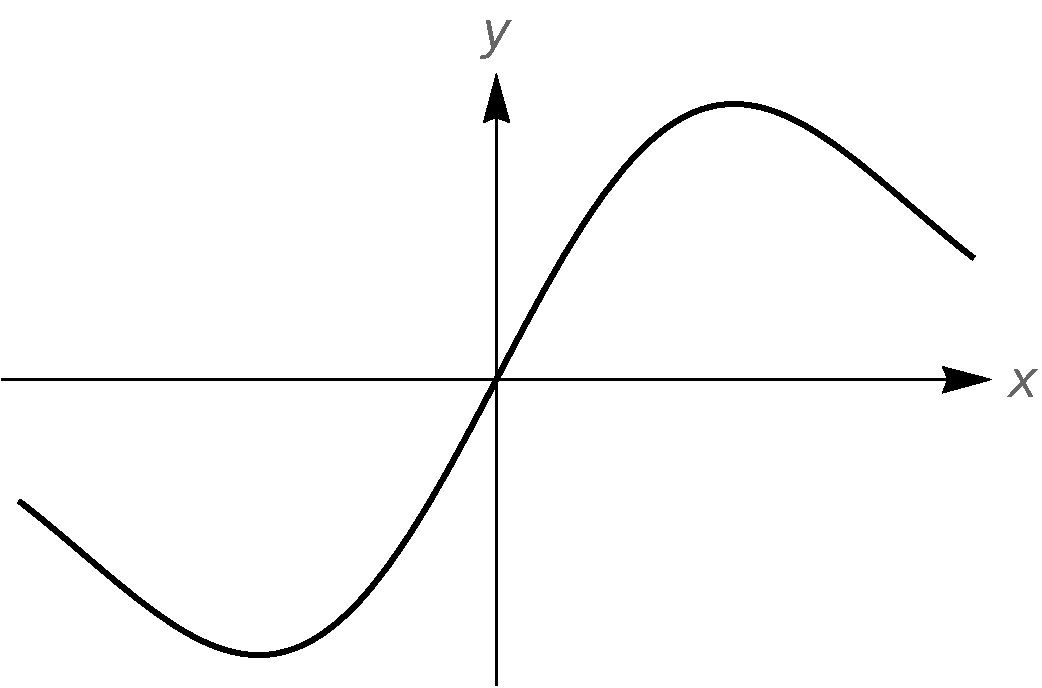
\includegraphics[width=0.33\textwidth]{fig_test2_1copl}}
\subfigure[]{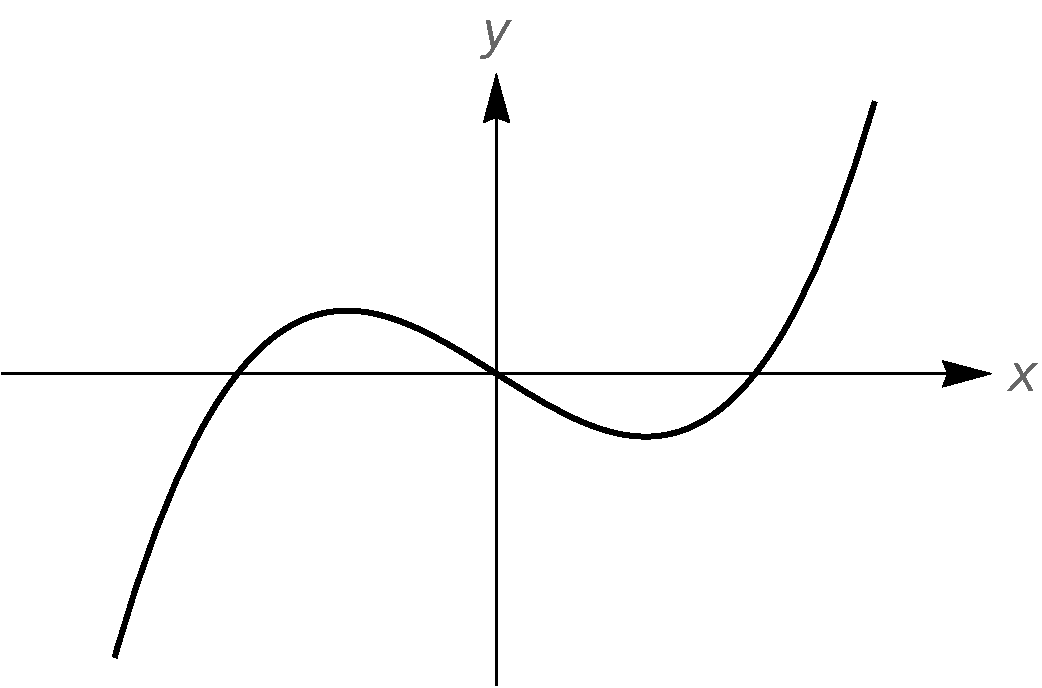
\includegraphics[width=0.33\textwidth]{fig_test2_afleider}}
\subfigure[]{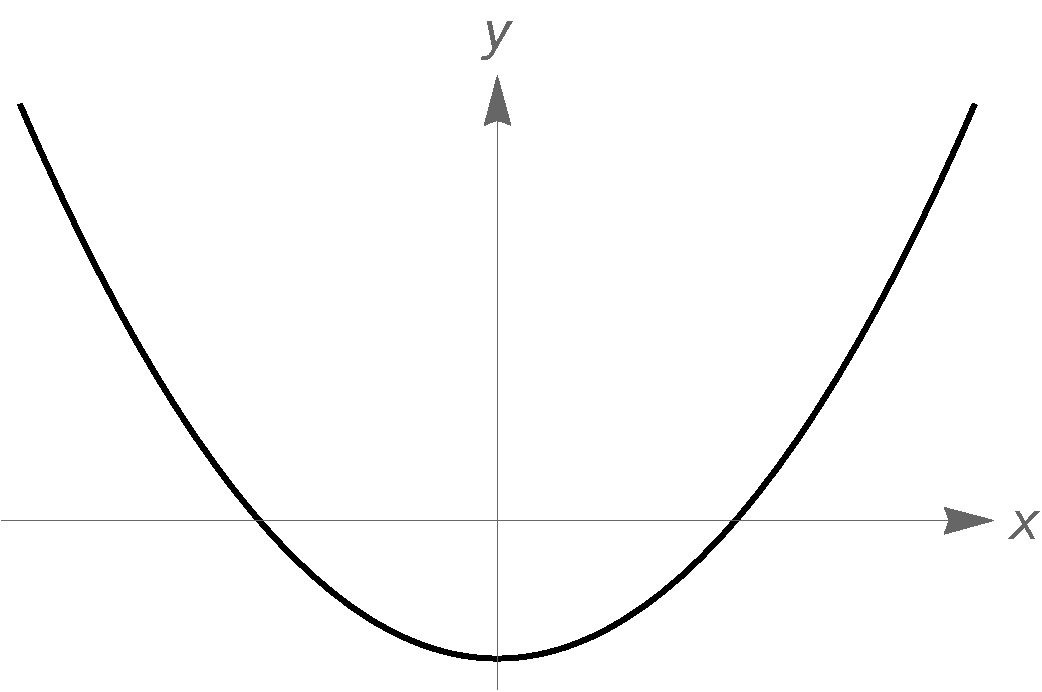
\includegraphics[width=0.33\textwidth]{fig_test2_1aopl}}
}
\centerline{
\subfigure[]{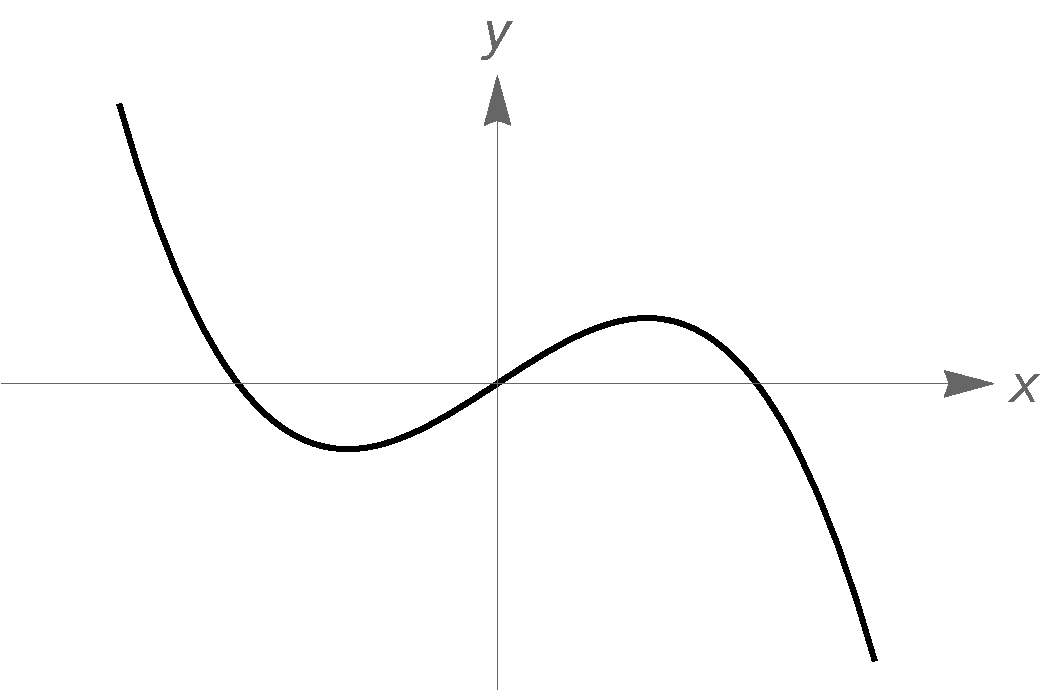
\includegraphics[width=0.33\textwidth]{fig_test2_1dopl}}
\subfigure[]{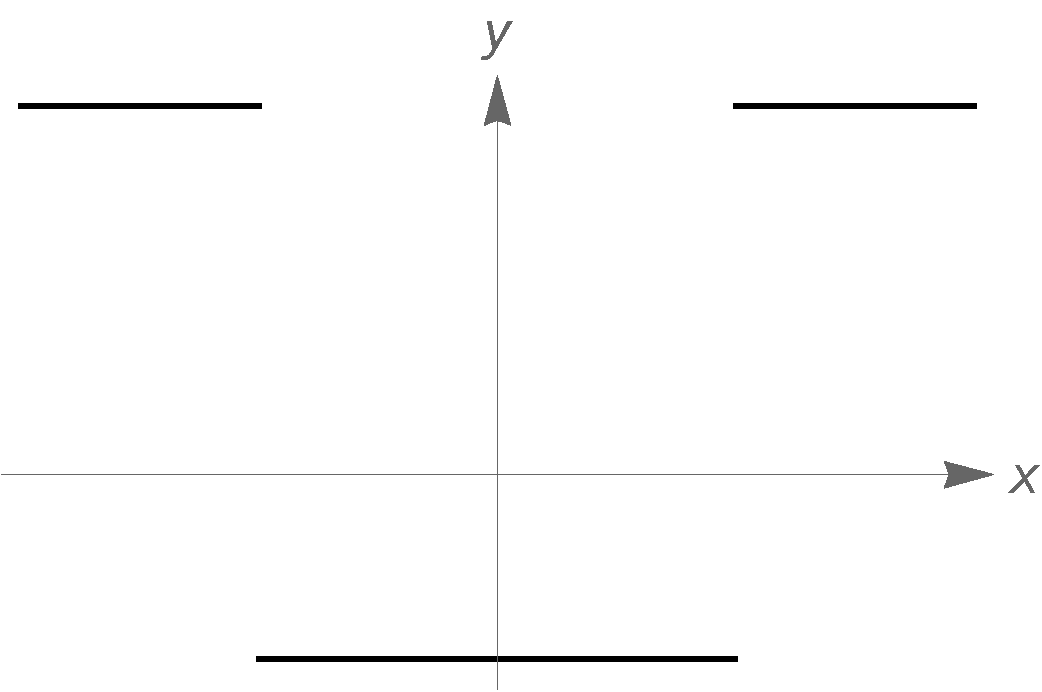
\includegraphics[width=0.33\textwidth]{fig_test2_1bopl}}
}
\caption{\label{fig_test2_2}}
\end{figure}
\end{Exercise}

\begin{Answer}
\renewcommand{\arraystretch}{1.25}
\begin{tabular}{l|c|l|c}
Graph function&Graph derivative &Graph function&Graph derivative\\
&function&& function\\\hline
a&c&c&a\\[0.2cm]\hline
b&e&d&d\\
\end{tabular}
\renewcommand{\arraystretch}{1.25}    
\end{Answer}


\begin{Exercise} Calculate
$$
\displaystyle\int\limits_0^{\frac{\pi}{4}}\dfrac{x\sin(x)}{\cos^3(x)}\,dx\,.
$$
\end{Exercise}

\begin{Answer}
$\displaystyle\int\limits_0^{\frac{\pi}{4}}\dfrac{x\sin(x)}{\cos^3(x)}\,dx = \dfrac{\pi}{4}-\dfrac{1}{2}$    
\end{Answer}



\begin{Exercise} Consider the curve 
\[ x=\sin(\theta), \quad y = \sin(\theta)\cos(\theta)\,, \]
graphically represented in Figure~\ref{lemmiscaat}. 
\Question Determine the value(s) of the parameter $\theta$ for which the curve has a horizontal tangent. Also determine the corresponding points in the $xy$-plane. 
\Question Compose the integral to determine the volume of the body of revolution created by the rotation of this curve about the $y$-axis. 
\Question Compose the integral to determine the volume of the body of revolution created by the rotation of this curve about the $x$-axis. 

\begin{figure}[H]
\centering
%\raisebox{0.5cm}{
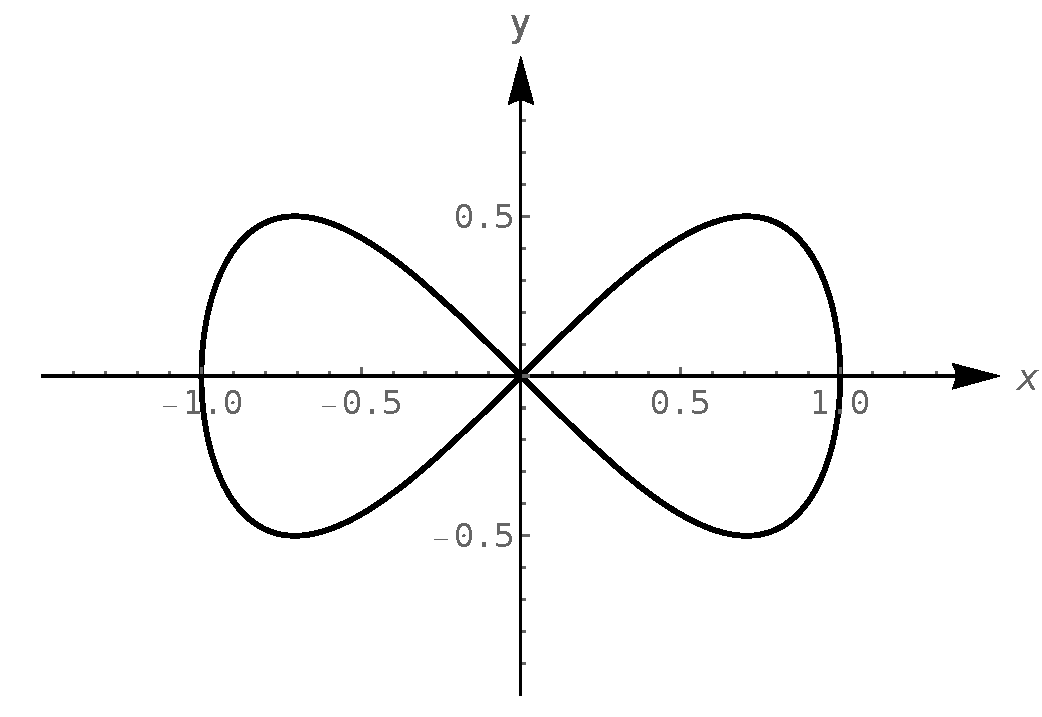
\includegraphics[width=0.75\textwidth]{lemmiscaat}

\caption{\label{lemmiscaat}}
\end{figure}
\end{Exercise}

\begin{Answer}

\Question Horizontal tangent for $\theta = \dfrac{\pi}{4}, \dfrac{3\pi}{4}, \dfrac{5\pi}{4}, \dfrac{7\pi}{4}$. The corresponding points in the $xy$-plane are $\left(\dfrac{\sqrt{2}}{2},\dfrac{1}{2}\right), \left(\dfrac{\sqrt{2}}{2},-\dfrac{1}{2}\right), \left(-\dfrac{\sqrt{2}}{2},\dfrac{1}{2}\right), \left(-\dfrac{\sqrt{2}}{2},-\dfrac{1}{2}\right)$.
\Question $\displaystyle V = 4\pi\int_0^{\pi/2} \sin^2(\theta)\cos^2(\theta)\,d\theta$
\Question $\displaystyle V = 2\pi\int_0^{\pi/2} \sin^2(\theta)\cos^3(\theta)\,d\theta$
    
\end{Answer}


\begin{Exercise} Determine the area of the region enclosed by the curves $y=\sqrt{x}$, $y=-\dfrac{x}{2}+1$, $x=1$ and $x=4$.
%(\url{https://www.math.upenn.edu/~rimmer/math103/exams/103exam3f13.pdf}) (vraag 6) 
\end{Exercise}

\begin{Answer}
$A = \dfrac{65}{12} $    
\end{Answer}



\begin{Exercise} The cat Kamiel moves according to $\vec{r}(t)=\left(t,t^2,t^3\right)$ near a wooden plate that can be described by the equation
$$
2x+y-2z=1\,. 
$$
\Question Determine all the times $t$ when Kamiel is moving parallel to the wooden plate. 
\Question Determine all the times $t$ when Kamiel moves perpendicular to the wooden plate. 
\Question The wooden plate contains some holes through which Kamiel can move. Find the locations of these holes. 
\end{Exercise}

\begin{Answer}

\Question $t=\dfrac{1\pm\sqrt{13}}{6}$
\Question There are no such times.
\Question Holes: $\left(\dfrac{1}{2},\dfrac{1}{4},\dfrac{1}{8}\right)$, $(-1,1,-1)$ and $(1,1,1)$.
    
\end{Answer}




\begin{Exercise} Consider the function
$$
f(x,y)=\ln\left(\sqrt{x^2+y^2}\right)\,.
$$
\Question Determine the domain of $f$. 
\Question Prove that 
    $$
    \dfrac{\partial^2 f}{\partial x^2}+ \dfrac{\partial^2 f}{\partial y^2}=0\,.
    $$

\Question Determine the equation of the tangent plane to $f$ in the point $(x_0,y_0,z_0)$ with $x_0=0$ and $y_0=1$.
\end{Exercise}

\begin{Answer}

\Question dom $f = \left\{ (x,y)\in\mathbb{R}^2\,|\, x\neq 0\;\wedge\; y\neq 0 \right\}$
\Question Prove yourself.
\Question $y-z=1$
    
\end{Answer}



\begin{Exercise} Swap the integration order in

\[
 \int\limits_0^{1}\int\limits_{-\sqrt{1-y^2}}^{1-y} f(x,y)\,dx\,dy\,.
\]
\end{Exercise}

\begin{Answer}
    $\ds I = \int_{-1}^0\int_0^{\sqrt{1-x^2}} f(x,y)\, dydx + \int_{0}^1\int_0^{1-x} f(x,y)\, dydx$
\end{Answer}




\begin{Exercise} Consider a wire of negligible thickness with mass density 
$$\delta(x,y,z)=y^2+z^2\,.$$
The wire is formed by a piecewise smooth curve formed by 1) the line between $(1,0,0)$ and $(1,2,0)$, 2) the line from $(1,2,0)$ to $(0,2,0)$ and finally 3) half a circle $yz$-plane from $(0,2,0)$ to $(0,-2,0)$. 
\Question Determine the mass of the wire. 
\Question How many moments do you need to calculate to find the center of mass?  
\end{Exercise}

\begin{Answer}
 
\Question $M = \dfrac{20}{3} + 8\pi$
\Question Three moments.
   
\end{Answer}






%%%%%%%%%%%%%%%%%%%%%%%%%%%
%Examen Calculus aug 2020
%%%%%%%%%%%%%%%%%%%%%%%%%%%
\section{Exam August 2020}
\begin{Exercise} Consider the real-valued function $f$:
$$
f(x)=\left\{\begin{array}{rcl}
\dfrac{x^3-27}{x-3}&,&x<3\,,\\[0.4cm]
2x^2+b\,x&,&x\geq3\,,
\end{array}\right.
$$
with $b$ a parameter $\in \mathbb{R}$
\Question If possible, determine $b$ such that $f$ is continuous over $\mathbb{R}$. 
\Question If possible, determine $b$ such that $f$ is derivable over $\mathbb{R}$. 
\end{Exercise}

\begin{Answer}

\Question $b=3$
\Question No value of $b$.
  
\end{Answer}



\begin{Exercise}[label=synthese_0] Consider the real-valued function $f$:
$$
f(x)=\ln(x)^2+\ln(x^2)\,.
$$
\Question Determine the domain and image of $f$.
    \Question Examine the symmetry of $f$.
    \Question Determine all zeros of $f$.
    \Question Determine the asymptotes of $f$.
    \Question Determine the extrema and inflection points of $f$.
    \Question Examine the behavior of $f$ and sketch its graph.
\end{Exercise}

\begin{Answer}

\Question domain $f = \mathbb{R}_0^+$\qquad and\qquad image $f = [-1,+\infty[$
\Question No symmetry.
\Question $x=1$ and $x=e^{-2}$
\Question VA: $x=0$
\Question Minimum: $f(e^{-1})=-1$\qquad and \qquad Infliction point: $f(1)=0$
\Question See graph below. 
\begin{figure}[H]
    \centerline{
   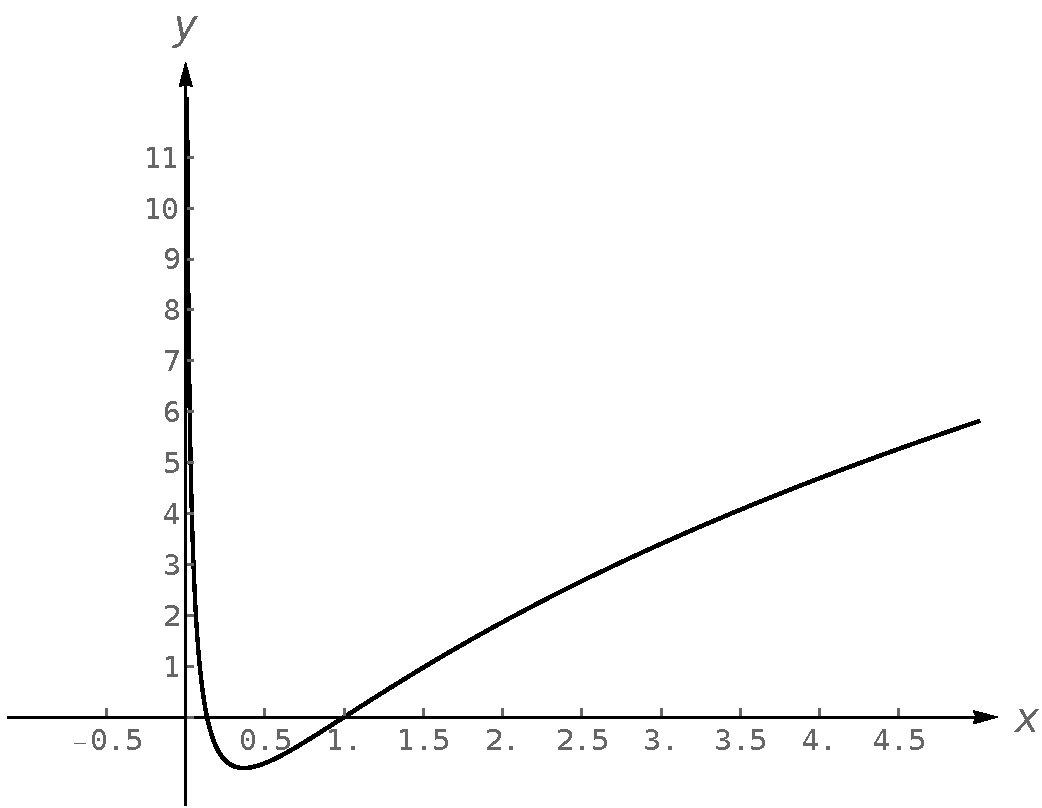
\includegraphics[scale=0.5]{fig_synthese_0}
    }
    \caption{Figure from Exercise~\ref{synthese_0}.}
    \end{figure}
    
\end{Answer}



\begin{Exercise} Determine the angle $\alpha$ between the curve with polar equation $r=e^\theta$, $0\leq\theta\leq\pi$, and the $y$-axis. 
\end{Exercise}

\begin{Answer}
$\alpha = \dfrac{\pi}{4}$    
\end{Answer}


\begin{Exercise} Calculate
$$
\displaystyle\int x\,\cos\left(x^3\right)\,dx
$$
using the MacLaurin series expansion of function $f(x)=\cos(x)$. 
\end{Exercise}

\begin{Answer}
 $
\displaystyle\int x\,\cos\left(x^3\right)\,dx = \sum_{n=0}^{+\infty} \dfrac{(-1)^n\, x^{6n+2}}{(2n)!\, (6n+2)} + C
$   
\end{Answer}



\begin{Exercise}[label=synthese_1] Sketch some level curves of the function $f(x,y)=x^3-y$.
\end{Exercise}

\begin{Answer}
See the figure below. 
\begin{figure}[H]
    \centerline{
   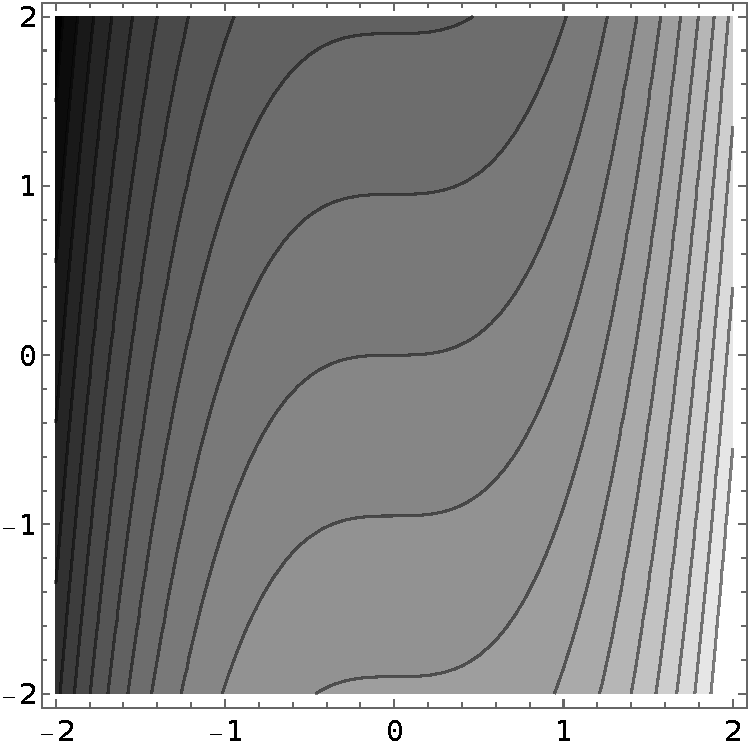
\includegraphics[scale=0.5]{fig_synthese_1}
    }
    \caption{Figure from Exercise~\ref{synthese_1}.}
    \end{figure}
\end{Answer}


\begin{Exercise}[label=synthese_2] Consider 
$$
\int\int_R\Bigl(\left(x^2+y^2\right)^{-3/2}+3\Bigr)\,dA\,,
$$
with 
$$
R=\left\{(x,y)\mid x^2+y^2\leq1\wedge |x|+|y|\geq1\right\}\,.
$$
\Question Sketch the area $R$. 
    \Question Determine appropriate integration boundaries.
    \Question Calculate the integral.
\end{Exercise}

\begin{Answer}

\Question See the figure below. 
\begin{figure}[H]
    \centerline{
   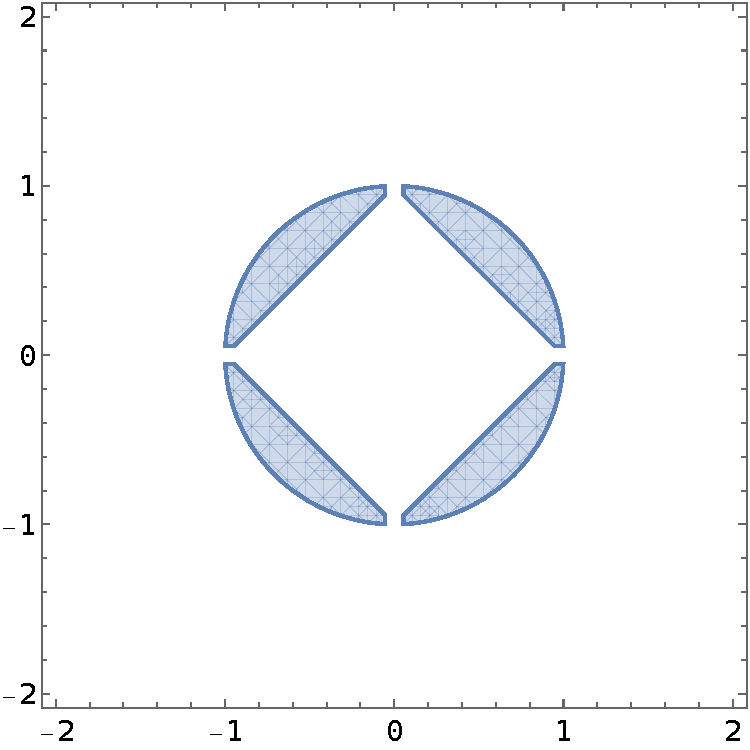
\includegraphics[scale=0.5]{fig_synthese_2}
    }
    \caption{Figure form exercise~\ref{synthese_2}.}
    \end{figure}
\Question $\displaystyle I = 4\int_0^{\pi/2} \int_{1/(\cos(\theta)+r\theta)}^1 \left(r^{-2} +3r\right) dr d\theta$
\Question $I=2+\pi$
    
\end{Answer}




%%%%%%%%%%%%%%%%%%%%%%%%%%%
%Examen Calculus jan/mrt 2021
%%%%%%%%%%%%%%%%%%%%%%%%%%%
\section{Examination January/March 2021}
\begin{Exercise}[label=synthese_3] To contain the coronavirus, numerous measures were taken in 2020 to reduce the reproductive rate $R$. Researchers demonstrated in 2020 that the evolution of the reproductive number can be described as:
$$
R(t)=R_0-\dfrac{1}{2}\left(1+\tanh\left(\dfrac{t-t^*}{T}\right)\right)\left(R_0-R_t\right)\,,
$$
where $R_0$ represents the reproduction number at the start of the corona epidemic, $R_t$ the reproduction number achieved by taking measures, $t^*$ the time it takes before measures are followed, and $T$ the transition time. 

Sketch the graph of $R(t)$ iff $R_0=4$ and $R_t=2$, given the graph of $f(t)=\tanh(t)=\frac{e^{2t}-1}{e^{2t}+1}$ in Figure~\ref{Tanh}. Show the graphs of all transformations required for this. In each case, indicate the asymptotes and the point of intersection with $x$-axis. 
	 \begin{figure}[H]
		\centering
		%\raisebox{0.5cm}{
		\centerline{
			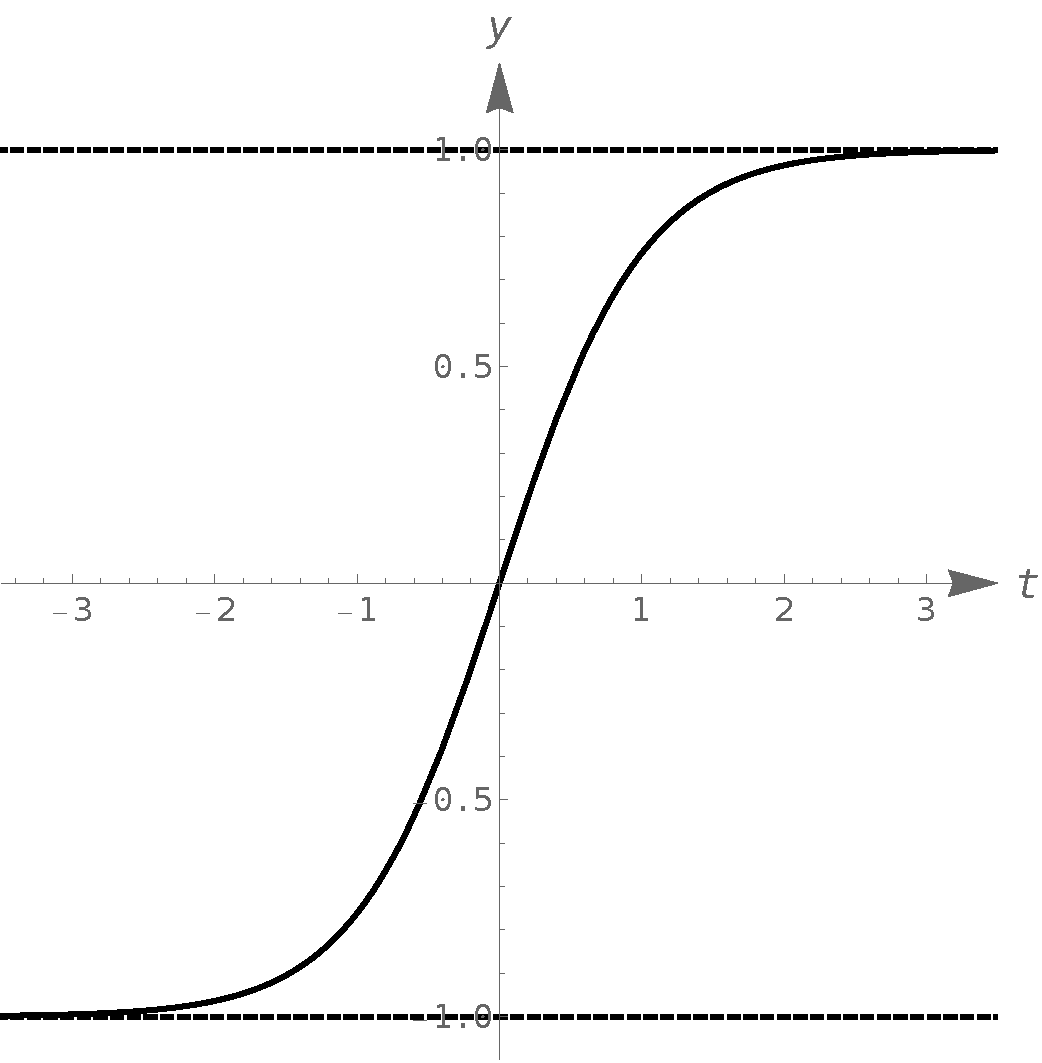
\includegraphics[width=0.4\textwidth]{Tanh.pdf}
		}
		\caption{Graph of the function $f(t)=\tanh(t)$ (full line) and her asymptotes (dotted line).}
		\label{Tanh}
	\end{figure}
\end{Exercise}


\begin{Answer}
See the figure below for $T=5$ and $t^*=5$. 
\begin{figure}[H]
    \centerline{
   \includegraphics[scale=0.5]{fig_synthese_3}
    }
    \caption{Figure from Exercise~\ref{synthese_3}.}
    \end{figure}
\end{Answer}



\begin{Exercise}
Calculate the following limit:
$$
\lim\limits_{x\to+\infty}\ln\left(1+x\right)\,\ln\left(1+\dfrac{1}{x}\right)\,.
$$
\end{Exercise}

\begin{Answer}
  $\lim\limits_{x\to+\infty}\ln\left(1+x\right)\,\ln\left(1+\dfrac{1}{x}\right) = 0$  
\end{Answer}


\begin{Exercise} Consider the function $f(x)=\cos(3\arcsin(x))$ over $[-1,1]$.
\Question Prove that
    $$
    \cos(3\arcsin(x))=\left(1-4x^2\right)\sqrt{1-x^2}\,.
    $$
    \Question Calculate all local and global extremes and indicate for each extremum whether it is a minimum or maximum.
    \Question Calculate the points of infliction.
\end{Exercise}

\begin{Answer}
   
 \Question Prove by saying $y=\arcsin(x)$ and using the trigonometric formulas $\cos(3y) = \cos(y+2y) = \cos(2y)\cos(y) - \sin(2y)\sin(y)$ en $\sin^2(y)+\cos^2(y)=1$.
\Question Global minima: $f\left(\pm\dfrac{\sqrt{3}}{2}\right)=-1$ ; local maxima: $f(\pm 1)=0$ ; global maximum: $f(0)=1$.
\Question Infliction points if $x=\pm\dfrac{\sqrt{3-\sqrt{3}}}{2}$.

\end{Answer}


\begin{Exercise} Calculate
$$
\lim\limits_{x\to0}\dfrac{\left(e^{2x}-1\right)\ln\left(1+x^3\right)}{\left(1-\cos(3x)\right)^2}
$$
using the following Maclaurin series developments (and not l'H\^{o}pital's rule):
$$
e^x=\sum\limits_{n=0}^{+\infty}\dfrac{x^n}{n!}\,,\qquad \sin(x)=\sum\limits_{n=0}^{+\infty}(-1)^n\dfrac{x^{2n+1}}{(2n+1)!}\,,\qquad\text{en }
\ln(x)=\sum\limits_{n=1}^{+\infty}(-1)^{n+1}\dfrac{(x-1)^{n}}{n}\,.$$
\end{Exercise}

\begin{Answer}
$\lim\limits_{x\to0}\dfrac{\left(e^{2x}-1\right)\ln\left(1+x^3\right)}{\left(1-\cos(3x)\right)^2} = \dfrac{8}{81}$    
\end{Answer}


\begin{Exercise} Calculate the integrals below:
\Question $$
\int\dfrac{dx}{x^2\sqrt{x^2+16}}\,
$$
\Question $$
\int\dfrac{dx}{e^{2x}-4e^x+4}\,
$$
\end{Exercise}

\begin{Answer}

\Question $\ds\int\dfrac{dx}{x^2\sqrt{x^2+16}} = -\dfrac{1}{16}\dfrac{\sqrt{16+x^2}}{x} + C$
\Question $\ds\int\dfrac{dx}{e^{2x}-4e^x+4} = \dfrac{\ln(e^x)}{4} - \dfrac{\ln|e^x-2|}{4} - \dfrac{1}{2(e^x-2)} + C$
    
\end{Answer}


\begin{Exercise} On Figure~\ref{Lemniscaat} you can see the lemniscate of Bernouilli, given by the parametric equations
\[ x(\theta) = 3 \sin (\theta), \quad y(\theta) = 2 \sin (2\theta), \quad \text{met } 0 \leq \theta \leq 2\pi. \]

	 \begin{figure}[H]
		\centering
		%\raisebox{0.5cm}{
		\centerline{
			\includegraphics[width=0.4\textwidth]{Lemniscaat.pdf}
		}
		\caption{Graph of the lemniscate of Bernouilli.}
		\label{Lemniscaat}
	\end{figure}

\Question Show that the cartesian equation of the curve is equal to
	\[81 y^2 = 16 x^2(9-x^2) . \]
	\Question Determine the volume of the body that you obtain by rotating the curve about the $x$-axis. 
	\Question Determine the integral that allows you to calculate the volume of the body you obtain by rotating the curve around the $y$-axis.


\end{Exercise}

\begin{Answer}

\Question Prove yourself.
\Question $\ds V=2\pi\int_0^3 y^2\ dx = \dfrac{64\pi}{5}$
\Question $\ds V=36\pi\int_0^{\pi/2} \sin^2(2\theta)\ d\theta$
    
\end{Answer}


\begin{Exercise}
Consider the vector-valued function $\vec{r}(t) = \left(4 \cos(t), 4 \sin(t), 3t \right)$.
\Question Determine the unit tangent vector and unit normal vector for $t=\pi$. 
	\Question Determine an equation of the tangent plane to the curve for $t=\pi$. 
	\Question Parameterize the curve with the arc length parameter.  
	\Question Calculate the curvature in $t=\frac{4 \pi}{3}$.
\end{Exercise}	
\begin{Answer}

\Question $\vec{T}(\pi) = \left(0,-\dfrac{4}{5},\dfrac{3}{5}\right)$\qquad en\qquad $\vec{N}(\pi) = (1,0,0)$
\Question $x=-4$
\Question $\vec{r}(s) = \left(4\cos\left(\dfrac{s}{5}\right),4\sin\left(\dfrac{s}{5}\right),\dfrac{3s}{5}\right)$
\Question $\dfrac{4}{25}$
    
\end{Answer}



\begin{Exercise} The temperature in a room can be described in three dimensions using the following function: 
$$T=f(x,y,z)=10\dfrac{\cos^2\left(xy+z\right)}{\sin\left(\dfrac{y}{x}\right)}\,.$$
\Question Determine the domain and image of $f$.
\Question Determine the directional derivative in the point $P(1,\pi/2,\pi/4)$ in the direction of the vector $\vec{v}=(-1,-1,-1)$. 
\Question Determine the direction in which we must move from the point $P$ to continue to experience maximum cooling. 
\Question Determine the tangent plane to the graph of $f$ at the point $P$.
\Question Determine $f_s$ and $f_t$ if $x=g(s,t)$, $y=h(s,t,v)$ and $z=i(s)$. You should not calculate the occurring partial derivatives explicitly. \end{Exercise}

\begin{Answer}

\Question domain $f = \left\{(x,y,z)\in\mathbb{R}^3\,\left|\, x\neq 0\;\wedge\; \sin\left(\frac{y}{x}\right)\neq 0\right.\right\}$
\Question[] Image $f = [-10,10]$
\Question $D_{\vec{v}} f\left(1,\dfrac{\pi}{2},\dfrac{\pi}{4}\right) = -\dfrac{5\pi+20}{\sqrt{3}}$
\Question $-\vec{\nabla} f\left(1,\dfrac{\pi}{2},\dfrac{\pi}{4}\right) = -(5\pi,10,10) $
\Question $\pi(x-1) +2\left(y-\dfrac{\pi}{2}\right) +2\left(z-\dfrac{\pi}{4}\right)=0$
\Question $f_s = \dfrac{\partial f}{\partial s} = \dfrac{\partial f}{\partial x}\dfrac{\partial x}{\partial s} + \dfrac{\partial f}{\partial y}\dfrac{\partial y}{\partial s} +\dfrac{\partial f}{\partial z}\dfrac{dz}{ds}$
\Question $f_t = \dfrac{\partial f}{\partial t} = \dfrac{\partial f}{\partial x}\dfrac{\partial x}{\partial t} + \dfrac{\partial f}{\partial y}\dfrac{\partial y}{\partial t} $
    
\end{Answer}



\begin{Exercise} Determine the surface of the part of $x^2+y^2+z^2=4z$ that is located inside $z=x^2+y^2$.
\end{Exercise}

\begin{Answer}
$SA = 4\pi$    
\end{Answer}





%%%%%%%%%%%%%%%%%%%%%%%%%%%
%Examen Calculus aug 2021
%%%%%%%%%%%%%%%%%%%%%%%%%%%
\section{Exam August 2021}
\begin{Exercise} Consider the function
$$
f(x)=\alpha x+\beta+\ln\left(e^{-2x}-4\right)\,,
$$
with $\alpha,\,\beta\in\mathbb{R}_0$.
\Question Determine the domain of the function $f$.
    \Question Determine $\alpha$ and $\beta$ such that the line $y=2x-1$ is a skewed asymptote for $f$.
    \Question For $\alpha=4$ and $\beta=-1$
    \begin{enumerate}
    \item[(i)] Determine all asymptotes.
    \item[(ii)] Determine all (local and global) extremes and discuss where $f$ inclines/declines.
    \item[(iii)] Examine the concavity of $f$.
    \end{enumerate}
\end{Exercise}


\begin{Answer}
\Question domain $f = ]-\infty,-\ln(2)[$
\Question $\alpha=4$ and $\beta=-1$
\Question \begin{enumerate}
    \item[(i)] SA: $y=2x-1$\qquad en\qquad VA: $x=-\ln(2)$
    \item[(ii)] There is a maximum if $x=\ln(8^{-1/2})$. The function $f$ inclines over $]-\infty , \ln(8^{-1/2})[$ and declines over $]\ln(8^{-1/2}) , -\ln(2)[$.
    \item[(iii)] The function $f$ is concave over $]-\infty , -\ln(2)[$.
    \end{enumerate}
  
\end{Answer}




\begin{Exercise} Determine the integral below by using a Maclaurin series development for the function in the integrandum. 
\[ \displaystyle \int \ln\left(1+x^2\right) \ dx \] 
\end{Exercise}

\begin{Answer}
$\displaystyle \int \ln\left(1+x^2\right) \ dx = \sum_{n=1}^{+\infty} \dfrac{(-1)^{n+1}\, x^{2n+1} }{n(2n+1)} + C$    
\end{Answer}



\begin{Exercise} Determine
$$
\displaystyle\int\tan(x)\ln\left(\cos(x)\right)\,dx\,.
$$
\end{Exercise}

\begin{Answer}
 $\displaystyle\int\tan(x)\ln\left(\cos(x)\right)\,dx = -\dfrac{1}{2}\ln^2(\cos(x)) + C$   
\end{Answer}





\begin{Exercise} Determine the arc length of the curve described by $$\vec{r}(t)=\left(\cos(t),\sin(t),\ln(\cos(t))\right)$$ voor $t\in[0,\pi/4]$.
\end{Exercise}

\begin{Answer}
$s = \dfrac{1}{2}\ln\left(\left|\dfrac{2+\sqrt{2}}{2-\sqrt{2}}\right|\right)$    
\end{Answer}




\begin{Exercise} We consider a balloon moving in the direction of the maximum wind force. We know from meteorology that the wind always blows from a high-pressure area to a low-pressure area, consequently the wind force is always directed in the direction of maximum air pressure decrease. Now suppose the air pressure is given by following function:
$$
P(x,y)=x^2+\dfrac{y^2}{2}
$$
and let us assume for simplicity that it does not change through time and is independent of height. 
\Question Determine the direction in which the balloon will move from the point $(4,1)$.
    \Question Along which curve through the point $(4,1)$ is the balloon going to move?
    \Question At what point will the balloon end up after waiting a sufficiently long time (no calculation required)? 
\end{Exercise}

\begin{Answer}

\Question $-\vec{\nabla} p(4,1) = (-8,-1)$
\Question $y = \dfrac{\sqrt{x}}{2}$
\Question The origin.
    
\end{Answer}



\begin{Exercise} Consider the double integral
$$
\int\int_Rf(x,y)\,dA\,,
$$
where $A$ is the area in the first quadrant enclosed between\\ $y=2/x$, $y=6/x$, $y=x-1$ and $y=x+1$. Determine the boundaries of this double integral if
\Question $dA=dx\,dy$
\Question $dA=dy\,dx$
\end{Exercise}

\begin{Answer}

\Question $\displaystyle\int_1^2\int_{2/y}^{y+1} f(x,y)\, dxdy + \int_2^3\int_{y-1}^{6/y} f(x,y)\, dxdy$
\Question $\displaystyle\int_1^2\int_{2/x}^{x+1} f(x,y)\, dydx + \int_2^3\int_{x-1}^{6/x} f(x,y)\, dydx$
    
\end{Answer}



\begin{Exercise} Consider the vector field
$$
\vec{F}=\left(2xe^{-y},2y-x^2e^{-y}\right)
$$
\Question Show that this vector field is conservative. 
\Question Calculate the line integral along the polar curve $r(\theta)=\theta$ between $\theta=0$ and $\theta=\pi/2$. 
\end{Exercise}

\begin{Answer}

\Question Prove for yourself that $\text{rot}\,\vec{F} = 0$.
\Question $\displaystyle\int_C \vec{F}\cdot d\vec{r} = \dfrac{\pi^2}{4}$
    
\end{Answer}



\fi

\section{Oplossingen}